\documentclass[envcountsect,usenames,dvipsnames]{beamer}

%normal
\usepackage{beamerthemebars}
\usepackage{lmodern}
\usepackage{multicol}
\usepackage{subfigure}
\usepackage{graphicx} % Allows including images
\usepackage{booktabs}
\usepackage{bbm}
\usepackage{bm}
\usepackage{amsmath}
\usepackage{mathtools}
\usepackage{booktabs}
\usepackage{tikz}
\usepackage{nicefrac}
%\usepackage[round]{natbib} 
%\usepackage{enumitem}
\usepackage[export]{adjustbox}



\usepackage[style=authoryear,backend=bibtex]{biblatex}
\bibliography{bib} 

\DeclareMathOperator{\AV}{AVar}

\usetikzlibrary{arrows,matrix,positioning,fit}% For nice arrow tips
\newcommand{\tikzcircle}[2][red,fill=red]{\tikz[baseline=-0.5ex]\draw[#1,radius=#2] (0,0) circle ;}


\tikzset{
    !/.style = {
        fill=red!20,
    },
    mymatrix/.style = {
        matrix of math nodes,
        left delimiter  = [,
        right delimiter = ],
        nodes={minimum width=4ex},
    }
}

\tikzset{ 
    !/.style = {
        fill=red!20,
    },
    mymatrix2/.style = {
        matrix of math nodes,
        left delimiter  = (,
        right delimiter = ),
        nodes={minimum width=1ex},
    }
}

 \usepackage[boxed,linesnumberedhidden]{algorithm2e} % pour l'algo
\SetAlCapSkip{0.4cm}

\usetikzlibrary{positioning}
\usetikzlibrary{arrows}

\usetheme{AnnArbor}
\usecolortheme{wolverine} 


\newcommand\mytikzmark[3][]{%
  \tikz[remember picture,baseline=(#2.base)]{\node(#2)[outer sep=0pt,#1]{#3};}%
}
\tikzset{block/.style={minimum width=1.1 em, minimum height= 1em, rounded corners= 4pt}}


\DeclareMathOperator*{\argmax}{argmax}
\DeclareMathOperator*{\diag}{diag}
\DeclareMathOperator*{\plim}{plim}
\DeclareMathOperator*{\argmin}{argmin}
\DeclareMathOperator*{\argzero}{argzero}
\DeclareMathOperator*{\cov}{cov}
\DeclareMathOperator*{\corr}{corr}
\DeclareMathOperator*{\mean}{mean}
\DeclareMathOperator*{\modulo}{mod}
\DeclareMathOperator*{\var}{var}
\DeclareMathOperator*{\tr}{tr}
\DeclareMathOperator*{\WVIC}{WVIC}
\DeclareMathOperator*{\model}{\mathcal{M}}


\let\C\undefined
\DeclareMathOperator{\C}{\textup{C}}

\DeclareSymbolFont{lettersA}{U}{txmia}{m}{it}
\DeclareMathSymbol{\real}{\mathord}{lettersA}{"92} 
\DeclareMathSymbol{\field}{\mathord}{lettersA}{"83}

%redefined colors for beamer
\definecolor{beamer@UIUCblue}{RGB}{9,49,98}
\definecolor{beamer@UIUCorange}{RGB}{240,240,240}
% taken from 
% http://identitystandards.illinois.edu/graphicstandardsmanual/generalguidelines/colors.html

\definecolor{beamer@UIUCgray}{RGB}{210,210,210}
\definecolor{beamer@UIUCgray2}{RGB}{244,244,244}
\definecolor{beamer@myorange}{RGB}{244,127,36}

\setbeamercolor{frametitle}{fg=beamer@UIUCblue,bg=beamer@UIUCgray}
\setbeamercolor{normal text}{fg=black}
\setbeamercolor{title}{fg=beamer@UIUCblue,bg=beamer@UIUCorange}
\setbeamercolor{item projected}{fg=white,bg=beamer@UIUCblue}
%boxes
\setbeamercolor{block title}{fg=beamer@UIUCblue,bg=beamer@UIUCorange}
\setbeamercolor{block body}{fg=blue,bg=beamer@UIUCblue!80}
\setbeamercolor{title in head/foot}{fg=beamer@UIUCblue,bg=beamer@UIUCgray}
\setbeamercolor{author in head/foot}{fg=white,bg=beamer@UIUCblue}
\setbeamercolor{institute in head/foot}{fg=white,bg=beamer@UIUCorange}
\setbeamercolor{date in head/foot}{fg=beamer@UIUCblue,bg=beamer@UIUCorange}
\setbeamercolor{section in head/foot}{fg=white,bg=beamer@UIUCblue}
\setbeamercolor{subsection in head/foot}{fg=beamer@UIUCblue,bg=beamer@UIUCorange}

\definecolor{light-gray}{gray}{0.7}
\newcommand{\light}[1]{\textcolor{light-gray}{#1}}

\setbeamercolor{button}{bg=beamer@UIUCgray,fg=beamer@UIUCblue}

\def\X{\mathbf X}
\def\y{\bm y}
\def\bbeta{\bm \beta}
\def\bvarep{\bm \varepsilon}
\def\btheta{\bm \theta}
\def\bTheta{\bm \Theta}
\def\bgamma{\bm \gamma}
\def\g{\mathbf{g}}
\def\W{\mathbf{W}}
\def\A{\mathbf{A}}
\def\simiid{\stackrel{iid}{\sim}}

\DeclareMathOperator{\hatBtheta}{\hat{\bm{\theta}}}
\DeclareMathOperator{\Btheta}{\bm{\theta}}
\let\emptyset\varnothing

%override title link color 
\makeatletter
\renewcommand\insertshorttitle[1][]{%
  \beamer@setupshort{#1}%
  \let\thanks=\@gobble% 
  \ifnum\c@page=1%
  \hyperlinkpresentationend{\beamer@insertshort{\usebeamercolor*[fg]{title in head/foot}\beamer@shorttitle}}%
  \else%
  \hyperlinkpresentationstart{\beamer@insertshort{\usebeamercolor*[fg]{title in head/foot}\beamer@shorttitle}}%
  \fi}
\makeatother

\usepackage{etoolbox}
\makeatletter
\patchcmd{\beamer@section}
  {\def\insertsectionhead{\hyperlink{Navigation\the\c@page}{#1}}}
  {\def\insertsectionhead{\hyperlink{Navigation\the\c@page}{\usebeamercolor*[fg]{section in head/foot}#1}}}
  {}{}
\patchcmd{\beamer@subsection}
  {\def\insertsubsectionhead{\hyperlink{Navigation\the\c@page}{#1}}}
  {\def\insertsubsectionhead{\hyperlink{Navigation\the\c@page}{\usebeamercolor*[fg]{subsection in head/foot}#1}}}
  {}{}
\makeatother

%\setbeamercolor{palette tertiary}{bg=beamer@UIUCblue,fg=white}
%\setbeamercolor{palette secondary}{bg=beamer@UIUCgray,fg=white}
%\setbeamercolor{palette primary}{bg=beamer@UIUCorange,fg=white}

\usepackage{marvosym}

\beamertemplatenavigationsymbolsempty %hides navigation.
\usepackage{graphicx}
\usepackage{comment}
\usepackage{hyperref}
\usepackage{amssymb,amsmath}
\usepackage{multirow}
\usepackage{upgreek}

\makeatletter
\def\th@mystyle{%
    \normalfont % body font
    \def\inserttheoremblockenv{exampleblock}
  }
\makeatother
\theoremstyle{mystyle}
\newtheorem{Remark}{Remark}
\newtheorem{Property}{Property}
%\renewcommand{\theRemark}{\Alph{Remark}}
\DeclarePairedDelimiter\floor{\lfloor}{\rfloor}

\setbeamertemplate{theorems}[ams style] 
\renewcommand*{\bibfont}{\scriptsize}

\usenavigationsymbolstemplate{}

%flow charts
\usepackage{tikz}
\usetikzlibrary{shapes,arrows} 
\tikzset{every picture/.style={line width=0.75pt}} %set default line width to 0.75pt        
 
 
\author[St\'ephane Guerrier]{St\'ephane Guerrier}
\institute[]{
%Department of Statistics \& Institute for CyberScience\\
Pennsylvania State University\\
Department of Statistics \& Institute for CyberScience \vspace{0.25cm}\\ This document was prepared with the help of \\Dr. Roberto Molinari (Penn State), Dr. Mucyo Karemera (Penn State), \\Gaetan Bakalli (U. Geneva), Haotian Xu (U. Geneva) \& Yuming Zhang (Penn State)\vspace{0.1cm}%\\
%Material available online: \href{smac-group.com}{smac-group.com}

%\vspace{0.5cm} joint work with \\ 
%\vspace{0.3cm} Roberto Molinari (UCSB), Jan Skaloud (EPFL),\\ Yannick Stebler (u-blox) \& Maria-Pia Victoria-Feser 
%(UniGe)}

\begin{center}
	\includegraphics[width=0.25\textwidth]{Images/licence.png}
\end{center}
\vspace{-0.3cm}
}


 
\begin{document} 
\defbibheading{Ref}{\frametitle{References}}


\date[April 2018]{\footnotesize Last update: April 2018}

\title[Inertial Sensor Stochastic Calibration]{
%\begin{columns}
%\column{.15\textwidth} 
%\hspace{.2in}
%\vspace{.1in} 
%\phantom{fs}\vspace{-.25in} 
%\begin{center}
%\includegraphics[width = 0.7in]{logo.png}  	
%\end{center}
%\column{.15\textwidth} 
%\column{.85\textwidth}
\begin{center}
	{An Introduction to Inertial Sensor Stochastic Calibration}
\end{center}
%\end{columns}
}
\frame{\titlepage}

%\begin{frame}
%\frametitle{Overview} % Table of contents slide, comment this block out to remove it
%\tableofcontents % Throughout your presentation, if you choose to use \section{} and \subsection{} commands, these will automatically be printed on this slide as an overview of your presentation
%\end{frame}

\setbeamercolor{block title}{fg = white, bg = beamer@UIUCblue}
\setbeamercolor{block body}{fg=black,bg=beamer@UIUCgray2}

\setbeamercolor{block title alerted}{fg = white, bg = beamer@myorange}
\setbeamercolor{block body alerted}{fg=black,bg=beamer@UIUCgray2}

\setbeamercolor{block title example}{fg = beamer@UIUCblue, bg = beamer@UIUCgray}
\setbeamercolor{block body example}{fg=black,bg=beamer@UIUCgray2}


\section{GMWM-based IMU Calibration}\newrefsection


\subsection{Introduction}
%\begin{frame}{Collaborative Research Project}
%    \begin{figure}
%		   \centering
%		  \includegraphics[width = 12cm]{Images/poeple_map.pdf}
%		\end{figure}
%\end{frame}


\begin{frame}{Outline}
\small
\begin{multicols}{2}
  \tableofcontents
\end{multicols}
\end{frame}

\begin{frame}{Outline}
\small
\begin{multicols}{2}
  \tableofcontents[currentsection]
\end{multicols}
\end{frame}

\begin{frame}{Introduction}
\begin{block}{{General Framework:}}
	\begin{itemize}
		\item A \textbf{{\color{beamer@UIUCblue} new framework for inertial sensor calibration.}}
		\item It is based on the \textbf{{\color{beamer@UIUCblue}Generalized Method of Wavelet Moments (GMWM)}} of \cite{guerrier2013wavelet}, which is a new statistical approach to estimate the parameters of (complex) time series models.
		\item The GMWM is able to estimate efficiently time series models which are commonly used to describe the errors of inertial sensors.
		\item This calibration approach provides considerable improvements (in terms of navigation performance) compared to existing methods.
		\item This methodology is \textbf{{\color{beamer@UIUCblue}robust}} (potentially applicable for FDI purposes) and is able to \textbf{{\color{beamer@UIUCblue}automatically select a suitable model}} (or rank models).
	\end{itemize}
\end{block}
\end{frame}

\begin{frame}{Inertial Sensors} 
	\begin{exampleblock}{Inertial Measurement Unit (IMU):}
		An IMU is composed of accelerometers and gyroscopes. Very widely employed as part of ``integrated'' navigation systems, a few examples:
		\begin{itemize}
			\item Robots
			\item (Small) \textbf{{\color{beamer@UIUCblue}Unmanned Aerial Vehicles}} (e.g. 3D modeling, search and rescue, etc)
			\item Autonomous underwater vehicles (e.g. water quality monitoring)
			\item Sport (e.g. ski, swimming, etc)
			\item Virtual reality (e.g. video games, movies, etc) %\includegraphics[width = 1cm]{Images/ted}
		\end{itemize} 
	\end{exampleblock}
\end{frame}

\begin{frame}{IMU in Navigation}
	\begin{exampleblock}{ }
		\begin{itemize}
			\item \textbf{{\color{beamer@UIUCblue}GPS clearly dominates}} the current position and navigation market.
			\item It provides the whole range of navigation at very low cost.
			\item It is also highly portable, has low power consumption and is well suited for integration with other sensors.
			\item Unfortunately, \textbf{{\color{beamer@UIUCblue}GPS does not work in all environments.}}
			\item An IMU presents characteristics that are very different from GPS.
			\item It provides a \textbf{{\color{beamer@UIUCblue}navigation solution when GPS-signals are unavailable}}.
			\item It has higher sampling rate and \textbf{{\color{beamer@UIUCblue}greatly improves orientation estimation}}.
			\item The main challenge with IMUs (MEMS in particular) are their large sensor errors, which rapidly degrade the navigation
			performance.
		\end{itemize}
	\end{exampleblock}
\end{frame}

\begin{frame}{Inertial Navigation}	 
\begin{figure}
	\centering
	\includegraphics[width = 12cm]{Images/INS}
\end{figure}
\vspace{-0.3cm}

\scriptsize{\textbf{{\color{beamer@UIUCblue}Source:}} \cite{stebler2012PHD}}
\end{frame}

\begin{frame}{IMU + other sensors (GPS)}	 
\begin{figure}
	\centering
	\includegraphics[width = 12cm]{Images/Int_INS}
\end{figure}
\vspace{0.15cm}
\scriptsize{\textbf{{\color{beamer@UIUCblue}Source:}} \cite{stebler2012PHD}}
\end{frame}

\begin{frame}{Helicopter-based mobile mapping}

	\vspace{-0.35cm}

	\begin{center}
		\footnotesize{\textit{Ecole Polytechnique F\'{e}d\'{e}rale de Lausanne (EPFL)}}
	\end{center}

	\vspace{-0.6cm}

	  	\begin{columns}
		\begin{column}{0.65\textwidth}
			\vspace{0.1cm}
			\begin{figure}
			    \centering
			  \includegraphics[width = 4.5cm]{Images/scan2MapLogo}
			\end{figure}
			\vspace{-0.5cm}
			\begin{figure}
			    \centering
			  \includegraphics[width = 7cm]{Images/Scan2Map}
			\end{figure}
		\end{column}
		\begin{column}{0.35\textwidth}
			\begin{figure}
			    \centering
			  \includegraphics[width = 3.4cm]{Images/Scan2MapExample}
			\end{figure}
		\end{column}
		\end{columns}
\end{frame}


\begin{frame}{UAV for search and rescue operations}
	
	\vspace{-0.7cm}
	
	\begin{center}
		\footnotesize{\textit{Institut de Geom\`{a}tica (Barcelona), EPFL, ...}}
	\end{center}
	
	\vspace{-0.2cm}
	 
	\begin{columns}
	\begin{column}{0.45\textwidth}
		\vspace{-0.5cm}
		\begin{figure}
		    \centering
		  \includegraphics[width = 4.8cm]{Images/SearchNrescue}
		\end{figure}
	\end{column}
	\begin{column}{0.55\textwidth}
		
	\begin{figure}
		\centering
		\includegraphics[width = 6cm]{Images/thermo1}
	\end{figure}
	\vspace{-0.6cm}
	\begin{figure}
	 	\centering
		\includegraphics[width = 6cm]{Images/thermo2}
	\end{figure}
	\end{column}
	\end{columns}
\end{frame}


\begin{frame}{IMU Calibration}
	\begin{block}{Errors in Inertial Sensors}
		\begin{itemize}
			\item Possible causes:
			\begin{itemize}
				\item Non-orthogonalities of the sensor axes
				\item Environmental conditions (e.g. temperature)
				\item Electronics
				\item Dynamics
				\item ...
			\end{itemize}
			\item Error types:
			\begin{itemize}
				\item Deterministic (calibration models, physical models, ... )
				\item \textbf{{\color{beamer@UIUCblue}Random error components}} (typically latent time series models,...)
			\end{itemize}
		\end{itemize}
	\end{block}
	
	\begin{block}{Correct stochastic sensor error modeling implies:}
	\begin{itemize}
		\item  Correct stochastic assumptions for inference
		 \item \textbf{{\color{beamer@UIUCblue}Better navigation or post-processing performance}}
	\end{itemize}
\end{block}
\end{frame}


\begin{frame}{Effect on position of error model}
	\begin{exampleblock}{Emulation setting:}
		\begin{itemize}
			\item Suppose the following model for inertial sensors (WN + GM):
			%
			\small
			\begin{equation*}
				\begin{aligned}
					{Y_t} &= {\exp(-\beta \Delta t ) Y_{t-1} + \varepsilon_t,} \;\; { \varepsilon_t \stackrel{iid}{\sim} \mathcal{N}(0,\sigma_{GM}^2 (1 - \exp(-2 \beta \Delta t)))}\\
					{ X_t} & {\stackrel{iid}{\sim} \mathcal{N}(0,\sigma^2),} \;\; 
					{Z_t = X_t + Y_t.}
				\end{aligned}
			\end{equation*}
			\normalsize
			%
			\item Consider the following three models:
			
			\begin{table}
			    \centering
			    \small{
			    \setlength{\tabcolsep}{8pt}
			    \begin{tabular*}{0.8\textwidth }{l l c c c }
			    \toprule
			    \textbf{Sensor}     & \textbf{Scenario}     & $\beta$  & $\sigma_{GM}$     & $\sigma_{WN}$  \\
			    \midrule
			    Acc. & {\color{beamer@myorange}Correct model} & $10^{-4}$ & $50.0$ & $70.0$     \\
			    & {\color{beamer@UIUCblue}Wrong $\beta$} & $10^{-2}$ & $50.0$ & $70.0$     \\
			    & {\color{beamer@UIUCblue}Without GM} & -- & -- & $70.0$     \\[1mm]
			    \hdashline\\[-3mm]
			    Gyro. & {\color{beamer@myorange}Correct model} & $10^{-4}$ & $10.0$ & $30.0$ \\
			    & {\color{beamer@UIUCblue}Wrong $\beta$} & $10^{-2}$ & $10.0$ & $30.0$ \\
			    & {\color{beamer@UIUCblue}Without GM} & -- & -- & $30.0$ \\
			    \bottomrule
			    \end{tabular*}
			}
			\end{table}
			\vspace{-0.2cm}
		\end{itemize}
	\end{exampleblock}  
	
\end{frame}

\begin{frame}{Effect on position of error model}
	\begin{figure}
	  \centering
	 	%\includegraphics[width=0.6\textwidth]{images/ch5/planimetry}
	 \subfloat{\label{fig:plani}\includegraphics[height=0.45\textwidth]{Images/planimetry}}
	  \subfloat{\label{fig:alti}\includegraphics[height=0.45\textwidth]{Images/altimetry}}
	  \label{fig:traj}
	\end{figure}
\end{frame}

%\begin{frame}{GMWM to calibrate IMUs} 
%	\begin{block}{IMU are subject to measurement errors...}
%		\begin{enumerate}
%			\item IMUs are corrupted by \textbf{{\color{beamer@UIUCblue}stochastic errors}} (typically modeled as latent time series).
%			\item These errors are modeled using stochastic processes in a ``navigation filter''.
%			\item The ``quality'' of the estimated error model has a \emph{great impact on the ``navigation'' performance} (e.g. orientation, position, ...).
%			\item There exist (at least) three methods to estimate IMU errors, {the GMWM is one of them}.
%			\item \textbf{{\color{beamer@UIUCblue}GMWM was designed for such problems and performs very well.}}
%		\end{enumerate}
%	\end{block}
%\end{frame}


\begin{frame}{An easy latent time series model}
	 	\begin{columns}
		\begin{column}{0.6\textwidth}
			\vspace{0.3cm}
			\begin{figure}
				\vspace{-0.8cm}
			    \centering
			  \includegraphics[width = 7cm]{Images/DR_WN_Pub}
			\end{figure}
		
		\end{column}
		\begin{column}{0.35\textwidth}
		\begin{block}{Remarks:}
			\begin{itemize}
			\item Simple linear regression model:
			%
			\begin{equation*}
				\begin{aligned}
						y_t &= \omega t + \varepsilon_t\\
						 \varepsilon_t &\stackrel{iid}{\sim} \mathcal{N}\left(0, \sigma^2\right)
				\end{aligned}
			\end{equation*}
			
			\item MLE is perfectly fine.
			
			\item \textbf{{\color{beamer@UIUCblue}What if we add an AR1 process?}}
			\end{itemize}
		\end{block}
		\end{column}
		\end{columns}
\end{frame}

\begin{frame}{Adding an autoregressive process}
 	\begin{columns}
	\begin{column}{0.6\textwidth}
		\vspace{0.3cm}
		\begin{figure}
			\vspace{-0.8cm}
		    \centering
		  \includegraphics[width = 7cm]{Images/DR_WN_ARPub}
		\end{figure}
	
	\end{column}
	\begin{column}{0.35\textwidth}
	\begin{block}{Remarks:}
		\begin{itemize}
			\item Not a linear regression model but a \textbf{{\color{beamer@UIUCblue}state space model}}.
			\item Computing the likelihood is not an easy task (Kalman filter).
			\item \textbf{{\color{beamer@UIUCblue}MLE (in fact EM-KF) fails}}.
		\end{itemize}
	\end{block}
	\end{column}
	\end{columns}	
\end{frame}

\begin{frame}{Estimation of Latent Time Series Models}
	\begin{block}{Existing methods:}
		\begin{itemize}
			\item {\color{beamer@UIUCblue}Transforming into a ``non-latent'' model (e.g. ARMA)}
			\begin{itemize}
				\item Does not work in general.
				\item Tends to diverge when one latent time series is ``close'' to unit root.
				\item Difficult to ``inverse''.
			\end{itemize}
			\item {\color{beamer@UIUCblue}MLE of an associated state-space (possibly using EM algorithm)}
			\begin{itemize}
				\item Computationally intensive.
				\item Systematically diverges with ``complex'' models.
				\item A lot of work is needed for a new model (see \cite{stebler2011constrained}).
			\end{itemize}
			\item {\color{beamer@UIUCblue}``Graphical'' method}
			\begin{itemize}
				\item Limited to a few possible models.
				\item Not consistent in general (see \cite{guerrier2016theoretical}).
				\item ``Inefficient'' (see \cite{guerrier2016theoretical}).
			\end{itemize}
		\end{itemize}
	\end{block}
\end{frame}

\begin{frame}{Looking differently at a time series using the Allan variance}
 	\begin{columns}
		\begin{column}{0.6\textwidth}
			
			\vspace{-0.6cm}
				\begin{figure}
	    			\centering
	  				\includegraphics[width = 7cm]{Images/AV}
				\end{figure}
	
			\end{column}
			\begin{column}{0.35\textwidth}
				\begin{block}{Remarks:}
		\begin{itemize}
		\item Proposed by \textit{Allan, Proc. IEEE, 1966}
		
		\item Originally intended to study the stability of atomic clocks.
		
		\item Allan Variance is closely related to the (haar) Wavelet Variance.
		\end{itemize}
	\end{block}
		\end{column}
		\end{columns}
\end{frame}

\begin{frame}{The Wavelet (Allan) variance}
	\vspace{-0.85cm}
	\begin{figure}
	    \centering
	  \includegraphics[width = 8.5cm]{Images/WN}
	\end{figure}
\end{frame}

\begin{frame}{Initial idea:}
	\begin{alertblock}{Match the WV:}
		\begin{itemize}
			\item Exploit the relationship that exists between the model $F_{\bm{\theta}}$ and the WV $\bm{\nu}(\bm{\theta})$ (i.e. \textbf{{\color{beamer@UIUCblue} mapping $\bm{\theta} \mapsto \bm{\nu}(\bm{\theta})$}}).
			\item ``Inverse'' this mapping by minimizing some discrepancy between empirical WV ($\hat{\bm{\nu}}$) and the theoretical WV $\bm{\nu}(\bm{\theta})$.
			\item This should provide an approximation of the point $\bm{\theta}(\hat{\bm{\nu}})$.
		\end{itemize}
	\end{alertblock}
\end{frame}

\subsection{Wavelet Variance}


\begin{frame}{Wavelet Variance}
	\begin{block}{Empirical WV:}
\begin{itemize}
\item The WV ($\nu_j^2$) is the \textbf{{\color{beamer@UIUCblue}variance of wavelet coefficients}} for the scale $j$.
\item Wavelet coefficients ($W_{j,t}$) are weighted averages computed on the series $Y_t$.
\item The weights are called wavelet filters $h_j$: e.g. the Haar wavelet filter.
\item The wavelet filters give non-zero weights to observations at a given lag (window sizes of length $L_j$). Hence, there are as many WV as there are scales.
\item The wavelet filters can be computed on consecutive windows, or on overlapping windows (to get $\widetilde{W}_{j,t}$ using $\tilde{h_j}$). Overlapping windows lead to more efficient estimators (such as the MODWT).
\end{itemize}
%and where $\tilde h_{j,l}$ wavelet filters (based on MODWT).
\end{block}

\end{frame}

	
\begin{frame}{Wavelet Variance}
	\begin{block}{Wavelet Variance}
The Wavelet Variance (WV) is the variance of the wavelet coefficients, i.e.
%
\begin{equation*}
 \nu_j^2 = \text{var} \left ( W_{j,t} \right ), \; \; \text{where} \; \; W_{j,t} = \sum_{l=0}^{L_j-1} h_{j,l} y_{t-l}, \;t \in \mathbb{Z}
 %_{F_{\bm{\theta}}}
\label{eq:WVtheo}
 \end{equation*}
%
and where $h_{j,l}$ are wavelet filters based on MODWT.
\end{block}

\begin{exampleblock}{Remark}
    The Allan Variance (AV) is a {\color{beamer@myorange}\textbf{special case}} of the WV, in fact ${\phi}^2_j = 2 \nu^2_{j}$ where $\nu^2_{j}$ is based on Haar wavelet.  
\end{exampleblock}
\end{frame}


\begin{frame}{Estimation of the WV}
	\begin{block}{MODWT estimator:}
		A consistent estimator for $\nu_j^2$ is given by the MODWT estimator defined in \cite{percival2000wavelet}
		%
		\begin{equation*}
		 \hat{\nu}_j^2 = \frac{1}{M(T_j)} \sum_{t\in T_j} W_{j,t}^2.
		 \label{eq:WaveVar}
		\end{equation*} 
		%
		\end{block}
		\begin{alertblock}{Theorem: Asymptotic Normality}
		    \cite{serroukh2000statistical} show that under suitable conditions
		%
		\begin{eqnarray*}
				\sqrt{M(T_j)}\left(\hat{\nu}_j^2-\nu_j\right) \xmapsto[T\rightarrow\infty]{\mathcal{D}} \mathcal{N}\left(0,S_{W_j}(0)\right).
		\end{eqnarray*}
		%
	\end{alertblock}
\end{frame}


\begin{frame}{A more general theorem}
		\begin{alertblock}{Theorem: Multivariate Extension}
			We extended this result to the multivariate case and demonstrated that under some regularity conditions
			%
			\begin{eqnarray*}
	    	\sqrt{T}\left(\hat{\bm{\nu}}-\bm{\nu}\right) \xmapsto[T\rightarrow\infty]{\mathcal{D}} \mathcal{N}\left(0,\mathbf{\Sigma}\right)
			\end{eqnarray*}
			%
			where
			$\mathbf{\Sigma}=[\sigma^2_{kl}]_{k,l=1,\ldots,J}$.
			\end{alertblock}
			
			\begin{exampleblock}{Remark}
					This theorem generalizes \cite{serroukh2000statistical} result and enables to compute the (asymptotic) covariance between the WV (or the AV) at two different scales.

			  \end{exampleblock}
\end{frame}


\begin{frame}{Theoretical WV}
	\begin{block}{WV implied by $F_{\bm{\theta}}$:}
		\small
		Given a model $F_{\bm{\theta}}$ one can compute the theoretical WV as: 
		%
		\begin{equation*}
				 \nu_{j} = f\left( \bm{\theta} \right) = \int_{-1/2}^{1/2} |{\widetilde H}_j(f)|^2 S_{F_{\bm\theta}}(f) df.
		\end{equation*}
		%
	\end{block} 
	
	\begin{exampleblock}{Example:}
		\small
		Consider an AR1:
		%
		\vspace{-0.1cm}
		\[ 
						Y_t = \phi Y_{t-1} + \varepsilon_t, \;\; \varepsilon_t \overset{iid}{\sim}  \mathcal{N}\left( 0 , \sigma^2 \right), \;\;  t = 1, ... , T
				\]
		\vspace{-0.1cm}
		%
		With $\tau_j = 2^j$, the theoretical (Haar) WV of such process is given by
		%
		\vspace{-0.1cm}
		\[ 
		  \nu_{j} =\frac{\left( \frac{\tau_j}{2} - 3 \phi - \frac{\tau_j \phi^2}{2} + 4\phi^{\frac{\tau_j}{2} + 1} - \phi^{\tau_j + 1} \right) \sigma^2}{\frac{\tau_j^2}{2} \left(1 - \phi \right)^2 \left(1 - \phi^2 \right)}
				\]
		\vspace{-0.1cm}
		% 
	\end{exampleblock}
\end{frame}


\begin{frame}{WV of latent time series models}
	\begin{block}{A very useful property:}
		Suppose we have
		%
		\begin{equation*}
			Y_t = X_t^{(1)} + ... + X_t^{(k)},
		\end{equation*}
		%
		then the PSD of $Y_t$ is
		%
		\begin{equation*}
			S_{Y_t} = S_{X_t^{(1)}} + ... + S_{X_t^{(k)}},
		\end{equation*}
		%
		so the WV of $Y_t$ is given by
		%
		\begin{equation*}
			\nu_{Y_t, j} = \int_{-1/2}^{1/2} |{\widetilde H}_j(f)|^2 \left(\sum_{i = 1}^{k} S_{X_t^{(i)}} \right) df = \sum_{i = 1}^{k} \nu_{X_t^{(i)}, j}.
		\end{equation*}
		%
	\end{block}
\end{frame}

\subsection{GMWM Framework}


\begin{frame}{Principle of the GMWM}

	\begin{figure}
	\vspace{-0.5cm}
	    \centering
	  \includegraphics[width = 8cm]{Images/AR1WVtheo.pdf}
	\end{figure}
\end{frame}


\begin{frame}{Principle of the GMWM}

	\begin{figure}
		\vspace{-0.5cm}

	    \centering
	  \includegraphics[width = 8cm]{Images/AR12WVempir.pdf}
	\end{figure}
\end{frame}

\begin{frame}{The GMWM estimator}
		\begin{block}{Definition:}
			The GMWM estimator is the solution of the following optimization problem
			%
			\begin{equation*}
			\hat{\bm{\theta}} = \underset{\bm{\theta} \in \bm{\Theta} }{\argmin} \;
			\left(\hat{\bm{\nu}} - \bm{\nu}(\bm{\theta})\right)^{T} \bm{\Omega} \left(\hat{\bm{\nu}} - \bm{\nu}(\bm{\theta})\right),
			\label{eq:indirectEstimator}
			\end{equation*}
			%
			in which $\bm{\Omega}$, a positive definite weighting matrix, is chosen in a suitable manner such that the above quadratic form is convex.
			\end{block}
			
		\begin{alertblock}{Theorem: Consistency}	
			$\hat{\bm{\theta}}$ is a consistent estimator of $\bm{\theta}$ (under some regularity conditions) for a large class of (latent or composite) models.
		\end{alertblock}	
\end{frame}


\begin{frame}{Asymptotic distribution of $\hat{\bm{\theta}}$}
		\begin{alertblock}{Theorem: Asymptotic Normality}	
			We showed that (under some regularity conditions)
			%
			\begin{eqnarray*}
				\sqrt{T}\left(\hat{\bm{\theta}}-{\bm{\theta}}_0 \right) \xmapsto[T\rightarrow\infty]{\mathcal{D}} \mathcal{N}\left(0,\mathbf{V}\right),
			\end{eqnarray*}
			%
			where $\mathbf{V} = \mathbf{B} \bm{\Sigma} \mathbf{B}^T$,	$\mathbf{B} = \left(\mathbf{D}^T \bm{\Omega} \mathbf{D} \right)^{-1} \mathbf{D}^T \bm{\Omega}$, $\mathbf{D} =\partial \bm{\nu}(\bm{\theta}) / \partial \bm{\theta}^T$ and $\bm{\Sigma}$ 
			%and $\mathbf{V}_{\hat{\bm{\phi}^{\star}}}$ are 
			is the asymptotic covariance matrix of $\hat{\bm{\nu}}$.
		\end{alertblock}
		
		\begin{exampleblock}{Choosing $\bm{\Omega}$:}	
	The most efficient estimator is (asymptotically) obtained by choosing $\bm{\Omega} = \bm{\Sigma}^{-1}$, leading then to  $\mathbf{V} =  (\mathbf{D}^T \bm{\Sigma}^{-1} \mathbf{D})^{-1}$.
		\end{exampleblock}
\end{frame}

%\begin{frame}{Principle of the GMWM estimator}
%	\begin{figure}
%	    \centering
%	  \includegraphics[width = 9cm]{Images/schema}
%	\end{figure}
%\end{frame}

\begin{frame}{Flowchart GMWM}
	\begin{figure}
	    \centering
	  \includegraphics[width = 12cm]{Images/ahmed.pdf}
	\end{figure}
\scriptsize{\textbf{{\color{beamer@UIUCblue} Thanks to Ahmed Radi}}}
\end{frame}

\begin{frame}{A small Example...}
	\begin{exampleblock}{A simulated example:}
		Let $(Y_t) \; : t = 1, ... , 10^5$ be a simulated signal composed of a:
		\begin{itemize}
			\item First-order Gauss-Markov: $Y_{t} = \exp(-\beta \Delta t) Y_{t-1} + \varepsilon_t, \; \; \varepsilon_t \overset{iid}{\sim} \mathcal{N}\left(0, \sigma_{G}^2 \left(1 - \exp(-2 \beta \Delta t) \right) \right)$
			\item Gaussian White Noise: $X_{t} \overset{iid}{\sim} \mathcal{N}\left(0, \sigma^2 \right)$
			\item Drift (rate ramp): $R_{t} = \omega t$
		\end{itemize}
		The observed process is therefore $Z_t = Y_{t} + X_{t} + R_{t}$ (which we write GM + WN + DR) and we have that $Z_t \sim F_{\bm{\theta}}$ where $\bm{\theta} = \left( \sigma , \sigma_{G}, \beta, \omega \right)$
	\end{exampleblock}
\end{frame}


\begin{frame}{A small Example...}
		\begin{exampleblock}{Simulation parameters:}
			$\bm{\theta} = \left( \sigma^2 ,\beta, \sigma_{G}^2 , \omega \right) = \left( 1, \, 0.6, \, 0.1, \, 5 \cdot 10^{-5} \right)$
		\end{exampleblock}
\begin{figure}
  \centering
  \subfloat{\includegraphics[width=0.45\textwidth]{Images/fig1eg.png}}
  ~ %add desired spacing between images, e. g. ~, \quad, \qquad etc. (or a blank line to force the subfig onto a new line)
  \subfloat{\includegraphics[width=0.48\textwidth]{Images/fig2eg.pdf}}
  ~ %add desired spacing between images, e. g. ~, \quad, \qquad etc. (or a blank line to force the subfig onto a new line)
  %\caption{Pictures of animals}
\end{figure}
\end{frame}

\begin{frame}{A small Example...}
	\begin{figure}
	    \centering
	  \includegraphics[width = 9cm]{Images/wv_example.pdf}
	\end{figure}
\end{frame}

\begin{frame}{GMWM estimation results}
	\begin{figure}
	    \centering
	  \includegraphics[width = 10cm]{Images/gmwm_example.pdf}
	\end{figure}
\end{frame}

\begin{frame}{GMWM estimation results}
	\begin{exampleblock}{Estimated parameters:}
		\begin{table}
			\centering
			\begin{tabular}{c c c c}
				\toprule
				& ${\theta}_0$ & $\hat{{\theta}}$ & $\text{IC}\left(\theta_0, 0.95\right)$ \\
				\midrule
				$\sigma^2$ & $1.00$ & $1.00$ & $\left(0.99 ; 1.01 \right)$ \\
				$\beta$ & $0.60$ & $0.58$ & $\left(0.55 ; 0.61 \right)$\\
				$\sigma_{G}^2$ & $10^{-1}$ & $1.07 \cdot 10^{-1}$ & $\left(0.99 \cdot 10^{-1} ; 1.12 \cdot 10^{-1} \right)$ \\
				$\omega$ & $5 \cdot 10^{-5}$ & $4.87 \cdot 10^{-5}$ &  $\left(4.67 \cdot 10^{-5} ; 5.07 \cdot 10^{-5} \right)$\\
				\bottomrule
			\end{tabular}
		\end{table}
	\end{exampleblock}
		\begin{exampleblock}{Goodness of fit test:}
			\begin{equation*}
					\underset{\bm{\theta} \in \bm{\Theta} }{\min} \;
					\left(\hat{\bm{\nu}} - \bm{\nu}(\bm{\theta})\right)^{T} \bm{\Omega} \left(\hat{\bm{\nu}} - \bm{\nu}(\bm{\theta})\right) \xmapsto[T\rightarrow\infty]{\mathcal{D}} \chi^2_{m - p}
			\end{equation*}
			In this case, the p-value of the test is $\approx 1$. Therefore we cannot reject that $F_{\bm{\theta}}$ is the right model.
		\end{exampleblock}
\end{frame}





\begin{frame}{Simulation}
	\begin{block}{Setting:}
		The model ``White Noise + Gauss Markov + Drift'' is in fact commonly used for inertial sensors. We simulate $B = 100$ signals of length $T = 6000$ from this model with
			$\bm{\theta}_0 = \left( \sigma , \sigma_{G}, \beta, \omega \right) = \left( 2 , 4, 0.05 ,0.005 \right)$
		\end{block}
	
	\begin{exampleblock}{Comparison with MLE (EM-KF)}
		\small
		\vspace{0.1cm} \phantom{a}
		
		\begin{table}
			\centering
			\begin{tabular}{c c c c c c}
			\toprule
				& \multicolumn{2}{c}{GMWM} && \multicolumn{2}{c}{EM-KF} \\
				\cline{2-3} 
				\cline{5-6}
				& RMSE & R-RMSE & &RMSE & R-RMSE \\
				\midrule
				 	$\sigma_{G}^2$     & $0.96$   & $0.06$ & & $74.57$                       & $4.66$ \\
					          $\beta$          & $4.63 \cdot 10^{-3}$ & $0.09$ & & $0.04$                         & $0.85$ \\ 
					          $\sigma^2$  & $0.11$               & $0.03$ & & $0.16$                         & $0.04$ \\
					          $\omega$         & $2.79 \cdot 10^{-4}$ & $0.06$ & & $0.12$                         & $23.58$\\ 
			\bottomrule
			\end{tabular}
		\end{table}
		
		\vspace{-0.15cm}
	\end{exampleblock}
\end{frame}



\begin{frame}{Model Selection}


Building upon the GMWM approach, it was possible to derive a criterion, called the {\color{beamer@myorange}\textbf{Wavelet Variance Information Criterion (WVIC)}}, based on which it is possible to determine the most appropriate probabilistic model to predict the stochastic error signal of an inertial sensor.

\begin{block}{Wavelet Variance Information Criterion (WVIC)}
    This criterion is defined as follows
%
\begin{equation}
		\WVIC = \mathbb{E} \left[ \mathbb{E}_0 \left[  \left(\hat{\bm{\nu}}^0 - \bm{\nu}(\hat{\bm{\theta}})\right)^{T} {\bm{\Omega}} \left(\hat{\bm{\nu}}^0 - \bm{\nu}(\hat{\bm{\theta}})\right)
		\right] \right] ,
		\label{eq:WVIC}
\end{equation}
%
where $\mathbb{E}[\cdot]$ and $\mathbb{E}_0[\cdot]$ represent specific probabilistic expectations  which measure how well the WV implied by the estimated model fits the WV observed on a future replicate.  
\end{block}

However, it can be extremely useful to use the other replicates as ``future'' replicates.
    
\end{frame}



\begin{frame}{Experiment Setup}

	\begin{exampleblock}{Data:}
		\begin{itemize}
			\item Static data collected during 4.5 hours @100Hz
			\item Constant temperature condition
			\item Xsens MTi-G IMU
		\end{itemize}
	\end{exampleblock}

	\begin{block}{Sensor calibration approaches:}
		\begin{itemize}
			\item Allan Variance
			\item KF-(Self)-tuning approach
			\item GMWM approach
		\end{itemize}
	\end{block}
\end{frame}


\begin{frame}{Allan Variance Approach}
	\vspace{0.3cm}
	\begin{figure}
	    \centering
	  \includegraphics[width = 6.5cm]{Images/mtig_adev}
	\end{figure}
\end{frame}

\begin{frame}{KF-(Self)-tuning approach}
	\begin{block}{Procedure:}
		\begin{itemize}
			\item AV parameters used as initial approximation
			\item Analysis of position drift during artificial GNSS outages
			\item L1/L2 carrier-phased DGPS reference solution
		\end{itemize}
	\end{block}
	
	\begin{exampleblock}{Model:}
		$Y_t \sim F_{\bm{\theta}}$ where $F_{\bm{\theta}}$ is such that
		%
		\begin{equation*}
			Y_t = Y_{t,WN} + Y_{t,GM}
		\end{equation*}
		%
		where $Y_{t,WN}$ and $Y_{t,GM}$ denote, respectively, a white noise and a Gauss-Markov process.
	\end{exampleblock}
\end{frame}


\begin{frame}{GMWM approach}
	
	\begin{columns}[c]
	\column{2in}
	\begin{exampleblock}{Model:}
			$Y_t \sim F_{\bm{\theta}}$ where $F_{\bm{\theta}}$ is such that
			\begin{equation*}
				Y_t = Y_{t,WN} + \sum_{k = 1}^{3} Y_{t,GM}^{(k)}
			\end{equation*}
		\end{exampleblock}
		
	\column{2.2in}
	\vspace{0.4cm}
	\includegraphics[width=2.2in]{Images/mtig_gmwm_sol.png}
	\end{columns}
\end{frame}

\begin{frame}{Validation}
	\begin{block}{Models comparison is non-trival...}
		\begin{itemize}
			\item True model $F_{\bm{\theta}}$ is {\color{beamer@UIUCblue}\textbf{unknown...}}
			\item Calibration on signal acquired in static conditions.
		\end{itemize}
	\end{block}
	\begin{exampleblock}{Proposed procedure:}
		\begin{enumerate}
			\item INS/GNSS reference solution (L1/L2 DGPS + tactical/navigation grade IMU)
			\item Emulation of synthetic IMU and GNSS signals along the reference
			\item Addition of real static noise signal on synthetic signals
			\item Introduction of artificial GNSS gaps
			\item Processing procedure using closed-loop EKF to implement the models
			\item Quality judged by analyzing the navigation error and EKF-predicted accuracy during inertial coasting model
		\end{enumerate}
	\end{exampleblock}
\end{frame}


\begin{frame}{Helicopter experiment:}
	\begin{exampleblock}{Reference: }
		Helicopter trajectory (Litton LN200 tactical-grade IMU @400Hz + Javad Legacy L1/L2 GNSS Rx @10Hz)
	\end{exampleblock}
 \begin{columns}
   \begin{column}{.5\linewidth}
	\begin{figure}
	    \centering
	  \includegraphics[width = 5.5cm]{Images/Scan2Map}
	\end{figure}
   \end{column}
   \begin{column}{.5\linewidth}
	\begin{figure}
	    \centering
	  \includegraphics[width = 5.55cm]{Images/cube3.jpg}
	\end{figure}
   \end{column}
 \end{columns}		

\end{frame}

\begin{frame}{Helicopter experiment:}
	\begin{exampleblock}{Reference: }
		Helicopter trajectory (Litton LN200 tactical-grade IMU @400Hz + Javad Legacy L1/L2 GNSS Rx @10Hz)
	\end{exampleblock}


	\begin{figure}
	    \centering
	  \includegraphics[width = 5.5cm]{Images/conthey_trajectory}
	\end{figure}

\end{frame}


\subsection{Computational platform}
\begin{frame}{The GMWM computational platform}

\begin{block}{Outline}

\begin{enumerate}
    \item \textbf{Visualizing the signal(s)}: 
    \begin{itemize}
        \item Is the signal disturbed (contaminated)?
        \item Which models could best describe the visualized WV?
    \end{itemize}
    \item \textbf{Estimating the model(s)}
    \begin{itemize}
        \item The {\tt gmwm.imu()} function for parameter estimation
        \item The options for estimation
    \end{itemize}
    \item \textbf{Inference}
    \begin{itemize}
        \item Confidence intervals for the parameters
        \item Goodness-of-fit of the model to the signal
    \end{itemize}
    \item \textbf{Model Selection}
    \begin{itemize}
        \item The efficient computation of the WVIC
        \item Model selection from a set of user-specified models
        \item Automatic model selection from a set of all sub-models of a single user-specified model
    \end{itemize}
\end{enumerate}
\end{block}

\end{frame}

\begin{frame}{The GMWM package in action}

\begin{block}{Getting to know the package}

The package comes with multiple datasets 
\begin{itemize}
    \item To use the data within the {\tt R} session:
    \begin{enumerate} 
        \item Load the {\tt imudata} package (separate from the {\tt gmwm} package)
        \item Make the dataset available in the session by typing {\tt data(imu)}
    \end{enumerate}
    \item Load external data (e.g. binary data) with {\tt read.imu()}
\end{itemize}
\end{block}

\end{frame}

\begin{frame}{Visualizing the data}

\begin{block}{The function {\tt wvar.imu()}}
Once the calibration data has been entered, it is possible to plot the observed WV vs $\tau$ on a log-log scale
\end{block}

	\begin{figure}
	  \centering
	 	\subfloat{\includegraphics[width=0.5\textwidth]{Images/test_dashes_tikz4-1.pdf}}
	 	\subfloat{\label{fig:alti}\includegraphics[width=0.4\textwidth]{Images/visu_data.png}}
	\end{figure}
\end{frame}


\begin{frame}{Visualizing the data}

\begin{block}{The function {\tt wvar()}}
It is obviously possible to plot the WV from the axis of an accelerometer or gyroscope individually
\end{block}
	\begin{figure}
	  \centering
	 	\subfloat{\includegraphics[width=0.5\textwidth]{Images/gyroX_wv.pdf}}
	 	\subfloat{\label{fig:alti}\includegraphics[width=0.4\textwidth]{Images/visu_data2.png}}
	\end{figure}
\end{frame}

\begin{frame}{GMWM estimation}

\begin{block}{The {\tt gmwm.imu()} function}
The function tailor-made for IMU error modeling is {\tt gmwm.imu()}
\end{block}

\begin{block}{Main arguments of the {\tt gmwm.imu()} function}

\begin{itemize}
    \item {\tt model}: The structure of the model is specified through this argument
    \item {\tt data}: The signal to be modelled
    \item {\tt compute.v}: The method for computing the weighting matrix $\bm{\Omega}$
    \begin{itemize}
        \item {\tt fast}: Estimated diagonal matrix
        \item {\tt diag}: Use a diagonal matrix with the asymptotic variance of $\bm{\hat{\nu}}$
        \item {\tt bootstrap}: Estimate $\bm{\Omega}$ through parametric bootstrap
    \end{itemize}
\end{itemize}

\end{block}

\end{frame}

\begin{frame}{GMWM estimation}

\begin{block}{The {\tt model} argument}
The GMWM package can estimate each specific model or any latent model made by a combination of all or a subset of the following models

\begin{itemize}
    \item {\tt AR1()}: a first-order autoregressive process (reparametrization of Gauss-Markov process)
    \item {\tt WN()}: white noise process
    \item {\tt QN()}: quantization noise (rounding error)
    \item {\tt RW()}: random walk process
    \item {\tt DR()}: drift
    \item {\tt AR()}: p-order autoregressive process
    \item {\tt MA()}: q-order moving average process
    \item {\tt ARMA()}: autoregressive-moving average processes
\end{itemize}

\end{block}

\end{frame}



\begin{frame}{GMWM estimation}

\begin{block}{Latent model syntax}
To specify a latent model we use the sign ``{\tt +}'' between the available models while the {\tt AR1()} model can be included more than once (say $k$ times) and it can be specified as {\tt k*AR1()}, for example
\begin{itemize}
    \item {\tt ARMA()+WN()+RW()}
    \item {\tt 3*AR1()+DR()}
\end{itemize}
\end{block}

\begin{alertblock}{Convergence}
If the {\tt gmwm.imu()} function has problems of convergence, one can specify \textbf{starting values} for the parameters using the brackets in the syntax of each model (e.g. {\tt WN(sigma2=0.5)})
\end{alertblock}

\end{frame}

\begin{frame}{GMWM estimation}

\begin{block}{Visually assessing the fit}
The function {\tt plot()} applied to the object of a GMWM estimation allows to see how well the WV implied by the estimated model fits the observed WV
\end{block}

	\begin{figure}
	  \centering
	 	\subfloat{\includegraphics[width=0.5\textwidth]{Images/GMWM_Gyro_X_individual_2.pdf}}
	 	\subfloat{\includegraphics[width=0.4\textwidth]{Images/gmwm_code1.png}}
	\end{figure}
\end{frame}



\begin{frame}{Model Comparison}

%{\color{red} This graph needs to be made in Tikz, axis and scale should be the same as in the previous figure. Text size should increase slightly. Wenchao?} 

\begin{block}{Suppose we want to compare three models...}
{\tt AR1()}, {\tt 2*AR1()} and {\tt 3*AR1()}

\end{block}

	\begin{figure}
	  \centering
	 	\subfloat{\includegraphics[width=0.5\textwidth]{Images/comparison_graph.pdf}}
	 	\subfloat{\includegraphics[width=0.4\textwidth]{Images/model_comp_code.png}}
	\end{figure}

\end{frame}

\begin{frame}{Inference}

\begin{block}{Output of estimation}
Aside from the value of the estimated parameters, the output of the function {\tt gmwm.imu} provides other information for inference which include \textbf{confidence intervals} and \textbf{goodness of fit} test (GoF)
\end{block}


\begin{figure}
	  \centering
	 	\includegraphics[width=1\textwidth]{Images/output_estimation.png}
	\end{figure}
\end{frame}

\begin{frame}{WVIC model selection}

\begin{block}{Two options for model selection}
\begin{itemize}
    \item \textbf{Manual}: the function {\tt rank.models()} allows the user to specify the set of models from which to select 
    \item \textbf{Automatic}: the function {\tt auto.imu()} allows to specify one single model from which all sub-models are generated to create a set from which to select
\end{itemize}
\end{block}

\begin{figure}
	  \centering
	 	\includegraphics[width=1\textwidth]{Images/wvic1_code.png}
\end{figure}

\end{frame}

\begin{frame}{WVIC model selection}

\begin{block}{Automatic IMU model selection}
Suppose we want to apply the {\tt auto.imu()} function to the X-axis gyroscope in the {\tt imu} dataset and consider all model combinations within the {\tt 4*AR1() + WN() + RW()} model
\end{block}

\begin{figure}
	  \centering
	 	\includegraphics[width=1\textwidth]{Images/wvic2_code.png}
\end{figure}


\end{frame}


\begin{frame}{WVIC Model Selection}

\begin{block}{Visualizing the Automatic IMU Model Selection}
We can observe the results of the {\tt auto.imu()} function by requesting a plot. The plot will contain the empirical wavelet variance in addition to the best implied wavelet variance that we find. In this particular case, we used the defaults of the {\tt auto.imu()} (63 models $\times$ 6 columns).
\end{block}

	\begin{figure}
	  \centering
	 	\subfloat{\includegraphics[width=0.5\textwidth]{Images/plot_auto_imu.pdf}}
	 	\subfloat{\includegraphics[width=0.4\textwidth]{Images/wvic3_code.png}}
	\end{figure}
\end{frame}

\begin{frame}{Web-based Platform: \href{http://shiny.science.psu.edu/szg279/gui4gmwm/}{gui4gmwm}}

		\vspace{0.3cm}
		\begin{figure}
		    \centering
		  \includegraphics[width = 8cm]{Images/gui4gmwm.png}
		\end{figure}
\end{frame}



\subsection{Extensions}

\begin{frame}{GMWM Extensions}   

\begin{block}{Extensions:}
\begin{itemize}
    \item Robust estimation (+ automatic outlier detection).
    \item Estimation and model selection based on multiple replicates.
    \item Extension to ``near-stationarity'' settings.
    \item Modelling dependence {\color{beamer@UIUCblue}\textbf{between}} sensors.
    \item Dynamic calibration (i.e. estimation parameters by taking into account external factors such as dynamics,  temperature and atmospheric pressure).
\end{itemize}
\end{block}

\end{frame}

\begin{frame}{Near Stationarity Setting}
    \begin{figure}
    \centering
    \includegraphics[scale = 0.43]{Images/nr_graph.pdf}
    %\caption{Caption}
    \label{fig:nr}
\end{figure}
\end{frame}

\begin{frame}{Stationarity Setting}
    \begin{figure}
        \centering
        \includegraphics[scale = 0.43]{Images/nr_dirac.pdf}
        %\caption{Caption}
        \label{fig:nrdirac}
    \end{figure}
\end{frame}

\begin{frame}{GMWM with multiple replicates}
    
    \begin{block}{MGMWM}
        Considering $k = 1, \ldots, K$, the number replicates recorded from the same IMU in static condition, we define the {\color{beamer@UIUCblue}\textbf{Multisignal GMWM}} estimator as the solution of the following minimization problem: 
%
        \begin{equation}
	        \hat{\btheta} = \argmin_{\btheta \in \bm{\Theta}} \frac{1}{K} \sum^K_{k=1} \| \hat{\bm{\nu}}_k - {\bm{\nu}}(\btheta)\|^2_{\bm{\Omega}}.
	        \label{eq:mgmwm}
        \end{equation}
    Let $\hat{\nu}_{jk}$, respectively $\nu_j\left(\bm{\theta}\right)$ be the $j^{th}$ elements of the vectors $\hat{\bm{\nu}}_k$, the empirical WV computed on the $k^{th}$ replicates of size $j = 1, \hdots, J_k$ .
    \label{def:mgmwm}
    \end{block}
\end{frame}


\begin{frame}{Definition: Near Stationarity}
	\begin{block}{Near stationarity}
	We define a nearly stationary time series, as one which exhibit the following properties:
	
		\begin{enumerate}
			\item Same model, but with {\color{beamer@UIUCblue}\textbf{different parameter values}} for each sequences.
			\item The vector of parameter $\btheta$ has a {\color{beamer@UIUCblue} \textbf {probability distribution $\bm{G}(\btheta_0)$}}, where $\mathbb{E}[G] = \btheta_0$.
			\item The distribution $\bm{G}(\btheta_0)$ can be interpreted as {\color{beamer@UIUCblue}\textbf{the internal sensor model}}, which may account for unobserved factors (e.g. temperature).
		\end{enumerate}
	\end{block}
	
	\begin{exampleblock}{Remark:}
	Near stationarity is a new statistical concept which {\color{beamer@myorange}\textbf{contradict the almost always assumed strong stationarity}}. Further research is needed to understand this framework. 
	\end{exampleblock}
	
	%\begin{block}{Objective}
	 %   Average over the objective function to compute the parameters value  using the estimator provided in  \ref{eq:mgmwm}, which are the most likely to be meaningful while trying to predict future run of the sensor
	%\end{block}
\end{frame}



\begin{frame}{Two Estimators: Average GMWM vs MGMWM}

\begin{alertblock}{Replicate Error Signals}
Let us assume we have $K$ independent replicates of the observed stochastic error of an inertial sensor. Can we use all this information?
\end{alertblock}

\begin{block}{Average GMWM vs MGMWM}
    We define $\bm{\hat{\theta}}^{\circ}$ as the Average GMWM (AGMWM) defined as:
    \vspace{-0.3cm}
        \begin{equation*}
                \bm{\hat{\theta}}^{\circ} = \frac{1}{K}\sum^K_{k = 1} \tilde{\bm{\theta}}_k \,,
        \end{equation*}
with $\tilde{\bm{\theta}}_k = \argmin_{\bm{\theta}_k \in \bm{\Theta}} \| \hat{\bm{\nu}}_k - {\bm{\nu}}(\bm{\theta}_k)\|^2_{\bm{\Omega}_k}$. Remeber that we define the Multisignal GMWM (MGMWM) as 
\vspace{-0.3cm}
$$\hat{\btheta}^{\star} = \argmin_{\bm{\theta} \in \bm{\Theta}} \frac{1}{K}\sum_{k=1}^K\| \hat{\bm{\nu}}_k - {\bm{\nu}}(\bm{\theta})\|^2_{\bm{\Omega}_k}.$$
\end{block}
\end{frame}

\begin{frame}{Two Estimators: Average GMWM vs MGMWM}
\footnotesize
\begin{block}{Properties}
It turns out that the MGMWM appears far more appropriate than the AGMWM for two main reasons:
%
\begin{itemize}
    \item  The MGMWM is more efficient than the AGMWM, i.e.
    \begin{equation*}
        \frac{\tr\left( \min_{\Omega_{i}} \var\left[\bm{\hat{\theta}}^{\circ}\right] \right)}{\tr\left( \min_{\Omega_{i}} \var\left[\bm{\hat{\theta}}^{\star}\right] \right)} \xmapsto[\;\;\;\;\; ]{\mathcal{P}} c > 1.
    \end{equation*}
\item From Jensen inequality implies that
    \begin{itemize}
        \item If $\bm{\nu(\btheta)}$ is linear, i.e for stochastic processes WN, DR and QN, or if $G(\btheta_0)$ is a Dirac function,
        \begin{equation*}
            \bm{\hat{\theta}}^{\star} -  \bm{\hat{\theta}}^{\circ}  \xmapsto[\;\;\;\;\; ]{\mathcal{P}}  0.
        \end{equation*}
        \item If $\bm{\nu(\btheta)}$ is not linear i.e for stochastic processes RW and AR1, than
        \begin{equation*}
            \bm{\hat{\theta}}^{\star} - \bm{\hat{\theta}}^{\circ} \xmapsto[\;\;\;\;\; ]{\mathcal{P}}  \delta \neq 0.
        \end{equation*}
    \end{itemize}
\end{itemize}
   
    
\end{block}
    
\end{frame}

\begin{frame}{Testing for Near Stationarity}
This frameworks allows to use the MGMWM objective function as a test statistics, which is defined below:
    \begin{equation*}
	    g(\hat{\btheta}) = \| \hat{\btheta} - {\bm{\nu}}(\hat{\btheta})\|^2_{\hat{\bm{\Omega}}}.
    \end{equation*}
%
Using this statistic we would therefore like to test the following null and alternative hypotheses
%
\begin{equation*}
	\begin{aligned}
		\mathcal{H}_0 &: \btheta_k = \btheta_0,  \,\, \forall \, k,\\
		\mathcal{H}_a &: \mathcal{H}_0 \,\, \text{is false} .
	\end{aligned}
\end{equation*}
%
Under $\mathcal{H}_0$, we fall in the case where {\color{beamer@myorange}the distribution $G$ is a Dirac function} and $ \btheta_k = \btheta_0, \forall k$. 
\end{frame}


\begin{frame}{WVIC with Multiple Signal Replicates}
    \begin{figure}
        \centering
        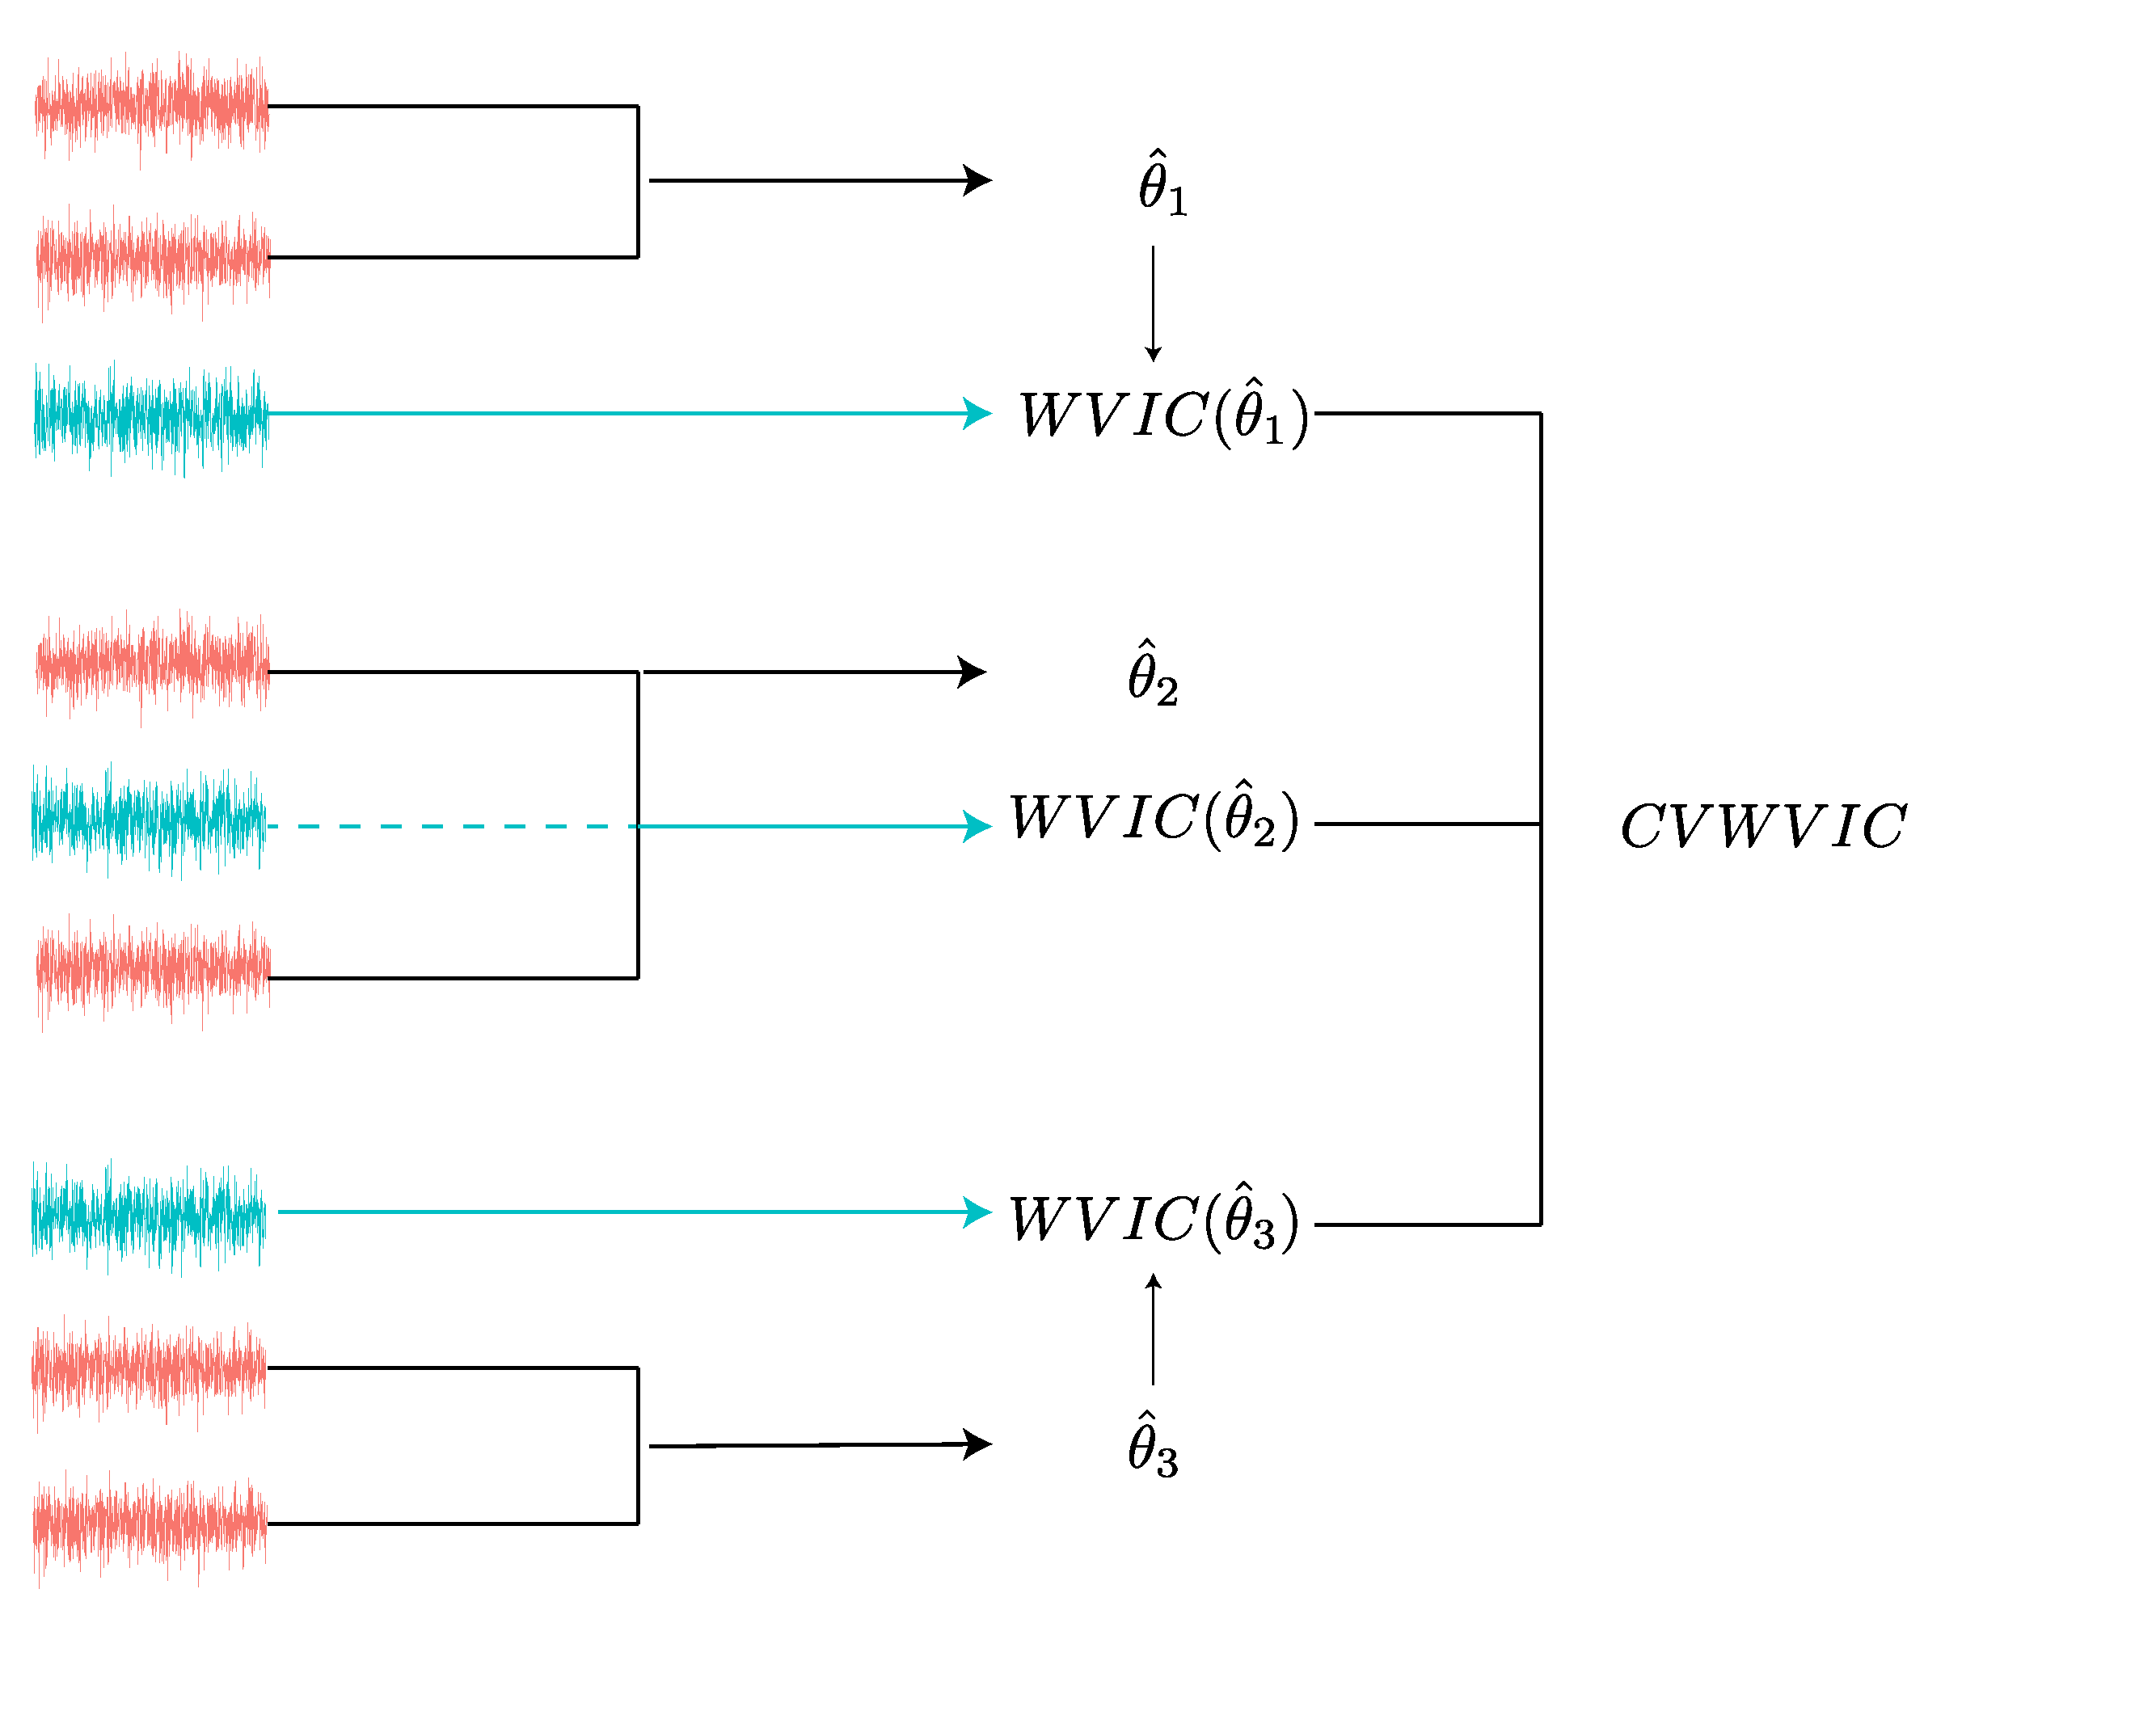
\includegraphics[scale = 0.22]{Images/cv_wvic-1.pdf}
    %\caption{Caption}
    \label{fig:appshiny}
    \end{figure}
\end{frame}

\begin{frame}{CV-WVIC}
    \begin{block}{Notation}
    \begin{itemize}
        \item We partition the $K$ replicates in two parts: the first part of size $k_1$ (with $1 \leq k_1 < K$), is used for {\color{beamer@myorange}\textbf{training purposes}},  where $M = {K\choose k_1}$ denotes the size of every possible combination $m^{(k_1)}_{i}$  for  $m = 1, \ldots, M$ and for $i = 1, \ldots, k_1$ whereas, the second part of size $k_2 = K - k_1$, for which $m^{(k_2)}_{l}$, for $l = 1, \ldots, k_2$,  defines the complement of $m^{(k_1)}_{i}$, is used for {\color{beamer@myorange}\textbf{validation purpose}}.
        \item Let $\model_{\jmath}, \, \jmath = 1, \hdots, \mathcal{J}$, denote the $\jmath^{th}$ model out of the set of $\mathcal{J}$ candidate models, with $\bm{\theta}_{\jmath} \subset \bm{\Theta}_{\jmath} \subseteq \real^{p}$ being the unknown parameter vector of $\model_{\jmath}$ and its associated parameter space.
    \end{itemize}

    \end{block}
\end{frame}

\begin{frame}{CV-WVIC: Estimation and Validation Step}
    \begin{enumerate}
        \item  We use $m_i^{k_1}$, one specific combination of the error signals replicates of size $k_1$ to estimate the parameter vector $\bm{\theta}_{\jmath}^{(m_i)}$ for the $\jmath^{th}$ model in the following manner 
%
        \begin{equation}
	        \hat{\bm{\theta}}_{\jmath}^{(m_i)} = \argmin_{\bm{\theta} \in \bm{\Theta}_{\jmath}} \sum^{k_1}_{k \in m_i^{k_1}} || \hat{\bm{\nu}}_{k} - {\bm{\nu}}(\bm{\theta}_{\jmath})||^2_{\bm{\Omega}}.
	    \label{eq:mgmwm.auto}
        \end{equation}
        \item We than compute the MGMWM objective function, evaluated at the parameter estimated in Eq. (\ref{eq:mgmwm.auto}), to deliver the $\WVIC$ computed on an independent sample $\bm{X}^{(k)}_t$ with $k \in c^{(m)}_{k_2}$:
%
\begin{equation}
	\widehat{\mathcal{C}}^{(m_l)}_{\jmath}= \sum^{k_2}_{k \in m_l^{k_2}} \| \hat{\bm{\nu}}_{k} - {\bm{\nu}}(\hat{\bm{\theta}}^{(m_i)}_{\jmath})\|_{\bm{\Omega}}^2.
	\label{eq:cvwvic1}
\end{equation}
    \end{enumerate}
\end{frame}

\begin{frame}{CV-WVIC}
    Repeating Eq. (\ref{eq:mgmwm.auto}) and (\ref{eq:cvwvic1}) for $m = 1, \ldots, M$, and computing the average $\widehat{\mathcal{C}}_{\jmath} = \frac{1}{M} \sum^M_{m = 1}\widehat{\mathcal{C}}^{(m_l)}_{\jmath}$, for each model in the $\mathcal{J}$, will allow us to select the model which minimize $\widehat{\mathcal{C}}_{\jmath}$, i.e.
\begin{equation}
	\hat{\jmath} = \argmin_{\jmath = 1,\ldots, \mathcal{J}} \widehat{\mathcal{C}}_{\jmath}.
	\label{eq:cvwvic2}
\end{equation}
\end{frame}

\begin{frame}{Case Study: The ADIS 16405 IMU}
    \begin{figure}
        \centering
        \includegraphics[scale = 0.5]{Images/adis1.pdf}
    \end{figure}
\end{frame}

\begin{frame}{Case Study: The ADIS 16405 IMU}
    \begin{figure}
        \centering
        \includegraphics[scale = 0.5]{Images/adis2.pdf}
    \end{figure}
\end{frame}

\begin{frame}{Case Study: The ADIS 16405 IMU}
    \begin{figure}
        \centering
        \includegraphics[scale = 0.5]{Images/adis3.pdf}
    \end{figure}
\end{frame}

\begin{frame}{Case Study: The ADIS 16405 IMU}
    \begin{figure}
        \centering
        \includegraphics[scale = 0.5]{Images/adis4.pdf}
    \end{figure}
\end{frame}


\begin{frame}{Web-based Platform: \href{http://mgmwm.smac-group.com/}{MGMWM}}
    \begin{figure}
        \centering
        \includegraphics[scale = 0.26]{Images/app_mgmwm.pdf}
    %\caption{Caption}
    \label{fig:appshiny2}
    \end{figure}
    
\end{frame}

\begin{frame}{Modelling Dependence between Sensors}
    \begin{figure}
        \centering
        \includegraphics[scale = 0.32]{Images/realdata_9plots.pdf}
    \end{figure}
\end{frame}

\begin{frame}{Modelling Dependence between Sensors}
    \begin{figure}
        \centering
        \includegraphics[scale = 0.64]{Images/niakette.pdf}
    \end{figure}
\end{frame}


\begin{frame}{Dynamic Calibration}
    \begin{figure}
        \centering
        \includegraphics[scale = 0.35]{Images/pilou1.png}
    \end{figure}
\end{frame}

\begin{frame}{Dynamic Calibration}
    \begin{figure}
        \centering
        \includegraphics[scale = 0.40]{Images/pilou2.png}
    \end{figure}
\end{frame}

%\footnotesize
%\frame{\printbibliography[section=1, heading = Ref]}


\begin{frame}{References}
\begin{columns}
\column{0.85\paperwidth}
\printbibliography[section=1, heading = Ref]
\end{columns}
\end{frame}

\section{Introduction to Time Series}\newrefsection

\begin{frame}{Outline}
\small
\begin{multicols}{2}
  \tableofcontents[currentsection]
\end{multicols}
\end{frame}





%\begin{frame}{GENERAL INTRO}
%TO DO
%\end{frame}

%\section{Introduction}

%\subsection{Definition \& Descriptive Analysis}

%\begin{frame}{Intro}
 %   Inertial Measurement Unit (IMU) calibration has become an important part of navigation. Most of the techniques used rely on time series analysis tools such as autocorrelation (see \cite{li2015real}) and Power Spectral Density (PSD) using Allan Variance (AV) (see \cite{elsheimy08av}). More recently \cite{guerrier2013wavelet} proposed a method based on the Generalized Method of Moments (GMM) using the Wavelet Variance (WV). 
 %   Nevertheless, it should be noted that some of the above tools are not relevant to the task of inertial sensors calibration, since the data size is far larger than what is generally used in time series. Our goal is to first introduce those classical tools and derive their statistical properties, so we can dig in the most recent techniques, which seem more appropriate for the task at hand.
%\end{frame}

\begin{frame}{Introduction}

	\begin{definition}[Time Series or TS]
	\label{def:time:series}
		A TS is a {\color{beamer@UIUCblue}\textbf{stochastic process}},(i.e. a sequence of Random Variables (RV)),  defined on a common probability space denoted as $(X_t)_{t = 1,...,T}$ (i.e. $X_1$, $X_2$, ...., $X_T$). Note that the time $t$ is not continuous and belongs to discrete index sets. Therefore, we implicitly assume that:
	\begin{itemize}
		\item $t$ is not random e.g. the time at which each observation is measured is known, and
		\item the time between two consecutive observations is constant.
	\end{itemize}
\end{definition}
	
\begin{Remark}[descriptive analysis]
In the classical time series theory, it is often useful to gain insight about a process by performing a descriptive analysis. While this approach may not be appropriate with inertial sensors, we shall briefly review it in the next few slides. 
\end{Remark}	

\end{frame}



\begin{frame}{Introduction}

\begin{Definition}[Descriptive Analysis]
	Most time series analysis starts with displaying the data as a line plot on a graph. Time on the x-axis and variable on y-axis. Such graphs are often useful to assess various properties of the data at hand.
\end{Definition}

	\begin{exampleblock}{Time Series Graph/Plot:} 
		\begin{itemize}
			\item When recording values of the same variable over an extended period of time, it is difficult to discern any trend or pattern by simply looking at the values.
			\item However, when these data points are displayed on a plot (time on $x$-axis and $X_{t}$ on $y$-axis), some features jump out.
			\item TS graph make trends easy to spot.
			\item These graphs more useful for small or moderate size data.
		\end{itemize}

	\end{exampleblock}
\end{frame}


\begin{frame}{Descriptive Analysis}
	\begin{alertblock}{Question:}
		What do we want to check for in a time series data/graph?
	\end{alertblock}
	
	\begin{block}{A possible answer:}
		\begin{itemize}
			\item Trends:
			\begin{itemize}
				\item Seasonal (e.g. business cycles)
				\item Non-seasonal (e.g. impact of economic indicators on stock returns)
				\item ``Local'' (e.g. vibrations observed before, during and after an earthquake)
			\end{itemize}
			\item Changes in the {\color{beamer@myorange} \textbf{statistical properties}}:
			\begin{itemize}
				\item Mean (e.g. economic crisis)
				\item Variance (e.g. earnings)
				\item States (e.g bear/bull in finance)
			\end{itemize}
			\item Model deviations (e.g. outliers)
		\end{itemize}
	\end{block}
\end{frame}

\subsection{Examples}

\begin{frame}{Example: Johnson and Johnson Quarterly Earnings}
	
	\begin{figure}
	    \centering
	  \includegraphics[width = 10.5cm]{Images/JJ}
	\end{figure}
	
\end{frame}

\begin{frame}{Example: Monthly Precipitation Data}
	
	\begin{figure}
	    \centering
	  \includegraphics[width = 10.5cm]{Images/precip}
	\end{figure}	
	
\end{frame}

\begin{frame}{Example: Inertial Sensor Data}
	
	\begin{figure}
	    \centering
	  \includegraphics[width = 10.5cm]{Images/imu}
	\end{figure}	
	
\end{frame}

\begin{frame}{Stochastic Processes Considered in this course}
\footnotesize
\begin{Definition}[Gaussian White Noise]
    \emph{Gaussian White Noise} (WN) with parameter $\sigma^2 \in \real^+$. This process is defined as
	%
	\begin{equation*}
		X_t  \overset{iid}{\sim} \mathcal{N}\left(0, \sigma^2 \right)
	\end{equation*}
    \label{def.WN}
    where ``iid" stands for ``independent and identically distributed". 
\end{Definition}

\begin{Definition}[Quantization Noise]
    \emph{Quantization Noise} (QN) with parameter $Q^2 \in \real^+$. This process has a PSD of the form
	%
	\begin{equation*}
		S_{X}(f) = 4 Q^2 \sin^2 \left( \frac{\pi f}{\Delta t} \right) \Delta t, \;\; f < \frac{\Delta t}{2}.
	\end{equation*} 
	\label{def.QN}
\end{Definition}

    \begin{Definition}[Drift]
\emph{Drift} (DR) with parameter $\omega \in \Omega$ where $\Omega$ is either $\real^+$ or $\real^-$. This process is defined as $X_t = \omega t$.
\label{def.drift}
\end{Definition}

\end{frame}

\begin{frame}{Stochastic Processes Considered in this course}
\small

\begin{Definition}[Random walk]
     \emph{Random walk} (RW) with parameter $\gamma^2 \in \real^+$. This process is defined as
		%
		\begin{equation*}
			X_t = X_{t-1} + \epsilon_t \;\; \text{where}\;\; \epsilon_t  \overset{iid}{\sim} \mathcal{N}\left(0, \gamma^2 \right)\;\; \text{and}\;\; X_0 = 0.
		\end{equation*}
		\label{def.RW}
\end{Definition}

\begin{Definition}[Auto-Regressive]
\emph{Auto-Regressive Process of Order 1} (AR1) process with parameter $\phi \in (-1, +1)$ and $\upsilon^2 \in \real^+$. This process is defined as
	%
	\begin{equation*}
      X_t = \phi X_{t-1} + Z_t, \;\;\; Z_t \simiid \mathcal{N}(0,\upsilon^2).
	\end{equation*}
	\label{def.AR1}
\end{Definition}

\end{frame}



\begin{frame}{Stochastic Processes Considered in this course}
\small


\begin{Definition}[Gauss Markov]
\label{def.GM}
\emph{Gauss Markov Process of Order 1} (GM) process with parameter $\beta \in \real$ and $\sigma_G^2 \in \real^+$. This process is defined as
	%
	\begin{equation*}
      X_t = \exp(-\beta \Delta_t) X_{t-1} + Z_t, \;\;\; 
      Z_t \simiid \mathcal{N}(0,\sigma^2_{G}(1-\exp(-2\beta\Delta t)))
	\end{equation*}
	%
	where $\Delta t$ denotes the time between $X_t$ and $X_{t-1}$.
\end{Definition}

\begin{Remark}[GM and AR1]
A GM process is a one-to-one reparametrization of an AR1 process. In this course, we shall only discuss AR1 processes but all results remain valid for GM processes.
\end{Remark}

\end{frame}


\begin{frame}{Stochastic Processes Considered in this course}
    \normalsize
    \begin{Definition}[Composite stochastic processes]
    \label{def:composite}
    A composite stochastic process is a sum of latent processes. In this course, we will always assume that these latent processes are independent.
    \end{Definition}
    
    \begin{exampleblock}{Example:}
    The composite stochastic process: ``2*AR1 + WN'' is given:
\begin{equation*}
    \begin{aligned}
        Y_t &= \phi_1 Y_{t-1} + Z_t, \;\;\; Z_t \simiid \mathcal{N}(0,\upsilon_1^2)\\
         W_t &= \phi_2 W_{t-1} + U_t, \;\;\; U_t \simiid \mathcal{N}(0,\upsilon_2^2)\\
         Q_t &\simiid \mathcal{N}(0,\sigma^2)\\
         X_t &= Y_t + W_t + Q_t,
    \end{aligned}
\end{equation*}
%
where {\color{beamer@myorange}\textbf{only}} $(X_t)$ is observed.
    \end{exampleblock}
\end{frame}



\subsection{Measuring Dependence}
%\{Introduction}

\begin{frame}{Main purpose of TS analysis: Forecasting}
	\small
	\begin{block}{ }
		\begin{itemize}
			\item {\color{beamer@UIUCblue}\textbf{Forecasting}} is one of the main purpose of time series analysis. The question can be described as: if $(X_t)_{t = 1, ..., T}$ is an identically distributed sequence but is {\color{beamer@myorange}\emph{not independent}}, what is the ``best'' predictor for ${X}_{T+h}$ for $h > 0$ (i.e. an estimator of $\mathbb{E}[X_{T+h}| X_T,...]$)? 
			\item \emph{A simple answer is that it depends on the ``dependence'' between $X_{1},\hdots,X_{T}$!}
			\item How could we measure this dependence?
			\item A first step is to extend the notation of covariance and correlation to time dependent sequences. We will refer to these notions as {\color{beamer@UIUCblue}\textbf{autocovariance}} and {\color{beamer@UIUCblue}\textbf{autocorrelation}}.
			\item The notion of autocovariance is an important one in time series analysis as it is closely linked to the concept of stationarity. Informally speaking, the latter creates a framework in which averages are ``meaningful'' (we will come back to this).
		\end{itemize}
	\end{block}
\end{frame}
	
\begin{frame}{Review of Independence and Dependence}
		\small
		\begin{Definition}[Independence of two events]
		   Two events $A$ and $B$ are independent if 
		       $\mathbb{P}(A \cap B) = \mathbb{P}(A)\mathbb{P}(B)$.
		   %
		\end{Definition}
		
		\begin{Definition}[Independence of two random variables]
		  Two random variables $X$ and $Y$ with Cumulative Distribution Functions (CDF) $F_X(x)$ and $F_Y(y)$ (respectively) are {\color{beamer@UIUCblue} \textbf{independent}} if and only if their joint CDF $F_{X,Y}(x,y)$ is such that $
		      F_{X,Y}(x,y) = F_{X}(x) F_{Y}(y)$.
		\end{Definition}
		
		\begin{Definition}[iid sequence]
		The sequence $X_{1},X_{2},\hdots,X_{T}$ is said to be {\color{beamer@UIUCblue} \textbf{iid}} if and only if
		%
		\begin{equation*}
		    \mathbb{P}(X_{i}<x) = \mathbb{P}(X_{j}<x) \;\; \forall x \in \real, \forall i,j \in \{1,\ldots,T\},  \;\; \text{and}
		\end{equation*}
		%
		%
		\begin{equation*}
		    \mathbb{P}(X_{1}<x_{1},X_{2}<x_{2},\hdots,X_{T}<x_{T})=\mathbb{P}(X_{1}<x_1)...\mathbb{P}(X_{T}<x_T), 
		\end{equation*}
		%
		for any $T\geq2$ and $x_1, ..., x_T \in \real$.
		\end{Definition}
		

\end{frame}


%\subsection{Autocovariance}

\begin{frame}{Measuring (linear) dependence}
\footnotesize
	{\textbf{\color{beamer@myorange}Dependence between $T$ RV is difficult to measure at one shot!}} So we consider just two random variables, $X_{t}$ and $X_{t+h}$. Then, one common (linear) measure of dependence is the covariance between $X_{t}$ and $X_{t+h}$, which is defined below.
	
	\begin{Definition}[AutoCovariance]
	\label{definition:autocov}
		The covariance between $X_{t}$ and $X_{t+h}$, defined as the {\color{beamer@myorange}\emph{AutoCovariance}} or simply ACV,  is denoted using the function $\gamma_X(t, t+h)$, i.e.
%
        \begin{equation*}
            \gamma_X(t, t+h) \equiv	\text{Cov}(X_{t},X_{t+h})= 	\mathbb{E}(X_{t}X_{t+h})-	\mathbb{E}(X_{t})	\mathbb{E}(X_{t+h}),
        \end{equation*}
%				
where
%
        \begin{equation*}
            \begin{aligned}
                \mathbb{E}(X_{t}) &= \int_{-\infty}^{\infty}x \, f(x) dx \\
		        \mathbb{E}(X_{t},X_{t+h}) &= \int_{-\infty}^{\infty}\int_{-\infty}^{\infty}x_{1}x_{2} f(x_{1},x_{2}) dx_{1}dx_{2},
            \end{aligned}
        \end{equation*}
        %
        where $f(x_{1},x_{2})$ denotes the joint density of $X_{t}$ and $X_{t+h}$.
	\end{Definition}
\end{frame}


\begin{frame}{Measuring (linear) dependence}
	
	\begin{Remark}[Scale dependence]
	Just as any covariance, the $\gamma_X(t, t+h)$ is ``scale dependent'' and therefore $\gamma_X(t, t+h)\in\real$.
				\begin{itemize}
					\item If $\mid \gamma_X(t, t+h) \mid$ is ``close'' to 0, then they are ``less dependent''.
					\item If $\mid \gamma_X(t, t+h) \mid$ is ``far'' from 0, $X_{t}$ and $X_{t+h}$ are ``more dependent''.
				\end{itemize}
	\end{Remark}
	
	\begin{Remark}[ACV and independence]
	$\gamma_X(t, t+h)=0$ does not imply $X_{t}$ and $X_{t+h}$ are independent. However, if $X_{t}$ and $X_{t+h}$ are joint normally distributed then $\gamma_X(t, t+h)=0$ implies that $X_{t}$ and $X_{t+h}$ are independent.
	\end{Remark}
	
\end{frame}

%\subsection{Autocorrelation}

\begin{frame}{Measuring (linear) dependence}
	\small
	A measure of dependence related to the ACV is the autocorreation. This is arguably the most commonly used metric in time series analysis.
	
	\begin{Definition}[Autocorrelation]
		The correlation between $X_{t}$ and $X_{t+h}$ is defined as the {\color{beamer@myorange}\emph{autocorrelation}} or simply ACF and is denoted using the function $\rho_X(t, t+h)$, i.e.
		%
		\begin{equation*}
			\rho_X(t,t+h) = \corr(X_{t},X_{t+h}) = \frac{\cov(X_{t},X_{t+h})}{\sqrt{\var(X_{t})} \sqrt{\var(X_{t+h})}}
		\end{equation*}
	\end{Definition}
	
	\begin{Remark}[Scale invariance]
	Just as any correlation, $\rho_X(t,t+h)$ is scale free. Moreover, if $\rho_X(t,t+h)$ is ``close'' to $\pm 1$ then this implies that there is ``strong'' (linear) dependence between $X_{t}$ and $X_{t+h}$.
	\end{Remark}
\end{frame}

\begin{frame}{Measuring (linear) dependence}
\footnotesize
	\begin{Remark}[Notation]
	The notation $\gamma_X(t, t+h)$ and $\rho_X(t, t+h)$ is often simplified to  $\gamma(t, t+h)$ and $\rho(t, t+h)$ when not ambiguous (i.e. only one time series is considered). 
	\end{Remark}
	
\begin{Remark}[Linear dependence and real dependence]
	Covariance and correlation measure linear dependence. They are less helpful to measure monotonic dependence and they are much less helpful to measure nonlinear dependence. Nonlinear measures of dependence exist but we will not discuss this subject in this class. Here is an example:
\end{Remark}

%	\begin{figure}
%	    \centering
%	  \includegraphics[width = 6.75cm]{Images/Cor}
%	\end{figure}
%\end{frame}

%\begin{frame}{Correlation == Causation?}
%	\footnotesize
\begin{Remark}[Causation]
    Correlation {\color{beamer@myorange} \emph{does NOT}} imply causation. For example, if $\rho(t, t+h) \neq 0$ it does not imply that $X_t \to X_{t+h}$ is causal. Actually, real causation doesn't exist in Statistics but there exist approximated metric to measure this concept such as Granger causality (see \cite{granger1969investigating}). This idea is clearly illustrated in the image below. 
\end{Remark}

%	\begin{figure}
%	    \centering
%	  \includegraphics[width = 6cm]{Images/corr_cat}
%	\end{figure}
	
\end{frame}


%\section{Stationarity}

%\subsection{Introduction}

\subsection{Stationarity}

\begin{frame}{Estimation of in the context of time series}
	\small
	\begin{exampleblock}{Motivation:}
		Consider the simple (but strange!) model:
		%
		\begin{equation*}
			X_t  \sim \mathcal{N} \left(0, Y_t^2\right) \;\; \text{where $Y_t$ is unobserved and such that} \;\; Y_t  \stackrel{iid}{\sim} \mathcal{N} \left(0, 1\right).
		\end{equation*}
		%
		In this case, it is clear that the estimation of $\var(X_t)$ is difficult (in fact $X_t^2$ is your best guess!) since only $X_t$ is useful to estimate $\var(X_t)$. This process is an example of a {\color{beamer@UIUCblue}\textbf{non-stationary process}} (we will see why in the next slides). On the other hand, if we consider the {\color{beamer@UIUCblue}\textbf{stationarity process}} such as:
		%
		\begin{equation*}
			X_t = \theta W_{t-1} + W_t \;\;\; \text{where} \;\;\;  W_t  \stackrel{iid}{\sim} \mathcal{N} \left(0, 1\right).
		\end{equation*}
		%
		Then, one can guess that a natural estimator of $\var(X_t)$ is simply $\hat{\sigma}^2 = \frac{1}{T} \sum_{i = 1}^T X_i^2$, 
		because our hope is that averages are ``{\color{beamer@myorange}\textbf{meaningful}}'' for such processes. In the next slides, we will formalize this idea through the concepts of stationarity.
	\end{exampleblock}
\end{frame}


\begin{frame}{Strong and Weak Stationarity}
\small
There exist two forms of stationarity, which are defined below:

	\begin{Definition}[Strong Stationarity]
		The joint probability distribution of $(X_{t})_{t \in \mathbb{N}}$ is invariant under a shift in time, i.e.
			%
			\begin{equation*}
				\mathbb{P}(X_{t}\leq x_{1},\hdots,X_{t+k}\leq x_{k}) =
						\mathbb{P}(X_{t+h}\leq x_{1} ,\hdots,X_{t+h+k}\leq x_{k})
			\end{equation*}
			%
		for any time shift $h$ and any $x_{1},x_{2},\cdots,x_{k}$ belong to the domain of $X_t,\cdots,X_{t+k}$ and $X_{t+h},\cdots,X_{t+h+k}$. %respectively.
	\end{Definition}
	
	\begin{Definition}[Weak Stationarity]
		The mean and autocovariance of the stochastic process are finite and invariant under a shift in time, i.e.
		%
		\begin{equation*}
			\begin{aligned}
				\mathbb{E}\left[X_t\right] &= \mu < \infty,\\
				\mathbb{E}\left[X_t^2\right]  &= \mu_2 < \infty,\\
				\cov(X_{t},X_{t+h})&= \cov(X_{t + k},X_{t+h + k})
				= \gamma( h ).
			\end{aligned}
		\end{equation*}
	\end{Definition}
	

\end{frame}


%\subsection{Remarks}

\begin{frame}{Strong and Weak Stationarity}
	\small
    \begin{block}{Why does stationarity matter?}
    The stationarity of ${X_{t}}$ is important because it provides a framework in which averaging makes sense. Unless properties like mean and covariance are either {fixed} or ``evolve'' in a known manner, the concept of averaging is essentially meaningless.
    \end{block}
    
    \begin{Remark}[Implication on the ACV and ACF]
    \label{rem:ACF:stab}
    If a process is weakly stationary or strongly stationary and $\cov(X_{t},X_{t+h})$ exist for all $h \in \mathbb{Z}$. Then we have the ACV and ACF only depends on the lag between observations, i.e.
    %
    \begin{equation*}
        \begin{aligned}
            \gamma(t, t+h) &= \cov(X_{t},X_{t+h})= \cov(X_{t + k},X_{t+h + k}) = \gamma(t+k, t+h+k) = \gamma(h),\\
            \rho(t, t+h) &= \corr(X_{t},X_{t+h})= \corr(X_{t + k},X_{t+h + k}) = \rho(t+k, t+h+k) = \rho(h).
        \end{aligned}
    \end{equation*}
    %
    \end{Remark}
\end{frame}
  
  \begin{frame}{Strong and Weak Stationarity}
	\footnotesize  
	
\begin{Remark}[Properties of the ACV and ACF]
Remark \ref{rem:ACF:stab} implies that the ACV and ACF have the following properties:
    \begin{itemize}
			\item $\gamma(0) = \var \left[X_t\right] \geq 0$ and $\rho(0) = 1$.
			\item $\gamma(h) = \gamma(-h)$ and $\rho(h) = \rho(-h)$ (therefore they are both even functions).
			\item $|\gamma(h)|  \leq \gamma(0)$ and $|\rho(h)|  \leq 1 $ for all $ h\in \mathbb{Z}$.
			\end{itemize}
		\end{Remark}	

The first two properties are direct for the properties of the covariance and correlation (i.e. $\cov(X,X) = \var(X)$ and $\cov(X,Y) = \cov(Y,X)$). However, the third property is less obvious and is a consequence of the Cauchy-Schwarz inequality, i.e.
%
\begin{equation}
    \label{eq:cauchy_sch}
     \mathbb{E}^2\left[XY\right] \leq \mathbb{E}\left[X^2\right] \mathbb{E}\left[Y^2\right].
\end{equation}
%
Using (\ref{eq:cauchy_sch}), we have
%
\begin{equation*}
    \begin{aligned}
             \gamma(h)^2 &= \left(\cov\left(X_t, X_{t+h}\right)\right)^2 = \left( \mathbb{E}\left[\left(X_t - \mu\right)\left(X_{t+h} - \mu\right)\right] \right)^2\\
             &\leq \mathbb{E}\left[\left(X_t - \mu\right)^2\right] \mathbb{E}\left[\left(X_{t+h} - \mu\right)^2\right] = \gamma(0)^2,
    \end{aligned}
\end{equation*}
%
which verifies the last properties.
\end{frame}

\begin{frame}{Remarks: Strong and Weak Stationarity}

	\begin{Remark}
	\label{rem:stati}
	\textbf{Neither type of stationarity implies the other one}. This is being illustrated in the two examples presented in \ref{app:strong:weak} $\;$ \hyperlink{app:strong:weak}{\beamergotobutton{Go to \ref{app:strong:weak}}}. Note however that if $X_{t}$ is Normal (Gaussian) with $\sigma^2=\var(X_{t})<\infty$, then weak stationarity implies strong stationarity.
	\end{Remark}
	
	\begin{Remark}
	\label{rem:verif}
	From the definition of (weak) stationarity, it is easy to see that a WN or a QN processes is stationary while a RW process is not. The stationarity of an AR1 (or GM) is less obvious. In fact, an AR1 is stationary if $|\phi| < 1$. The derivation of this property is given in \ref{app:ar1:stat:example} $\;$ \hyperlink{app:strong:weak}{\beamergotobutton{Go to \ref{app:ar1:stat:example}}}.
	\end{Remark}
\end{frame}

%\subsection{Linear Processes}
  
\begin{frame}{Linear Processes}
\footnotesize

\begin{Definition}[Linear Processes]
\label{def:linear:process}
A stochastic process $(X_t)$ is said to be a linear process if it can be expressed as a linear combination of an iid sequence (which here is Gaussian for convenience), i.e.:
%
\[{X_t} = \mu + \sum\limits_{j =  - \infty }^\infty  {{\psi _j}{W_{t - j}}} \]
%
where $W_t \simiid \mathcal{N}(0, \sigma^2)$ and $\sum\limits_{j =  - \infty }^\infty  {\left| {{\psi _j}} \right|}  < \infty$.

\end{Definition}

\begin{Remark}[Properties of linear processes]
All linear processes are stationary and such that:
%
\[\begin{aligned}
\mathbb{E}[X_t] &= \mu, \\
\gamma(h) &= \sigma^2\sum\limits_{j =  - \infty }^\infty  {{\psi _j}{\psi _{h + j}}}.
\end{aligned}\]
\end{Remark}
\end{frame}


\begin{frame}{Linear Processes}
\scriptsize

\begin{Remark}[Convergence of linear processes]
The latter condition $\sum\limits_{j = - \infty }^\infty {\left| {{\psi _j}} \right|} < \infty$ is required to ensure that the series has a limit and is related to the absolutely summable covariance structure (defined below).
\end{Remark}


\begin{Definition}[Absolutely summable covariance structure]
\label{def:abs:sum}
A process $(X_t)$ is said to have an absolutely summable covariance structure if $\sum\limits_{h = - \infty }^\infty {\left| \gamma_X(h) \right|} < \infty$.
\end{Definition}

\begin{Remark}[All linear process have an absolutely summable covariance structure]
Interestingly, the condition $\sum\limits_{j = - \infty }^\infty {\left| {{\psi _j}} \right|} < \infty$ is actually stronger than $\sum\limits_{h = - \infty }^\infty {\left| \gamma_X(h) \right|} < \infty $. Indeed, we have that
%
\begin{equation*}
    \sum\limits_{h = - \infty }^\infty {\left| \gamma_X(h) \right|} \leq 2 \gamma(0) \left( \sum\limits_{j = - \infty }^\infty {\left| {{\psi _j}} \right|} \right)^2 < \infty.
\end{equation*}
%
\end{Remark}

\end{frame}

\subsection{Fundamental Representations}

\begin{frame}{A Fundamental Representation}
    
\begin{alertblock}{A Fundamental Representation}
Autocovariances and autocorrelations also turn out to be very useful tools as they are one of the \textit{fundamental representations of time series}.\\[0.2cm]

If we consider a \underline{zero mean normally distributed process}, it is clear that its joint distribution is fully characterized by the autocovariances $\mathbb{E}[X_t X_{t+h}]$ since the joint probability density only depends on these covariances.\\[0.2cm]

Once we know the autocovariances we know everything there is to know about the process and therefore: \textbf{if two processes have the same autocovariance function, then they are the same process}.
\end{alertblock}

\end{frame}

\begin{frame}{Another Fundamental Representation}
    
\begin{alertblock}{Fundamental Representation: the Power Spectral Density}
For the same processes considered in the previous slide, another fundamental representation of a time series is given by the Power Spectral Density (PSD) which can be defined as
%
\begin{equation*}
    S_X(f) = \int_{- \infty}^{\infty} \gamma_{X}(h)\,e^{-ifh}dh,
\end{equation*}
%
where $f$ is a frequency. Hence, the PSD is a Fourier transform of the autocovariance function which describes the variance of a time series over frequencies (with respect to lags $h$).\\[0.2cm]

Given that the definition of the PSD, as for the autocovariance function, once we know the PSD we know everything there is to know about the process and therefore: \textbf{if two processes have the same PSD, then they are the same process}.
\end{alertblock}

\end{frame}





%\section{Estimation}
% linear process???
%\subsection{Expected Value}

\begin{frame}{Estimation Problems with Dependent Data}
\small
Estimation in the context of time series is not as straightforward as in the iid case. In order to ``warm-up", let us start with the easiest case: the empirical mean.

	\vspace{0.25cm}
		Let $(X_t)$ be a stationary time series, therefore we have that $\mu_t = \mathbb{E}[X_t] = \mu$ and the value of $\mu$ can be estimated by the sample mean, i.e.
		%
		\begin{equation*}
			\bar{X} = \frac{1}{T} \sum_{t = 1}^T X_t.
		\end{equation*}
		%
		Using the properties of stationary process we have that:
		%
		\begin{equation}
			\var \left(\bar{X}\right) = \frac{1}{T^2} \cov \left( \sum_{t = 1}^T X_t, \sum_{s = 1}^T X_s \right) = \frac{\gamma(0)}{T} \sum_{h = -T}^T \left(1 - \frac{|h|}{T}\right) \rho(h).
			\label{eq.varxbar}
		\end{equation}
		%
The derivation of (\ref{eq.varxbar}) is instructive and is given in \ref{app:deriv:var:bar} $\;$ \hyperlink{app:strong:weak}{\beamergotobutton{Go to \ref{app:deriv:var:bar}}}. Moreover, some simulation-based and analytical methods to estimate $\var \left(\bar{X}\right)$ are discussed in \ref{app:var:xbar:in:practice} $\;$ \hyperlink{app:var:xbar:in:practice}{\beamergotobutton{Go to \ref{app:var:xbar:in:practice}}}.
\end{frame}


%\subsection{Autocovariance \& Autocorrelation}

\begin{frame}{Estimation of $\gamma(h)$ and $\rho(h)$}
	\footnotesize
	We define here the ``classical'' estimator of $\gamma(h)$ and $\rho(h)$ as the sample autocovariance and autocorrelation functions. In the following section, we shall study the properties of these estimators:
	
	\begin{Definition}[Sample autocovariance function]
	\label{def:sample:auto:cov}
		The {sample autocovariance function} is defined as
		%
		\begin{equation*}
			\hat{\gamma}(h) = \frac{1}{T} \sum_{t = 1}^{T-h} \left(X_{t} - \bar{X}\right) \left(X_{t+h} - \bar{X}\right)
		\end{equation*}
		%
		with $\hat{\gamma}(h) = \hat{\gamma}(-h)$ for $h = 0, 1, ..., k$, where $k$ is a fixed integer.
	\end{Definition}
	
	\begin{Definition}[Sample autocorrelation function]
	\label{def:sample:auto:cor}
		The {sample autocorrelation function} is defined as
		$\hat{\rho}(h) = \frac{\hat{\gamma}(h)}{\hat{\gamma}(0)}$,
		%
		with $\hat{\rho}(h) = \hat{\rho}(-h)$ for $h = 0, 1, ..., k$, where $k$ is a fixed integer.
	\end{Definition}
	
\end{frame}

%\footnotesize
%\frame{\printbibliography[section=2, heading = Ref]}

\section{Properties of Estimators}\newrefsection

\begin{frame}{Outline}
\small
\begin{multicols}{2}
  \tableofcontents[currentsection]
\end{multicols}
\end{frame}

\subsection{Extremum Estimators}

\begin{frame}{Statistical Estimators}
\footnotesize

In this section, we shall present an introduction to the study of the properties of statistical estimators. We will mainly focus on asymptotic properties and start by consider a general class of estimators.
\vspace{0.15cm}

	\begin{Definition}[Extremum Estimator]
	\label{def:extrem:est}
	Many estimators have a \textbf{{\color{beamer@UIUCblue}common structure}}, which is often useful to study their asymptotic properties. One structure or framework is the class of estimators that maximize some objective function, referred to as extremum estimators, which can can be defined as follows:
		%
		\begin{equation}
			{\hat{\btheta} \equiv \argmax_{\btheta \in \bTheta} \; \hat{Q}_n (\btheta),}
			\label{eq:extrem:estim}
		\end{equation}
		%
		where $\btheta$ and $\bTheta$ denote, respectively, the parameter vector of interest and its set of possible values.
	\end{Definition}
	
	\begin{exampleblock}{Remark:}
		The vast majority of statistical estimators can be represented as extremum estimator. This is for example for the case for least squares, maximum likelihood or (generalized) method of moment estimators.
	\end{exampleblock}
\end{frame} 

\begin{frame}{Example: Least Squares Estimator}
	Consider the linear model $\y = \X \bbeta_0 + \bvarep$ where $\X \in \real^{n \times p}$ is a full-ranked constant matrix, $[\bvarep]_i \simiid  \left({0}, \sigma^2_{\bvarep} \right)$ and $\bbeta \in {\mathcal{B}} \subseteq \real^p$. Let $\hat{\bbeta}$ denote the Least Squares Estimator (LSE) of $\bbeta_0$, i.e.
		%
		\begin{equation*}
			\hat{\bbeta} = \left(\X^T \X \right)^{-1} \X^T \y. 
		\end{equation*}
		%
		Moreover, this estimator is an extremum estimator since it can expressed as:
		%
		\begin{equation*}
			\hat{\bbeta} = \argmax_{\bbeta \in \mathcal{B}} \; -||\y - \X \bbeta ||_2^2,
		\end{equation*}
		% 
		similarly to our definition given in (\ref{eq:extrem:estim}). \hfill \tikzcircle[black, fill=black]{3pt}	
\end{frame}

\begin{frame}{Example: Maximum Likelihood Estimator}
	
	Let $Z_1, \ldots, Z_n$ be an iid sample with pdf $f(z|\bm{\theta}_0)$. The Maximum Likelihood Estimator (MLE) is given by
	%
	\begin{equation}
	    \hat{\btheta} = \argmax_{\btheta \in \bTheta} \; \frac{1}
	{n} \sum_{i = 1}^{n} \log\left[f\left(z_i| \btheta\right)\right].
	\label{chap1:eq:example:1}
	\end{equation}
	%
	Therefore, the MLE can be seen as an example of extremum estimator with
	%
	\begin{equation*}
		\hat{Q}_n(\btheta) = \frac{1}
		{n} \sum_{i = 1}^{n} \log\left[f\left(z_i| \btheta\right)\right].
	\end{equation*}
	%
	\hfill \hfill \tikzcircle[black, fill=black]{3pt} \vspace{0.5cm}
	
	\small
	\textbf{{\color{beamer@UIUCblue}Remark:}} In (\ref{chap1:eq:example:1}) we are actually using a {\color{beamer@myorange}\emph{normalized}} log-likelihood instead of the actual log-likelihood. This has (in the vast majority of cases) no impact on the estimator but the normalized form is more convenient to use when we let $n \to \infty$.
	
\end{frame}


\begin{frame}{Example: Generalized Method of Moment}
	\small
	
		Consider the same iid sample as in the previous example and suppose that there is a ``moment function'' vector $\g(z | \btheta)$ such that $\mathbb{E}[\g (z | \btheta_0)] = 0$. Then, a possible estimator of $\btheta_0$ is
		%
		\begin{equation}
			\hat{\btheta} = \argmax_{\btheta \in \bTheta} \; - \left[\frac{1}{n} \sum_{i = 1}^n \g(z_i | \btheta) \right]^T \widehat{\W} \left[\frac{1}{n} \sum_{i = 1}^n \g(z_i | \btheta) \right],
			\label{eq:gmm}
		\end{equation}
		%
		where $\widehat{\W}$ is an positive definite matrix of appropriate dimension. Such estimators are called {\color{beamer@myorange}Generalized Method of Moments (GMM) estimators}. They belong to the class of extremum estimators. \hfill \hfill \tikzcircle[black, fill=black]{3pt} \vspace{0.5cm}
		
		\footnotesize
		\textbf{{\color{beamer@UIUCblue}Remark:}} Instead of (\ref{eq:gmm}) we will often consider an alternative (but equivalent) definition of such estimator, i.e.
		%
		\begin{equation*}
				\hat{\btheta} = \argmax_{\btheta \in \bTheta} \; - || \hat{\bm{\mu}} - \bm{\mu}(\bm{\theta}) ||_{\widehat{\W}}^2,
		\end{equation*}
		%	
		where $|| \mathbf{x} ||_{\mathbf{A}}^2 = \mathbf{x}^T \mathbf{A} \mathbf{x}$, and where $\hat{\bm{\mu}}$ and $\bm{\mu}(\bm{\theta})$ denote, respectively, the empirical and model based moments.
\end{frame}

\begin{frame}[label = {exampleGMM}]{Example: A simple GMM Estimator}
	\label{ex:gmm}
	\footnotesize
	Let $Z_i \simiid \mathcal{N}(\mu_0, \sigma^2_0)$ and $\btheta_0 = (\mu_0, \sigma_0^2)^T$. Suppose we wish to estimate $\btheta_0$ by matching the first three empirical moments with their theoretical counterparts. In this case, a reasonable moment function or condition defining a GMM estimator is given by:
	%
	\begin{equation*}
		\g (Z | \btheta) = \begin{bmatrix}
	 Z - \mu\\
	 Z^2 - \left(\mu^2 + \sigma^2\right)\\
	 Z^3 - \left(\mu^3 + 3 \mu \sigma^2\right)
	 \end{bmatrix}.
	\end{equation*}
	%
	However, it can be noticed that $\frac{1}{n} \sum_{i=1}^n \g (Z_i | \btheta) = \hat{\bgamma} - \bgamma(\btheta)$, where $\hat{\bgamma}$ and $\bgamma(\btheta)$ denote, respectively, the empirical and model-based moments, i.e.
	%
	\begin{equation*}
		\hat{\bgamma} = \frac{1}{n}  \sum_{i = 1}^n 
	\begin{bmatrix}
	  Z_i\\
	 Z_i^2\\
	 Z_i^3\\
	 \end{bmatrix}, \;\;\;\;
		\bgamma(\btheta) = 	\begin{bmatrix}
			 \mu\\
			\mu^2 + \sigma^2\\
			\mu^3 + 3 \mu \sigma^2
	 		 \end{bmatrix}.
	\end{equation*}

	Then, we can write our GMM estimator of $\btheta_0$ as:
	%
	\begin{equation}
		\hat{\btheta} = \argmin_{\btheta \in \bTheta} \; || \hat{\bgamma} - \bgamma (\btheta) ||_{\widehat{\W}}^2 = \argmax_{\btheta \in \bTheta} \;  - || \hat{\bgamma} - \bgamma (\btheta) ||_{\widehat{\W}}^2.
		\label{eq:gmm:form2}
	\end{equation}
	%
	 \hfill \tikzcircle[black, fill=black]{3pt}
\end{frame}

\subsection{Consistency}
\begin{frame}{Consistency of Statistical Estimators}
	
		In the next slides we will discuss the conditions for the consistency of extremum estimator, which is often denoted as $\hat{\btheta} \xmapsto[\;\;\;\;\; ]{\mathcal{P}} \btheta_0$. We start by defining consistency. \vspace{0.5cm}
		
		\begin{alertblock}{Definition: Consistency}
			The estimator $\hat{\btheta}$ is said to be consistent if it converges in probability to $\btheta_0$, i.e.
			%
			\begin{equation*}
				\lim_{n \to \infty} \Pr \left(|| \hat{\btheta} - \btheta_0 ||_2 \geq \varepsilon \right) = 0,
			\end{equation*}
			%
			for all $\varepsilon > 0$. 
		\end{alertblock}
		
\end{frame}

\begin{frame}{Consistency - Interpretation}
	
	\begin{exampleblock}{Interpretation:}
		In Layman's term consistency simply means that if $n$ is ``large enough'' $\hat{\bm{\theta}}$ will be {\color{beamer@myorange}\textbf{arbitrarily close to $\bm{\theta}_0$}} (i.e. inside of an hypersphere of radius $\varepsilon$ centered at $\bm{\theta}_0$). This also means the procedure (i.e. our estimator) based on unlimited data will be able to identify the underlying truth (i.e.  $\bm{\theta}_0$).
	\end{exampleblock}
	
	\vspace{-0.1cm}
	\begin{figure}
	    \centering
	  \includegraphics[width = 7.5cm]{Images/consistency}
	\end{figure}
\end{frame}


\begin{frame}{Related Theorems}

Consistency is often proven using the following two important results.

	\begin{Theorem}[Weak Law of Large Number]
	\label{thm:wlln}
		Suppose $X_i$ are iid random variables with finite mean $\mu$ (i.e. $\mathbb{E}[X_i] = \mu$) and finite variance. Let $\bar{X}_n = \frac{1}{n} \sum_{i = 1}^n X_i$, then $\bar{X}_n \xmapsto[\;\;\;\;\; ]{\mathcal{P}} \mu$.
		\label{theo.wll}
	\end{Theorem}
	
	\begin{Theorem}[Continuous Mapping Theorem]
	\label{thm:continuousmap}
		Suppose $Y_n \xmapsto[\;\;\;\;\; ]{\mathcal{P}} \mu$, then $g(Y_n) \xmapsto[\;\;\;\;\; ]{\mathcal{P}} g(\mu)$ if $g(\cdot)$ is a continuous function.
	\end{Theorem}
	
\vspace{0.5cm} 
A simple example on the consistency is presented in \ref{app:consist:simple} $\;$ \hyperlink{app:consist:simple}{\beamergotobutton{Go to \ref{app:consist:simple}}}.  
\end{frame}


\begin{frame}{Consistency of Extremum Estimators}
	\footnotesize
	
	When considering real-life problems the approach based on Theorem \ref{thm:wlln} presented in \ref{app:consist:simple} is in general not flexible enough and we generally rely on the results such the one presented below.
	
	\begin{Theorem}[Consistency of Extremum Estimators]
	\label{thm:consist}
		\footnotesize
			If there is a function ${Q}_0 (\btheta)$ such that:
			%
			\begin{enumerate}
				\setlength{\itemindent}{0.06in}
				\item[(C.1)] ${Q}_0 (\btheta)$ is uniquely maximized in $\btheta_0$,
				\label{theo:consist:cond:unique:max}
				\item[(C.2)] $\bTheta$ is compact\footnote{Compact means that $\bTheta$ is both closed (i.e. containing all its limit points) and bounded (i.e. all its points are within some fixed distance of each other).},
				\label{theo:consist:cond:compact}
				\item[(C.3)] ${Q}_0 (\btheta)$ is continuous in $\btheta$,
				\label{theo:consist:cond:continuous}
				\item[(C.4)] $\hat{Q}_n (\btheta)$ converges uniformly in probability to $Q_0 (\btheta)$\footnote{$\hat{Q}_n (\btheta)$ is said to converges uniformly in probability to $Q_0 (\btheta)$ if $\sup_{\btheta \in \bTheta} \; |\hat{Q}_n (\btheta) - {Q}_0 (\btheta)| \xmapsto[\;\;\;\;\; ]{\mathcal{P}} 0$}.
				\label{theo:consist:cond:converge}
			\end{enumerate}
			%
			then we have $\hat{\btheta} \xmapsto[\;\;\;\;\; ]{\mathcal{P}} \btheta$.
	\end{Theorem}
\end{frame}

\begin{frame}{Remarks: Consistency of Extremum Estimators}
	\small
	This theorem is an important result, which provides a general approach to prove the consistency of a large class of estimators. A few remarks on the conditions of this result:
	%
	\begin{itemize}
		\item Condition {\color{beamer@UIUCblue}(C.1)} is {\color{beamer@myorange}substantive} and there are well-known examples where it fails. We will discuss further on how this assumption can (in some cases) be verified in practice.
		\item Condition {\color{beamer@UIUCblue}(C.2)} is also {\color{beamer@myorange}substantive} as it requires that there exist some known bounds on the parameters. In practice, this assumption is often neglected although it is in most cases unrealistic to assume it.
		\item Conditions {\color{beamer@UIUCblue}(C.3)} and {\color{beamer@UIUCblue}(C.4)} are often referred to as ``{\color{beamer@myorange}standard regularity conditions}''. They are typically satisfied. The verification of these conditions will be discussed further in this document.
	\end{itemize}
	%
\end{frame}

\begin{frame}[label = {slide:sketch}]{Theorem \ref{thm:consist}: Sketch of the proof}
\small
	The basic idea of the proof is the following. Under Condition {\color{beamer@UIUCblue}(C.1)} we have
	%
	\begin{equation*}
	    \btheta_0 = \argmax_{\btheta \in \bTheta} \; Q_0(\btheta).
	\end{equation*}
	%
	Condition {\color{beamer@UIUCblue}(C.4)} implies that
	%
	\begin{equation*}
	    \hat{Q}_n(\btheta) \xmapsto[\;\;\;\;\; ]{\mathcal{P}} Q_0(\btheta),
	\end{equation*}
	%
	therefore, it seems logical that
	%
	\begin{equation*}
	    \hat{\btheta} = \argmax_{\btheta \in \bTheta} \; \hat{Q}_n(\btheta) \;  {\color{beamer@myorange}\xmapsto[\;\;\;\;\; ]{\mathcal{P}}} \; \argmax_{\btheta \in \bTheta} \; Q_0(\btheta) = \btheta_0.
	\end{equation*}
	%
	Unfortunately, without additional conditions this simple proof is not correct. The main reason is that additional conditions (i.e. uniform convergence as well as Conditions {\color{beamer@UIUCblue}(C.2)} and {\color{beamer@UIUCblue}(C.3)}) are needed to ensure the validity of the above convergence given in {\color{beamer@myorange} orange}. A formal proof of this results is given in \ref{proof_thm_consist} and is of course good to know! 	\hyperlink{proof_thm_consist}{\beamergotobutton{Go to Theorem \ref{proof_thm_consist}}}
\end{frame} 

\begin{frame}{Verification of Condition {\color{beamer@UIUCblue}(C.1)}}

\small

In general the verification of Condition {\color{beamer@UIUCblue}(C.1)} is difficult and is often assumed in the statistical literature. We present here two results, namely Lemma \ref{lemma:ident:gmm} from \cite{newey1994vlarge} and Theorem 2 from \cite{komunjer2012global}, which allow the verification of this condition for GMM-type estimator (on which we shall focus here). A discussion on the verification of this condition for other estimators can for example be found in Chapter 7 of \cite{baltagi2008companion}. The proof of Lemma \ref{lemma:ident:gmm} is given in \ref{proof_ident_gmm} $\;$     \hyperlink{proof_ident_gmm}{\beamergotobutton{Go to Appendix \ref{proof_ident_gmm}}}.

	\begin{Lemma}[Identification GMM]
	\label{lemma:ident:gmm}
			If $\W > 0$ (i.e. positive definite) (where $\W$ is such that $\widehat{\W} \xmapsto[\;\;\;\;\; ]{\mathcal{P}} \W$), $\g_0 (\btheta) = \mathbb{E}[ \g(z | \btheta)]$, $\g_0 (\btheta_0) = \mathbf{0}$ and $\g_0 (\btheta) \neq \mathbf{0}$ if $\btheta \neq \btheta_0$ then $Q_0 (\btheta) = - \g_0 (\btheta)^T \W \g_0 (\btheta)$ has a unique maximum at $\btheta_0$.
	\end{Lemma}
	
	\begin{exampleblock}{Remark:}
		If we write a GMM estimator as in (\ref{eq:gmm:form2}) the condition $\g(\btheta) = \mathbf{0}$ if and only if $\btheta = \btheta_0$ can be replaced by $\bgamma (\btheta) = \bgamma (\btheta_0)$ if and only if $\btheta = \btheta_0$.
	\end{exampleblock}
\end{frame}

\begin{frame}{Verification of Condition {\color{beamer@UIUCblue}(C.1)}}
\footnotesize

Therefore, Lemma \ref{lemma:ident:gmm} shows that a GMM estimator is Condition {\color{beamer@UIUCblue}(C.1)} in the case where $\g_0 (\btheta) = \mathbf{0}$ if and only if $\btheta = \btheta_0$ (or alternatively $\bgamma (\btheta) = \bgamma (\btheta_0)$ if and only if $\btheta = \bm{\theta}_0$). The following theorem (which is a ``simplified'' version for Theorem 2 of \cite{komunjer2012global}) provides us with a way to verify this new condition.

\begin{Theorem}[Homeomorphism]
\label{Thm:homeo:gmm}
Let $\bm{\theta} \in \bm{\Theta} \subset \real^p$. Let $\g^*(\btheta)$ denote a subset of $p$ elements of $\g_0 (\btheta) \in \real^q, \; q \geq p$ such that:
\begin{itemize}
    \item $\g^*(\btheta)$ is in $\mathcal{C}^2$ (i.e. $\g^*(\btheta)$ can be differentiated twice).  
    \item For every $\btheta \in \bm{\Theta}$, $J(\btheta)$ is nonnegative (or alternatively nonpositive), where $J(\btheta) \equiv \det \left(\frac{\partial}{\partial \bm{\theta}^T}\, \g^*(\btheta) \right)$. 
    %
    \item $||\g^*(\btheta)|| \to \infty$ whenever $|| \btheta || \to \infty$.
    \item For every $s \in \real^p$ the equation $\g^*(\btheta) = s$ has countably many (possibly zero) solutions in $\bTheta$.
\end{itemize}
Then, $\g^*(\btheta)$ is a Homeomorphism (i.e. $\g^*(\btheta)$ is continuous and one-to-one).
\end{Theorem}
\end{frame}

\begin{frame}{Discussion on Theorem \ref{Thm:homeo:gmm}}

\begin{exampleblock}{Remarks:}
\begin{itemize}
\small
    \item A direct consequence of Lemma \ref{lemma:ident:gmm} and Theorem \ref{Thm:homeo:gmm} is that any GMM estimator with $\W > 0$ satisfying the conditions of Theorem \ref{Thm:homeo:gmm} satisfies Condition {\color{beamer@UIUCblue}(C.1)} of Theorem \ref{thm:consist}.
    \item In addition, if one can show that $\g^c(\btheta)$ is in $\mathcal{C}$ (where $\g^c(\btheta)$ denotes the element of $\g_0(\btheta)$ that are not in $\g^*(\btheta)$) then Condition {\color{beamer@UIUCblue}(C.3)} of Theorem \ref{thm:consist} is also verified.
    \item Note that when considering a GMM estimator of the form used in (\ref{eq:gmm:form2}), one can simply verify the conditions of Theorem \ref{thm:consist} with $\g(\btheta) = \bgamma (\btheta)$.
    \item In Theorem 2 in \cite{komunjer2012global} it is actually assumed that $\btheta \in \real^p$ while we assume that $\btheta \in \bm{\Theta}$. We used this simplification to avoid an overly technical treatment of this topic. In fact, we assume here that there exist a one-to-one function $h(\cdot)$ such that $h \, : \,\real^p  \mapsto \bm{\Theta}$. This condition is typically verified in practice.
\end{itemize} 
\end{exampleblock}

\end{frame}



\begin{frame}{Example: Proving Condition {\color{beamer@UIUCblue}(C.1)}}
\small
In this example we revisit the example presented in \hyperlink{exampleGMM}{\beamergotobutton{Example GMM}}. Let us say that $\widehat{\W}$ is such that $\widehat{\W} \xmapsto[\;\;\;\;\; ]{\mathcal{P}} \W > 0$. Then, we showed that:
%
\begin{equation*}
		\bgamma(\btheta) = 	\begin{bmatrix}
			 \mu\\
			\mu^2 + \sigma^2\\
			\mu^3 + 3 \mu \sigma^2
	 		 \end{bmatrix}.
\end{equation*}
%
Therefore, we define
%
\begin{equation*}
    \g^*(\btheta) = \begin{bmatrix}
			 \mu\\
			\mu^2 + \sigma^2\\
	 		 \end{bmatrix}
	 		 \;\;\;\;\; \text{and} \;\;\;\;\; g^c(\btheta) = \begin{bmatrix}
			 \mu^3 + 3 \mu \sigma^2\\
	 		 \end{bmatrix}.
\end{equation*}
%
Since the elements of $\g^*(\btheta)$ are polynomial in $\btheta$, the condition $\g^*(\btheta) \in \mathcal{C}^2$ is trivially satisfied. Next, we define
%
\begin{equation*}
    \mathbf{A} (\bm{\btheta}) \equiv \frac{\partial}{\partial \bm{\theta}^T}\, \bgamma(\btheta) \in \real^{3 \times 2} \;\;\;\;\; \text{and}  \;\;\;\;\; \widetilde{\mathbf{A}} (\bm{\btheta}) \equiv \frac{\partial}{\partial \bm{\theta}^T}\, \g^*(\btheta) \in \real^{2 \times 2}.
\end{equation*}
\end{frame}

\begin{frame}{Example: Proving Condition {\color{beamer@UIUCblue}(C.1)}}
\small
%
Then, the determinant of $\widetilde{\mathbf{A}} (\bm{\btheta})$ is equal to 1 as illustrated in the diagram below:
%
\begin{figure}
	  \centering
	  \includegraphics[width = 11.5cm]{Images/ident_eq_example}
\end{figure}
	%
	Finally, the last two conditions of \ref{Thm:homeo:gmm} are trivially satisfied since $||\g^*(\btheta) ||$ can only diverge if $|| \btheta ||$ diverges and since $\g^*(\btheta) = s$ has (one) countably solutions in $\bm{\Theta}$. \vspace{0.5cm}
	
	Then, it follows from Lemma \ref{lemma:ident:gmm} and Theorem \ref{Thm:homeo:gmm} that the function $Q_0(\btheta) = - || \bgamma(\btheta_0)  - \bgamma(\btheta)  ||^2_{\W}$ is uniquely maximized in $\btheta_0$.  \hfill \tikzcircle[black, fill=black]{3pt}
\end{frame}


\begin{frame}{Verification of Condition {\color{beamer@UIUCblue}(C.4)}}
\small
In general, establishing the uniform convergence of 
$\hat{Q}_n (\btheta)$ to $Q_0 (\btheta)$, i.e.
%
\begin{equation}
    \sup_{\btheta \in \bTheta} \; |\hat{Q}_n (\btheta) - {Q}_0 (\btheta)| \xmapsto[\;\;\;\;\; ]{\mathcal{P}} 0,
    \label{eq:conv:unif}
\end{equation}
%
is not easy. A common strategy is the following:
%
\begin{itemize}
    \item Show that $\hat{Q}_n (\btheta) \xmapsto[\;\;\;\;\; ]{\mathcal{P}} Q_0 (\btheta)$ for every $\btheta \in \bTheta$ (i.e. pointwise convergence).
    \item Show that $\hat{Q}_n (\btheta)$ is almost surely Lipschitz continuous, i.e.
    %
    \begin{equation*}
        \sup_{\btheta_1, \, \btheta_2 \in \bTheta} \;  | \hat{Q}_n (\btheta_1) - \hat{Q}_n (\btheta_2) | \leq H ||\btheta_1 - \btheta_2 ||,
    \end{equation*}
    %
    where $H$ is random variable which is almost surely bounded, i.e. there exist a constant $c$ such that $|H| < c$ almost surely.
\end{itemize}
\end{frame}

\begin{frame}[label = {discC4}]{Verification of Condition {\color{beamer@UIUCblue}(C.4)}}
\footnotesize
Then, the following theorem (which is a slightly adapted version of the Arzela-Ascoli Theorem) allows the verification of Condition {\color{beamer@UIUCblue}(C.4)}.

\begin{Theorem}[modified Arzela-Ascoli]
Suppose that $\bTheta$ is compact, for every $\btheta \in \bTheta$ we have $\hat{Q}_n (\btheta) \xmapsto[\;\;\;\; ]{\mathcal{P}} Q_0 (\btheta)$ and $\hat{Q}_n (\btheta)$ is almost surely Lipschitz continuous. Then, we have $\hat{Q}_n (\btheta)$ converges uniformly in probability to $Q_0 (\btheta)$.
\end{Theorem}

\begin{exampleblock}{Remark:}
In this course, we will not discuss how to prove that $\hat{Q}_n (\btheta)$ is almost surely Lipschitz continuous and assume it for simplicity (more discussion on this topic can for example be found in \cite{newey1994vlarge}). Nevertheless, it worth mentioning that this condition is almost always satisfied in practice and is therefore ``reasonable'' to assume for simplicity. 
\end{exampleblock}

\vspace{0.25cm}

In \ref{exam:prov:c4} we provide a practice example on how to prove {\color{beamer@UIUCblue}(C.4)} $\;$ \hyperlink{exam:prov:c4}{\beamergotobutton{Go to \ref{exam:prov:c4}}}.

\end{frame}

\begin{frame}{Law of Large Number for Dependent Process}

\small
In general showing that $\hat{Q}_n (\btheta) \xmapsto[\;\;\;\;\; ]{\mathcal{P}} Q_0 (\btheta)$ for every $\btheta \in \bTheta$ is generally done using one version of the law of large number (see e.g. \ref{exam:prov:c4}).\\
\vspace{0.5cm}
However, when $X_i$ which are not iid random variables, Theorem \ref{thm:wlln} cannot be applied. The following theorem (taken from Proposition 7.5 of \cite{hamilton1994time}) generalizes this result for (weak) stationary processes with absolutely summable covariance structure (see Definition \ref{def:abs:sum}). A simple version of this proof based on Chebychev's inequality is given in \ref{proof_wlln_dep} $\;$ \hyperlink{proof_wlln_dep}{\beamergotobutton{Go to \ref{proof_wlln_dep}}}.

\begin{Theorem}[Weak Law of Large Number for Dependent Process]
\label{thm:wlln:dep}
    Suppose $(X_t)$ is a (weak) stationary process with absolutely summable autocovariance structure, then $$\bar{X}_T \xmapsto[\;\;\;\;\; ]{\mathcal{P}} \mathbb{E}[X_t].$$
\end{Theorem}

\end{frame}



\begin{frame}{Example: Consistency of the Sample Mean}
\small
Consider a stationary AR1 process and suppose we wish to study whether its sample mean converges in probability to its expected value. This time we consider consider a non-zero mean AR1, i.e.
%
\begin{equation*}
    \left(X_t - \mu\right) = \phi \left(X_{t-1} - \mu\right) + Z_t,
\end{equation*}
%
where $\mu = \mathbb{E}[X_t]$, $Z_t \simiid \mathcal{N} (0, \nu^2)$ and $\nu^2 < \infty$. This process can also be written as a linear process (see Definition \ref{def:linear:process}):
%
\begin{equation*}
    X_i - \mu = \sum_{k=0}^{\infty}\phi^k Z_{i-k},
\end{equation*}
%
Since the process is stationary for $|\phi| < 1$ (see \ref{app:ar1:stat:example}), we have
%
\begin{equation*}
    \gamma_h = \frac{\nu^2 \phi^{|h|}}{1-\phi^2},
\end{equation*}
%
for $h \in \mathbb{Z}$.
\end{frame}


\begin{frame}{Example: Consistency of the Sample Mean}
\small
Then, we have that
%
\begin{equation*}
    \sum_{h = -\infty}^{\infty} |\gamma_k| = \sum_{h = -\infty}^{\infty} \frac{\nu^2 |\phi|^{|h|}}{1-\phi^2} < 2 \lim_{n\to\infty}\frac{\nu^2 (1-|\phi|^{n+1})}{(1-\phi^2)(1-|\phi|)} = \frac{2\nu^2 }{(1-\phi^2)(1-|\phi|)} < \infty,
\end{equation*}
%
implying that the process has an absolutely summable covariance structure (see Definition \ref{def:abs:sum}). Therefore by applying Theorem \ref{thm:wlln:dep} we can verify that
%
\begin{equation*}
    \bar{X}_T = \frac{1}{T} \sum_{t = 1}^T \, X_t \xmapsto[\;\;\;\;\; ]{\mathcal{P}} \mathbb{E}[X_t] = \mu.
\end{equation*}
%
\hfill \tikzcircle[black, fill=black]{3pt}
%
%$\bar{X}_T = \frac $.
%
%\begin{itemize}
%    \item $\{ X_i \}_{i \in \mathbb{Z}}$ is a stationary process in $\mathbb{L}^2$ ($|\phi| < 1$ and $\zeta_0 = \frac{\sigma^2}{1-\phi^2} < \infty$).
%    \item $\sum_{k = -\infty}^{\infty} |\zeta_k| = \sum_{k = -\infty}^{\infty} \frac{\sigma^2 |\phi|^{|k|}}{1-\phi^2} = 2lim_{n\to\infty}\frac{\sigma^2 |\phi| (1-|\phi|^n)}{(1-\phi^2)(1-|\phi|)} = \frac{2\sigma^2 |\phi|}{(1-\phi^2)(1-|\phi|)} < \infty$.
%\end{itemize}
%Therefore, by WLLN, we have $\bar{X}_n \xmapsto[\;\;\;\;\; ]{\mathcal{P}} %\mu$.
\end{frame}


\begin{frame}{Consistency of $\hat{\gamma}(h)$ and $\hat{\rho}(h)$}
\small
   In Definitions \ref{def:sample:auto:cov} and \ref{def:sample:auto:cor} we defined the sample autocovariance and autocorrelation functions. In the following corollary we show that these estimators are both consistent. The proof of these results can be found in most time series textbooks but is also given in \ref{proof:consit:acf} to illustrate the use of Theorem \ref{thm:wlln:dep} $\;$ \hyperlink{proof:consit:acf}{\beamergotobutton{Go to \ref{proof:consit:acf}}}.
   
   \begin{Corollary}[Consistency of $\hat{\gamma}(h)$ and $\hat{\rho}(h)$]
   \label{coro:consist:acf}
   Let $(X_t)$ be such that:
   \begin{itemize}
       \item $(X_t)$ is weakly stationary,
       \item $(X_t^2)$ has an absolutely summable covariance structure,
   \end{itemize}
   then for all $|h| < \infty$ we have 
   %
   \begin{equation*}
    \begin{aligned}
             \hat{\gamma}(h) &\xmapsto[\;\;\;\;\; ]{\mathcal{P}} \gamma(h),\\
             \hat{\rho}(h) &\xmapsto[\;\;\;\;\; ]{\mathcal{P}} \rho(h).
    \end{aligned}
\end{equation*}
   %
   \end{Corollary}
\end{frame}

\subsection{Asymptotic Normality}

\begin{frame}{Asymptotic Normality}
\footnotesize
   The Central Limit Theorem (CLT) takes one step further than the law of large number. It identifies the limiting distribution of the (properly scaled) sum of random variables as the normal distribution, which allows us to do the statistical inference (confidence interval and hypothesis testing). The scale will tell us how fast this approximation converges to the normal distribution. These results are generally based on CLT with two most significant results used to prove asymptotic normality. 
   
   \begin{Theorem}[CLT for iid sequences]
	\label{thm:clt}
		Suppose $X_i$ are iid random variables with $\mathbb{E}[X_i] = \mu$ and $\var(X_i) = \sigma^2 < \infty$. Let $\bar{X}_n = \frac{1}{n} \sum_{i = 1}^n X_i$, then $\sqrt{n}\left(\bar{X}_n - \mu\right) \xmapsto[\;\;\;\;\; ]{\mathcal{D}} \mathcal{N}(0, \sigma^2)$.
	\end{Theorem}
	
	Above result can be extended to finite dimensional multivariate iid sequences by the Cram\'er-Wold device as follows.
	
	\begin{Theorem}[CLT for iid multivariate sequences]
	\label{thm:clt_multi}
		Suppose $\bm{X}_i$ are iid random variables with $\mathbb{E}[\bm{X}_i] = \bm{\mu} \in \real^d$ and $\cov(\bm{X}_i) = \bm{\Sigma} \in \real^{d \times d}$. Then, we have $\sqrt{n}\left(\bar{\bm{X}}_n - \bm{\mu}\right) \xmapsto[\;\;\;\;\; ]{\mathcal{D}} \mathcal{N}(\bm{0}, \bm{\Sigma})$.
	\end{Theorem}
\end{frame}

\begin{frame}{Asymptotic Normality of Extremum Estimators}
\small
   General results on the asymptotic normality of extremum estimators can be found in \cite{newey1994vlarge}. In this course, we shall restrict our attention to a simple example of GMM estimators  $\;$\hyperlink{ex:gmm}{\beamergotobutton{Go to example}}. We will see that the asymptotic normality of extremum estimators is implied by combining the following results and techniques:
   %
   \begin{itemize}
       \item the consistency of $\hat{\btheta}$,
       \item the Central Limit Theorem (see Theorem \ref{thm:clt_multi}),
       \item Slutsky's Theorem (which allows to ``mix'' convergence in probability and distribution) and 
       \item Taylor expansions.
   \end{itemize}
   %
   \end{frame}

    \begin{frame}{Asymptotic Normality of Extremum Estimators}
    
    In the simple example we considered on GMM estimators, we have 
   used Theorem \ref{thm:clt_multi} that:
   %
   \begin{equation}
       \sqrt{n}\left(\hat{\bgamma} - \bgamma(\btheta_0)\right)  = \frac{1}{\sqrt{n}}  \sum_{i = 1}^n 
	\begin{bmatrix}
	  Z_i - \mu_0\\
	 Z_i^2 - \mu_0^2 - \sigma_0^2\\
	 Z_i^3 - \mu_0^3 - 3 \mu_0 \sigma_0^2\\
	 \end{bmatrix} \xmapsto[\;\;\;\;\; ]{\mathcal{D}} \mathcal{N}(\bm{0}, \bm{\Sigma}),
	 \label{eg:norm:moment}
   \end{equation}
   %
   where $\bm{\Sigma} = \cov\left( \begin{bmatrix}
	  Z_i & Z_i^2& Z_i^3\\
	 \end{bmatrix}^T \right)$. In this example, the extremum estimator we considered is defined using the objective function 
	 %
	 \begin{equation*}
	     Q_n(\bm{\theta}) = -|| \hat{\bgamma} - \bgamma (\btheta) ||_{\widehat{\W}}^2.
	 \end{equation*}
\end{frame}

\begin{frame}{Central Limit Theorem}
\small
    Then we can relate the asymptotic normality of the GMM estimator with the asymptotic normality of the moment conditions (i.e. Equation (\ref{eg:norm:moment})) we have just shown. Since $\hat{\btheta}$ maximizes $Q_n(\bm{\theta})$, it satifies the following first order condition, i.e.
	 %
	 \begin{equation*}
        \frac{\partial Q_n(\bm{\theta})}{\partial \bm{\theta}} \bigg\rvert_{\bm{\theta} = \hat{\bm{\theta}}} = \bm{0}_{3},
	 \end{equation*}
	 %
	 which is equivalent to
	 %
	 \begin{equation}
        \label{eq:1order}
        \frac{\partial}{\partial \bm{\theta}} \left(\left( \hat{\bgamma} - \bgamma(\btheta) \right) \right)^T \widehat{\W} \left( \hat{\bgamma} - \bgamma(\btheta) \right) \bigg\rvert_{\bm{\theta} = \hat{\bm{\theta}}} = \bm{0}_{3}.
    \end{equation}
    
    
    Using Taylor expansion for $\bgamma(\hat{\btheta})$ around the true $\bm{\theta}_0$, we obtain
    %
    \begin{equation}
        \label{eq:taylor}
        \hat{\bgamma} - \bgamma(\hat{\btheta})  = \hat{\bgamma} - \bgamma(\btheta_0) + \frac{\partial \left( \hat{\bgamma} - \bgamma(\btheta) \right)}{\partial \bm{\theta}}\bigg\rvert_{\bm{\theta} = \bm{\theta}_0} \left( \hat{\bm{\theta}} - \bm{\theta}_0 \right) + o_p\left(\frac{1}{\sqrt{n}}\right).
    \end{equation}
    
    Under certain regularity conditions, we have (using Theorem \ref{thm:continuousmap}) that
    %
    \begin{equation*}
        \frac{\partial}{\partial \bm{\theta}} \left( \hat{\bgamma} - \bgamma(\btheta) \right)\bigg\rvert_{\bm{\theta}} = - \frac{\partial}{\partial \bm{\theta}}  \bgamma(\btheta) \bigg\rvert_{\bm{\theta} = \hat{\bm{\theta}}} \xmapsto[\;\;\;\;\; ]{p} - \frac{\partial}{\partial \bm{\theta}}  \bgamma(\btheta) \bigg\rvert_{\bm{\theta} = \bm{\theta}_0}.
    \end{equation*}
\end{frame}

\begin{frame}{Central Limit Theorem}
\footnotesize
    Then plug Equation (\ref{eq:taylor}) into Equation (\ref{eq:1order}), and under certain regularity condition and using Slutsky's Theorem we obtain
    %
    \begin{equation}
        \begin{aligned}
            &\sqrt{n}\left( \hat{\bm{\theta}} - \bm{\theta}_0 \right) \xmapsto[\;\;\;\;\; ]{\mathcal{D}}  \mathcal{N}\left(\mathbf{0}, \mathbf{D}^T \bm{\Sigma} \mathbf{D}\right),
        \end{aligned}
        \label{eq:asym:normal:extr}
    \end{equation}
    where $$\mathbf{D} = \left[ ||\frac{\partial}{\partial \bm{\theta}} \left(  \bgamma(\btheta)\right)||_{\W}\rvert_{\bm{\theta} = \bm{\theta}_0} \right]^{-1} \left(\frac{\partial}{\partial \bm{\theta}}  \bgamma(\btheta)\bigg\rvert_{\bm{\theta} = \bm{\theta}_0} \right)^T \W.$$
    %
    The derivation of (\ref{eq:asym:normal:extr}) is due to the fact that:
    %
    \tiny
    \begin{equation*}
        \begin{aligned}
            &\sqrt{n}\left( \hat{\bm{\theta}} - \bm{\theta}_0 \right) 
        = \overbrace{{\color{beamer@UIUCblue}-\left[ \left(\frac{\partial}{\partial \bm{\theta}} \left( \hat{\bgamma} - \bgamma(\btheta) \right)\bigg\rvert_{\bm{\theta} = \hat{\bm{\theta}}} \right)^T \widehat{\W} \left( \frac{\partial}{\partial \bm{\theta}} \left( \hat{\bgamma} - \bgamma(\btheta) \right)\bigg\rvert_{\bm{\theta} = \hat{\bm{\theta}}} \right) \right]^{-1}}}^{ {\color{beamer@UIUCblue}\overset{p}{\to} \left[ ||\frac{\partial}{\partial \bm{\theta}} \left( \hat{\bgamma} - \bgamma(\btheta)\right)||_{\W}\rvert_{\bm{\theta} = \bm{\theta}_0} \right]^{-1}}}\\
            &\underbrace{{\color{beamer@myorange}\left(\frac{\partial}{\partial \bm{\theta}} \left( \hat{\bgamma} - \bgamma(\btheta) \right)\bigg\rvert_{\bm{\theta} = \hat{\bm{\theta}}} \right)^T \widehat{\W}}}_{{\color{beamer@myorange}\overset{p}{\to} \left(\frac{\partial}{\partial \bm{\theta}} \left( \hat{\bgamma} - \bgamma(\btheta)\right)\rvert_{\bm{\theta} = \bm{\theta}_0} \right)^T \W}} \sqrt{n} \left( \hat{\bgamma} - \bgamma(\btheta_0) \right) + o_p(1).
        \end{aligned}
    \end{equation*}
    \normalsize
\end{frame}


\begin{frame}{Central Limit Theorem and $\alpha$-Mixing}
\small
    For dependent process, the validity of CLT requires the process to be "mixing" or "asymptotic independent". 
    Suppose two events $G$ and $H$ are independent, then $${\color{beamer@myorange}|\Pr(G \cap H) - \Pr(G)\Pr(H)| = 0.}$$
    
    Based on this idea, many dependence measures have been developed. The most used $\alpha$-mixing coefficient is one of these dependence measures which can be easily verified for certain stochastic processes.
    
    \begin{alertblock}{Definition: Mixing Coefficients}
		For a stochastic process $\{ X_i \}_{i \in \mathbb{Z}}$, define the strong- or $\alpha$-mixing coefficients as
		%
		\begin{equation*}
			\alpha(t_1, t_2) = sup\{ |\Pr(A \cap B) - \Pr(A)\Pr(B)|: \; A\in\mathcal{F}_{-\infty}^{t_1}, B\in\mathcal{F}_{t_2}^{\infty} \},
		\end{equation*}
		%
		where $\mathcal{F}_{-\infty}^{t_1} = \sigma(X_{-\infty}, \dots, X_{t_1})$ and $\mathcal{F}_{t_2}^{\infty} = \sigma(X_{t_2}, \dots, X_{\infty})$ are $\sigma$-algebras generated by corresponding random variables.
	\end{alertblock}
	
	If the process is stationary, then $\alpha(t_1, t_2) = \alpha(t_2, t_1) = \alpha(|t_1-t_2|) \equiv \alpha(\tau)$. If $\alpha(\tau) \to 0$ as $\tau \to \infty$, then the process is strong-mixing or $\alpha$-mixing.
\end{frame}

\begin{frame}{Central Limit Theorem and $\alpha$-Mixing}
\small
    
    \begin{Theorem}[Central Limit Theorem for $\alpha$-Mixing Process]
    \label{thm:CLT:alpha-mixing}
        Let $(X_t)$ be a strictly stationary process with $\mathbb{E}[X_t] =0$. $S_n \equiv \sum_{t=1}^{n}X_t$ is the partial sum process with $\sigma_n^2 \equiv \var(S_n)$. Suppose $(X_t)$ is $\alpha$-mixing, and that for $\delta > 0$
        $$\mathbb{E}\left[ |X_t|^{2+\delta} \right] \leq \infty, \mbox{ and } \sum_{n = 0}^{\infty} \alpha(n)^{\nicefrac{\delta}{2+\delta}} \leq \infty.$$
        Then $$\lim_{n \to \infty}\frac{\sigma_n^2}{n} = \mathbb{E}\left[ |X_t|^{2} \right] + 2\sum_{k=1}^{\infty}\mathbb{E}\left[ X_1X_k \right] \equiv \sigma^2.$$
        If $\sigma^2 > 0$, $(X_t)$ obeys both the central limit theorem with variance $\sigma^2$,
 and the functional central limit theorem.
    \end{Theorem}
    
    \begin{Remark}[Implication of $\alpha$-mixing]
        %\textit{Strictly Stationary} $\Rightarrow$ \textit{Weakly Stationary}.\\
        $\alpha$-\textit{mixing} $\Rightarrow$ the covariance structure is absolutely summable (see Definition \ref{def:abs:sum}).
    \end{Remark}
\end{frame}


\begin{frame}{Implication on the estimation of $\gamma(h)$ and $\rho(h)$}
	\small
	
	Using the results previously presented, let us quickly revisit the estimation and the inference of $\gamma(h)$ and $\rho(h)$.
	
	\vspace{0.25cm}
	\begin{Remark}[Significant of $\hat{\rho}(h)$]
		If $(X_t)$ is a white noise then $\hat{\rho}(h)$ should be equal to 0 if $h \neq 0$. In practice, this is of course not the case due the estimation error of $\hat{\rho}(h)$. The next result gives us a way to assess whether the data comes from a completely random series or whether correlations are statistically significant at some lags.
	\end{Remark}
	
	\begin{Theorem}[Distribution of $\hat{\rho}(h)$ in iid case]
	\label{thm:rho}
		If $(X_t)$ is white noise (with finite variance) and $h = 1, ..., H$ where $H$ is fixed but arbitrary we have that
		%
		\begin{equation*}
			\sqrt{T} \left(\hat{\rho}(h) - {\rho}(h)\right) \xrightarrow{{D}}  \mathcal{N}\left(0, 1\right).
		\end{equation*}
		% 	 
	\end{Theorem}
\end{frame}

\begin{frame}{Implication on the estimation of $\gamma(h)$ and $\rho(h)$}
	\small

\begin{Remark}[Confidence intervals for $\hat{\rho}(h)$]
	Theorem \ref{thm:rho} implies that an approximate confidence interval for $\hat{\rho}(h)$ (in the iid case) is given by
	%
	\begin{equation*}
	    \text{CI}({\rho}(h), \alpha) = \hat{\rho}(h) \pm \frac{z_{1-\frac{\alpha}{2}} }{\sqrt{T}}
	\end{equation*}
	%
	for $0 < h < k < \infty$ and where $z_{1- \frac{\alpha}{2}} \equiv \bm{\Phi}^{-1}\left( 1- \frac{\alpha}{2} \right)$ is the $(1- \frac{\alpha}{2})$ quantile of a standard normal distribution. Typically, for $\alpha = 0.05$ one would consider the following confidence interval:
	%
	\begin{equation*}
	    \text{CI}({\rho}(h), 0.05) = \hat{\rho}(h) \pm \frac{2}{\sqrt{T}}
	\end{equation*}
	%
	\end{Remark}
	
	
	\begin{Remark}[Proof of Theorem \ref{thm:rho}]
	The proof of Theorem \ref{thm:rho} is straightforward from the CLT and Delta method. It is therefore omitted from this document but can for example be found in \cite{hamilton1994time}.
	\end{Remark}
\end{frame}

\begin{frame}{Example: Sample Autocorrelation Function}
	 
	\begin{exampleblock}{ }
		Consider the estimated ACF of a simulated WN process of length $T = 100$.
	\end{exampleblock}
	
	\vspace{-0.15cm}
	
	\begin{figure}
	    \centering
	  \includegraphics[width = 9cm]{Images/acf1}
	\end{figure}
	
\end{frame}


\begin{frame}{An Example: a White Noise Process}

	\begin{figure}
	    \centering
	  \includegraphics[width = 10cm]{Images/acf2}
	\end{figure}
	
\end{frame}

\begin{frame}{Example: ACF of Precipitation Data}
	
	\begin{figure}
	    \centering
	  \includegraphics[width = 11cm]{Images/precip2}
	\end{figure}
	
	\vspace{-0.3cm}
	
	\begin{exampleblock}{Remark:}
		The ``ACF'' plot suggests an absence of linear dependence in this dataset.
	\end{exampleblock}
\end{frame}

\renewcommand*{\bibfont}{\small}
%\frame{\printbibliography[section=3, heading = Ref]}

\begin{frame}{References}
\begin{columns}
\column{0.85\paperwidth}
\printbibliography[section=3, heading = Ref]
\end{columns}
\end{frame}

\section{Allan Variance Calibration Techniques}\newrefsection

\begin{frame}{Outline}
\small
\begin{multicols}{2}
  \tableofcontents[currentsection]
\end{multicols}
\end{frame}


%\section{Estimation of composite stochastic %processes}
%\subsection{Introduction}

\begin{frame}{Estimation of composite stochastic processes}
\small
    In general, inertial sensor stochastic calibration involves the estimation of the parameters of composite stochastic processes. These models are typically difficult to estimate because of their latent features. In the definition below we characterize the \textbf{{\color{beamer@myorange}class of composite stochastic processes}} we shall consider here.

    \begin{Definition}[Common class of processes for IMU calibration]
    \label{def:class:imu}
    Let $(X_t)$ be a sum of latent independent stochastic process such that:
    \begin{itemize}
    \item $(X_t)$ is made of a sum which includes a subset or all processes in the set $\{$\textbf{{\color{beamer@UIUCblue}QN}}, \textbf{{\color{beamer@UIUCblue}WN}}, \textbf{{\color{beamer@myorange}AR1}}, \textbf{{\color{beamer@UIUCblue}RW}}, \textbf{{\color{beamer@UIUCblue}DR}}$\}$ (i.e. see Definitions \ref{def.WN} to \ref{def.AR1}), where processes in the subset $\{$\textbf{{\color{beamer@UIUCblue}QN}}, \textbf{{\color{beamer@UIUCblue}WN}}, \textbf{{\color{beamer@UIUCblue}RW}}, \textbf{{\color{beamer@UIUCblue}DR}}$\}$ are included only once and process \textbf{{\color{beamer@myorange}AR1}} can be included $k$ times ($0 \leq k < \infty$). \label{A:struc_comp}
   
    \item Let $\mathcal{Q}$ denote an arbitrary compact subset of $\real^+$. Then, the innovation process for processes \textbf{{\color{beamer@UIUCblue}WN}}, \textbf{{\color{beamer@UIUCblue}RW}} and \textbf{{\color{beamer@myorange}AR1}} have respective variances $\sigma^2$, $\gamma^2$ and $\nu^2$ such that $\sigma^2, \gamma^2 \text{ and } \nu^2 \in \mathcal{Q}$ and processes \textbf{{\color{beamer@UIUCblue}QN}} and \textbf{{\color{beamer@UIUCblue}DR}} have $Q^2 \in \mathcal{Q}$ and $|\omega|\in \mathcal{Q}$ respectively. \label{A:not0var}
\end{itemize}
\end{Definition}
\end{frame}

\begin{frame}{Estimation of composite stochastic processes}
\small

\begin{block}{Estimation techniques for composite stochastic processes}
There are three main class of estimation techniques that can be used for the estimation of the class of processes defined in the previous slide (i.e. Definition \ref{def:class:imu}). The methods are the following:
%
\begin{itemize}
    \item \textbf{{\color{beamer@UIUCblue}Maximum likelihood based methods:}} while these methods are in theory optimal there applicability is extremely limited due numerical reasons and tends to perform badly in practice.
    \item \textbf{{\color{beamer@UIUCblue}Allan variance-based methods:}} this class of method is the most popular approach for IMU calibration. However, they typically lead to inconsistent estimators and their finite sample performance is often much lower than GMWM-based technique.  
    \item \textbf{{\color{beamer@UIUCblue}GMWM and related methods:}} In our (very biased) opinion, these techniques are currently the best choice for the estimation of the parameters of the class of processes considered in Definition \ref{def:class:imu}. As we will see, this method is in fact a formalized version Allan variance-based methods.
\end{itemize}
\end{block}
\end{frame}

%\begin{frame}{Introduction}
%   To introduce the AV, let us first consider a weakly stationary, discrete time and regularly spaced stochastic process $(X_t)_{t=1,\hdots,T}$ with a constant mean $\mu$ (i.e. $\mathbb{E}[X_t] = \mu$). Since the process is stationary, its autocovariance function can defined as follows
%
%\begin{equation*}
%    \gamma (h) = \cov (X_{t+h},X_t),
%\end{equation*}
%
%which depends solely on $h$, the distance between observations. We can consequently define the autocorrelation function as
%
%\begin{equation*}
%    \rho(h) = \frac{\gamma (h)}{\gamma (0)}.
%\end{equation*}
%\end{frame}
\subsection{Comment on MLE-based methods}

\begin{frame}{Maximum likelihood based methods}
    Maximum likelihood based approaches are generally inappropriate for the estimation of the class of processes considered Definition \ref{def:class:imu}. In this course, we shall avoid a technical discussion on likelihood based method and refer the readers to \cite{stebler2011constrained} and \cite{guerrier2016discussion} for more details. Instead, we will consider an example to illustrate the numerical issues of this technique.
    
    \vspace{0.5cm}
    
    Suppose we wish to estimate a composite process composed of a WN and an AR1 process, i.e.
    %
    \begin{equation}
       \begin{aligned}
            Y_t &= \phi_0 Y_{t-1} + Z_t, \;\;\; Z_t \simiid \mathcal{N}\left(0, \nu^2_0 \right), \\
        U_t &\simiid \mathcal{N}\left(0, \sigma^2_0 \right), \;\;\;\; X_t = Y_t + U_t.
       \end{aligned}
       \label{eq:example:mle:model}
    \end{equation}
    %
    Then, we want to estimate the parameter $\btheta_0 = \left[\phi_0 \;\; \nu^2_0 \;\; \sigma^2_0\right]^T$.
\end{frame}


\begin{frame}{Maximum likelihood based methods}
\small
    Since the process is Gaussian we have
    %
    \begin{equation*}
       \begin{aligned}
            \mathbf{X} \sim \mathcal{N} \left(\mathbf{0}, \bm{\Sigma}(\btheta_0)\right),
       \end{aligned}
    \end{equation*}
    %
    where $\mathbf{X} \equiv [X_1, ..., X_T]^T$ and $\bm{\Sigma}(\btheta_0) \equiv \cov(\mathbf{X})$. Since $U_t$ and $Y_t$ are independent, we have
    %
    \begin{equation}
        \bm{\Sigma}(\btheta_0) = \cov(\mathbf{X}) = \cov(\mathbf{Y}) + \cov(\mathbf{U}) = \sigma^2_0 \mathbf{I}_T + \frac{\nu^2_0}{1 - \phi_0^2} \left[ \phi_0^{|i-j|}\right]_{i,j = 1, ..., T},\label{eq:mle:ar1:wn}
    \end{equation}
    %
    where $\mathbf{Y} \equiv [Y_1, ..., Y_T]^T$, $\mathbf{U} \equiv [U_1, ..., U_T]^T$ and where $\mathbf{I}_T$ denotes the identity matrix of dimension $T$. Note that the form of $\cov(\mathbf{Y})$ is due to the autocovariance of an AR1 which has been discussed in \ref{app:ar1:stat:example}.
    
    \vspace{0.5cm}
    Based on (\ref{eq:mle:ar1:wn}) we can now write the log-likelihood function of the modeled considered here which, up to a constant, can be expressed as
    %
    \begin{equation*}
        \mathcal{L}\left(\btheta | \mathbf{X} \right) = - \log \left( \det \left( \bm{\Sigma}(\btheta) \right)\right)  - \mathbf{X}^T \bm{\Sigma}(\btheta)^{-1} \mathbf{X}.
    \end{equation*}
    %
\end{frame}


\begin{frame}{Maximum likelihood based methods}
\footnotesize
    Therefore, we can following maximum likelihood estimator for $\btheta_0$:
    %
    \begin{equation}
        \hat{\btheta} = \argmax_{\btheta \in \bTheta} \; \mathcal{L}\left(\btheta | \mathbf{X} \right) = \argmin_{\btheta \in \bTheta} \; \log \left( \det \left( \bm{\Sigma}(\btheta) \right)\right)  +  \mathbf{X}^T \bm{\Sigma}(\btheta)^{-1} \mathbf{X}.
        \label{eq:mle:exp}
    \end{equation}
    %
    Unfortunately, the applicability of this estimator is essentially impossible when $T > 10^5$ since every evaluation of this the function $\mathcal{L}\left(\btheta | \mathbf{X} \right)$ requires to invert a $T \times T$ matrix, which entails a considerable (and often unrealistic) computational burden.
    
    \vspace{0.25cm}
    
    An alternative approach to compute maximum likelihood estimator for $\btheta_0$ is based on the EM-algorithm of \cite{dempster1977maximum}. If the process $(Y_t)$ (or $U_t$) was observed we could easily estimate the parameters of  (\ref{eq:example:mle:model}) by considering separately the likelihood of both processes. Since (\ref{eq:example:mle:model}) is a state-space model we could use the following approach:
    %
    \begin{equation*}
        \hat{\btheta} = \argmax_{\btheta \in \bTheta} \; \mathcal{L}\left(\btheta | \mathbf{X}, \hat{\mathbf{Y}}(\btheta) \right),
    \end{equation*}
    %
    where $\hat{\mathbf{Y}}(\btheta)$ denotes the estimation of $\mathbf{Y}$ (i.e. the states) based on a Kalman filter assuming $\btheta$ to be the correct parameter vector. Unfortunately, this approach suffers for the same computational limitations as (\ref{eq:mle:exp}).
\end{frame}

\subsection{Allan Variance Definition}

\begin{frame}{Introduction: Allan Variance}
\begin{itemize}
    \item The Allan Variance (AV) is a statistical technique originally developed in the mid-1960s to study the stability of precision oscillators (see e.g. \cite{allan1966statistics}).
    \item It can provide information on the types and magnitude of various superimposed noise terms (i.e. composite stochastic processes). 
    \item This method has been adapted to characterize the properties of a variety of devices including inertial sensors (see \cite{elsheimy08av}).
    \item The AV is a measure of variability developed for long term memory processes and can in fact be interpreted as a Haar wavelet coefficient variance (see \cite{percival1994long}). We will discuss this connection further on.
\end{itemize}
\end{frame}


\begin{frame}{Definition: Allan Variance}

\footnotesize

\begin{Definition}[Allan Variance]
\label{def:AV}

We consider the AV at dyadic scales ($\tau_j$) starting from local averages of the process which can be denoted as
    \label{def:av}
    \begin{equation*}
    \bar{X}_{t}^{(j)} \equiv \frac{1}{\tau_j} \sum_{i = 1}^{\tau_j} X_{t - \tau_j + i}\, ,
    \label{mean.noav}
\end{equation*}
where $\tau_j \equiv 2^j, \; j  \in \left\{x \in \mathbb{N} \, : \;  1 \leq x < \log_2 (T) - 1 \right\}$ therefore determines the number of consecutive observations considered for the average. Then, the AV is defined as
%
\begin{equation*}
    \AV_j \left(X_t \right) \equiv \frac{1}{2} \, \mathbb{E}\left[ \left(\bar{X}_{t}^{(j)} - \bar{X}_{t-\tau_j}^{(j)} \right)^2 \right].
\end{equation*}
%
\end{Definition}

\begin{Remark}[Alternative scale definition]
The definition of the AV is actually valid for $\tau_j = \floor*{2^j}$ with $j  \in \left\{x \in \real \, : \;  1 \leq x < \log_2 (T) - 1 \right\}$. In some case, it could use to consider this alternative definition (see e.g. \cite{elsheimy08av}) but we shall restrict ourself here to the case where $j  \in \left\{x \in \mathbb{N} \, : \;  1 \leq x < \log_2 (T) - 1 \right\}$.
\end{Remark}

\end{frame}



%\begin{frame}{Definition: Allan Variance - Remarks}



%\begin{Remark}
%Definition \ref{def:AV} is made under the assumption that $(X_t)$ is a stationary process. However, it requirement is too strong and the definition remains valid if $\nabla X_t$ (i.e. the first order difference of $X_t$) is stationary. To avoid an overly technical discussion, we will assume for simplicity that $(X_t)$ is a stationary process but nearly all results presented here remain valid if $\nabla X_t$ is stationary.
%\end{Remark}

%\end{frame}

\subsection{Properties}

\begin{frame}{Properties of the Allan Variance}

\footnotesize
\begin{Remark}[Notation of the Allan Variance]
For notational simplicity, we may sometimes replace $\AV_j \left(X_t \right)$ by simply $\phi_j^2$ when the dependence of the AV to the process $(X_t)$ is evident.
\end{Remark}

As highlighted earlier, the AV is, among others, a widely and commonly used approach in engineering for sensor calibration as it is linked to the properties of the process $(X_t)$ as shown in the following lemma (see e.g \cite{percival2006wavelet} for a proof).

\begin{Lemma}[AV connection to PSD]
\label{lemm:av:psd}
For a stationary process $(X_t)$ with PSD $S_{X}(f)$ we have
%
\begin{equation*}
\phi_j^2 \equiv \AV_j \left(X_t \right) = 4  \int_0^{\infty}  \frac{\sin^4(\pi f \tau_j)}{(\pi f \tau_j)^2} S_{X}(f) df. 
\label{eq:allanvariancePSD_LInk}
\end{equation*}
\end{Lemma}
%

Therefore, this result establishes a direct connection between the AV and PSD. A natural question is therefore whether the mapping PSD $\mapsto$ AV is one-to-one. \cite{greenhall1998spectral} (see Theorem 1) showed that this is actually not the case. This is illustrated in the following slides.
\end{frame}

\begin{frame}{Spectral Ambiguity of the AV}
\small
Consider two (independent) stochastic processes $(X_t)$ and $(Y_t)$ with respective PSD $S_X(f)$ and $S_Y(f)$. Suppose that $S_X(f) \neq S_Y(f)$, then the two processes will have the same AV if
%
\begin{equation*}
     \Delta \equiv \int_0^{\infty}  \frac{\sin^4(\pi f \tau_j)}{(\pi f \tau_j)^2} \Phi(f) df = 0,
\end{equation*}
%
where $\Phi(f) \equiv S_{X}(f) - S_{Y}(f)$. To show that it is possible that $\Delta = 0$ when $\Phi(f) \neq 0$, we will use the following critical identity:
%
\begin{equation}
    \label{ident:av:indet}
    \sin^4(x) = \sin^2(x) - \frac{1}{4} \sin^2(2x).
\end{equation}

First, we note that $\Delta$ may be expressed using (\ref{ident:av:indet}) as follows:
\begin{equation*}
    \begin{aligned}
        \Delta &=  \int_{0}^{\infty} \frac{\sin^4\left(\tau \pi f \right)}{\left(\tau \pi f \right)^2} \Phi(f) df \\
        &= \lim_{n \rightarrow -\infty} \int_{2^{n}}^{\infty} \frac{\sin^2\left(\tau \pi f \right) - \frac{1}{4} \sin^2\left(2 \tau \pi f \right) }{\left(\tau \pi f \right)^2} \Phi(f) df .
    \end{aligned}
\end{equation*}

\end{frame}
% 

\begin{frame}{Spectral Ambiguity of the AV}
\small
Second, by the change of variable $u = 2f$ in the second term we obtain
%
\begin{equation*}
    \begin{aligned}
        \Delta = \lim_{n \rightarrow -\infty} & \Bigg[ \int_{2^{n}}^{\infty} \frac{\sin^2\left(\tau \pi f \right)}{\left(\tau \pi f \right)^2} \Phi(f) df - \frac{1}{2}\int_{2^{n+1}}^{\infty} \frac{\sin^2\left(\tau \pi u \right)}{\left(\tau \pi u \right)^2} \Phi(f) du \Bigg].
    \end{aligned}
\end{equation*}
%
Now suppose that $\Phi(f) = 2 \Phi(2f)$. In this case, we have $\Phi(f) = 2 \Phi(u)$ and therefore we obtain
\begin{equation*}
    \begin{aligned}
        \Delta &= \lim_{n \rightarrow -\infty} \int_{2^{n}}^{2^{n+1}} \frac{\sin^2\left(\tau \pi f \right)}{\left(\tau \pi f \right)^2} \Phi(f) df = 0.
    \end{aligned}
\end{equation*}

\begin{Remark}
This result demonstrates that the mapping from PSD to Allan variance is not necessarily one-to-one. \cite{greenhall1998spectral} showed that in the continuous case (i.e. $\tau_j \in \real$) $\Delta = 0$ if and only if $\Phi(f) = 2 \Phi(2f)$. However, the ``only if'' part of this results (while conjectured) is unknown in the discrete case and is currently being investigated.
\end{Remark}

\end{frame}


\begin{frame}{Properties of the Allan Variance}
\footnotesize

One reason of explaining the widespread use of the Allan variance for sensor calibration is due to the following additivity property, which is particularly convenient to identify composite stochastic processes (see Definition \ref{def:composite}).

\begin{Corollary}[Additivity of the AV]
\label{coro:add:av}
Consider two (independent) stochastic processes $(X_t)$ and $(Y_t)$ with respective PSD $S_X(f)$ and $S_Y(f)$. Suppose that we observe the process $Z_t = X_t + Y_t$. Then, we have
%
\begin{equation*}
    \AV_j \left(Z_t \right) = \AV_j \left(X_t \right) + \AV_j \left(Y_t \right).
\end{equation*}
%
\end{Corollary}

\textbf{Proof}: The proof of this result is direct from Lemma \ref{lemm:av:psd}. Indeed, since $S_Z(f) = S_X(f) + S_Y(f)$, we have
%
\begin{equation*}
    \begin{aligned}
    \AV_j \left(Z_t \right) &= 4  \int_0^{\infty}  \frac{\sin^4(\pi f \tau_j)}{(\pi f \tau_j)^2} S_{Z}(f) df\\
    &= 4  \int_0^{\infty}  \frac{\sin^4(\pi f \tau_j)}{(\pi f \tau_j)^2} S_{X}(f) df + 4  \int_0^{\infty}  \frac{\sin^4(\pi f \tau_j)}{(\pi f \tau_j)^2} S_{Y}(f) df\\
    &= \AV_j \left(X_t \right) + \AV_j \left(Y_t \right).
    \end{aligned}
\end{equation*}
 \hfill $\blacksquare$
%
\end{frame}

\begin{frame}{Properties of the Allan Variance}

While Lemma \ref{lemm:av:psd} is an important results which is very convenient to determine the theoretical AV of a certain stochastic process. However, the applicability of this results is often limited since the integral defined in (\ref{eq:allanvariancePSD_LInk}) can be intractable. An alternative to Lemma \ref{lemm:av:psd} has been proposed by \cite{zhang2008allan} and is far advantageous from a computational standpoint. 
%
\begin{Lemma}[AV connection to ACF]
\label{lemma:av:to:acf}
For a stationary process $(X_t)$ with variance $\sigma^2_X$ and ACF $\rho(h)$ we have
%
\begin{equation*}
\label{stat.av}
    \AV_j \left(X_t \right)  = \frac{\sigma_X^2}{\tau_j^2} \bigg(\tau_j\left[1-\rho(\tau_j)\right] 
   + \sum_{i=1}^{\tau_j-1} i \left[2 \rho(\tau_j-i) - \rho(i) - \rho(2\tau_j-i)\right]\bigg). 
\end{equation*}
\end{Lemma}
%
The proof of this result is instructive and is presented in \cite{xu2017study}.
\end{frame}

\begin{frame}[label = {propAV}]{Properties of the Allan Variance}

\begin{Remark}
Using Lemma \ref{lemma:av:to:acf}, the exact form of the AV for different stationary processes, such as the general class of ARMA models, can easily be derived. Moreover, \cite{zhang2008allan} provided the theoretical AV for non-stationary processes such as the random walk and ARFIMA models for which the AV, as mentioned earlier, represents a better measure of uncertainty compared to other methods.
\end{Remark}

\begin{Remark}
Lemma \ref{lemma:av:to:acf} was extended to non-stationary processes in \cite{xu2017study}.
\end{Remark}

\vspace{0.35cm}
\textbf{Example:} In \ref{ex:ma:av:theo} we provide an example on the derivation of the theoretical AV of an MA(1) process (see \hyperlink{ex:ma:av:theo}{\beamergotobutton{Go to \ref{ex:ma:av:theo}}})
\end{frame}


\subsection{Estimation}
\begin{frame}{Estimation of the Allan Variance}
    Several estimators of the AV have been introduced in the literature. The most commonly is (probably) the Maximum-Overlapping AV (MOAV) estimator proposed by \cite{percival1994long}, which is defined as follows:
    
    \begin{Definition}[Maximum-Overlapping AV Estimator]
    \label{def:moav}
    The MOAV is defined as:
    \begin{eqnarray}
\label{eq:MOAVNS_est}
        \hat{\phi}_j^2 \equiv \widehat{\AV}_j \left(X_t \right) = \frac{1}{2 \left(T - 2\tau_j + 1\right)} \sum_{k = 2 \tau_j}^{T} \left(\bar{X}_{k}^{(j)} - \bar{X}_{k-\tau_j}^{(j)} \right)^2.
\end{eqnarray}
    \end{Definition}
    
    We will now study the properties of this estimator through the following lemmas.
\end{frame}

\begin{frame}{Consistency of the Maximum-Overlapping AV Estimator}
\small

\begin{Lemma}[Consistency]
\label{lemm:consistencyAV}
Let $(X_t)$ be such that:
\begin{itemize}
    \item $(X_t - X_{t-1})$ is a (strongly) stationary process,
    \item $(X_t - X_{t-1})^2$ has absolutely summable covariance structure,
    \item $\mathbb{E}\left[(X_t - X_{t-1})^4\right] < \infty$,
\end{itemize}
Then, we have
     $$\widehat{\AV}_j \left(X_t \right) \xmapsto[\;\;\;\;\; ]{\mathcal{P}} \AV_j \left(X_t \right).$$
\end{Lemma}

The proof of Lemma \ref{lemm:consistencyAV} is given in \ref{proof:lemma:consist:av} $\;$ \hyperlink{proof:lemma:consist:av}{\beamergotobutton{Go to \ref{proof:lemma:consist:av}}}

\begin{Remark}[Connection to Wavelet Variance]
This result is closely related by the results of \cite{percival1995estimation} on the wavelet variance. We shall explore the connection between the AV and wavelet variance in the next section.
\end{Remark}
\end{frame}  

\begin{frame}{Asymptotic Normality of the MOAV Estimator}
\footnotesize

Compare to consistency, the asymptotic normality requires stronger conditions given in the following lemma.

\begin{Lemma}[Asymptotic normality]
\label{lemma:asy:av}
Let $(X_t)$ be such that:
\begin{itemize}
    \item $(X_t - X_{t-1})$ is a (strongly) stationary process.
    \item $(X_t - X_{t-1})$ is strong mixing process with mixing coefficient $\alpha(n)$ such that $\sum_{n=1}^{\infty} \alpha(n)^{\nicefrac{\delta}{2+\delta}} < \infty$ for some $\delta > 0$.
    \item $\mathbb{E}\left[\left(X_t - X_{t-1}\right)^{4+\delta}\right] < \infty$ for some $\delta > 0$.
\end{itemize}
    Then, under these conditions we have that $$\sqrt{T}\left(\widehat{\AV}_j \left(X_t \right) - \AV_j \left(X_t \right) \right) \xmapsto[\;\;\;\;\; ]{\mathcal{D}} \mathcal{N}(0, \sigma^2_T/T),$$ where $\sigma^2_T \equiv \sum_{h = -\infty}^{\infty}\cov\left( \left(\bar{X}_{t}^{(j)} - \bar{X}_{t-\tau_j}^{(j)} \right)^2, \left(\bar{X}_{t+h}^{(j)} - \bar{X}_{t+h-\tau_j}^{(j)} \right)^2 \right)$.
\end{Lemma}
    
    The proof of Lemma \ref{lemma:asy:av} is given in \ref{proof:lemma:asy:av} $\;$ \hyperlink{proof:lemma:asy:av}{\beamergotobutton{Go to \ref{proof:lemma:asy:av}}}
\end{frame}


\begin{frame}{Confidence Interval of the MOAV Estimator}
Based on the asymptotic normality results (Lemma \ref{lemma:asy:av}), we can construct the $1-\alpha$ confidence intervals for $\widehat{\AV}_j \left(X_t \right)$ as
%
\begin{equation*}
    \text{CI}\left(\AV_j \left(X_t \right)\right) = \left[ \widehat{\AV}_j \left(X_t \right) \pm z_{1 - \frac{\alpha}{2}} \frac{\sigma_{T}}{T} \right],
\end{equation*}
%
where $z_{1 - \frac{\alpha}{2}} \equiv \bm{\Phi}^{-1}\left( 1- \frac{\alpha}{2} \right)$ is the $(1- \frac{\alpha}{2})$ quantile of a standard normal distribution.\\
However, the so called ``Long-Run Variance'' $\sigma^2_{T}$ is usually unknown. Many methods have been proposed to consistently estimate it under mild conditions (see e.g.  \cite{newey1986simple}).

\begin{Remark}
Gaussian-based confidence intervals are often problematic with the AV as the lower limit of CI can very well be negative. Next, we will discuss an alternative method to construct the CI for such statistic.
\end{Remark}
\end{frame}

\subsection{Allan variance based estimation}
%\section{Allan Variance log-log Representation}
%\subsection{Introduction}

\begin{frame}{Allan Variance log-log Representation}
\small

    As illustrated in Lemmas \ref{lemm:av:psd} and \ref{lemma:av:to:acf} the AV depends on the properties of the stochastic process $(X_t)$. We will see that ``log-log'' representation of the AV is often useful for the identify various processes that may compose $(X_t)$.
     \vspace{0.25cm}
     
    For example, let's suppose that $X_t$ is a white noise process. We showed in \ref{ex:ma:av:theo} that the theoretical AV of such process is given
    %
    \begin{equation*}
        \phi_j^2 \equiv \AV_j(X_t) = \frac{\sigma^2}{\tau_j}.
    \end{equation*}
    %
    Therefore, we have that the Allan Deviation or AD (i.e. $\sqrt{\AV_j(X_t)}$ or $\phi_j$) is such that
    %
    \begin{equation}
       \log\left( \phi_j \right) = \log \left(\sqrt{\frac{\sigma^2}{\tau_j}}\right) = \log \left(\sigma\right) - \frac{1}{2} \log (\tau_j).
       \label{eq:av:wn}
    \end{equation}
    %
    Thus, the log of the AD is linear in $\tau_j$ with a slope of $-1/2$ and with intercept $\log (\sigma)$. Let us start by considering a simple simulated example.
    
\end{frame}

\begin{frame}{Allan Deviation of a WN process}
    \begin{block}{ }
    Simulation based on a white noise process with $\sigma^2 = 10^2$ and $T = 10^5$.
    \end{block}
    
    \vspace{-1cm}
\begin{figure}
	    \centering
	  \includegraphics[width = 9cm]{Images/av_example_wn.pdf}
	\end{figure}
	
\end{frame}

\begin{frame}{Allan Variance log-log Representation}
\footnotesize
    Suppose now that $(X_t)$ is composite stochastic process composed of a WN (see \ref{def.WN}) and RW (see \ref{def.RW}). For simplicity, we assume that $X_t = Y_t + W_t$ where $Y_t$ is a white noise process with variance $\sigma^2$ and $W_t$ a random walk with variance $\gamma^2$. We already know that
    %
    \begin{equation*}
       \log\left( \AV_j(Y_t)  \right) = \log \left(\sigma\right) - \frac{1}{2} \log (\tau_j).
    \end{equation*}
    %
    and it can be shown (using for example Lemma \ref{lemm:av:psd}) that
    %
    \begin{equation*}
        \AV_j(W_t) = \frac{1}{3} \gamma^2 \tau_j,
    \end{equation*}
    %
    and therefore we obtain
    %
    \begin{equation*}
       \log\left( \sqrt{\AV_j(W_t) } \right) = \log \left(\sqrt{\frac{1}{3} \gamma^2 \tau_j}\right) = \log \left(\frac{1}{\sqrt{3}} \gamma\right) + \frac{1}{2} \log (\tau_j).
    \end{equation*}
    %
    Thus, the log of the AD of $(Z_t)$ is also linear in $\tau_j$ with a slope of $+1/2$. By Corollary \ref{coro:add:av} we also have that
    %
    \begin{equation}
        \AV_j(X_t) = \AV_j(Y_t) + \AV_j(W_t) =  \frac{\sigma^2}{\tau_j} + \frac{1}{3} \gamma^2 \tau_j.
        \label{eq:av:wn:rw}
    \end{equation}   
    %
\end{frame}


\begin{frame}{Allan Deviation of a WN + RW process}
    \begin{block}{ }
    Simulation based on a white noise process with $\sigma^2 = 10^2$ and a random walk process with $\gamma^2 = 0.03^2$ and $T = 10^5$.
    \end{block}
    
    \vspace{-1cm}
\begin{figure}
	    \centering
	  \includegraphics[width = 9cm]{Images/av_example_wnrw.pdf}
	\end{figure}
	
\end{frame}


%\subsection{Simulated Data}
\begin{frame}{Simulated Example: MA(1)}

Using the formula we derived in \hyperlink{theoAVMA1}{\beamergotobutton{Example Theoretical AV MA(1)}}. We simulated 10 MA(1) with $\theta = 0.9$ and $\sigma^2 = 1$. Their empirical AV (i.e. MOAV) are presented below together with the theoretical AV of this process in red.

\vspace{-1cm}
\begin{figure}
	    \centering
	  \includegraphics[width = 9cm]{Images/av_example.pdf}
	\end{figure}
	
\end{frame}


\begin{frame}{Parameter Estimation through the Allan Variance}
\footnotesize

The AV is a powerful technique to identify the processes considered in Definition \ref{def:class:imu}. Indeed, the five processes we are considering are characterized in log-log representation as follows: \textit{(i)} QN - linear with slope of -1; \textit{(ii)} WN - linear with slope of -1/2; \textit{(iii)} AR1 - curved shape with a slope $\in [-1/2, \, 1/2]$; \textit{(iv)} RW - linear with slope of 1/2;  \textit{(v)} DR - linear with slope of 1.

\vspace{-0.3cm}
    \begin{figure}
	    \centering
	  \includegraphics[width = 12cm]{Images/process_slope.pdf}
	\end{figure}
	
\end{frame}

%\subsection{Real Data}
\begin{frame}{Real Data: MOAV KVH-1750 (Gyro), 30 mins at 500Hz}

\begin{block}{ }
The shape of the AD suggests that a WN + RW may be a reasonable approximation. But how could we estimate the parameters of this model?
\end{block}

\vspace{-0.75cm}
    \begin{figure}
	    \centering
	  \includegraphics[width = 9cm]{Images/av_example_kvh.pdf}
	\end{figure}
\end{frame}

%\subsection{Parameter estimation}

\begin{frame}{AV-based Estimation}
  \small  
    \begin{alertblock}{Main idea:}
    We have seen that there exist a mapping from $\bm{\theta}_0$ (model's parameters) to the AV (or AD), i.e.
    %
    \begin{equation*}
        \bm{\theta}_0 \mapsto \text{PSD or AVS} \mapsto \text{AV}.
    \end{equation*}
    %
    In general, the mapping from the PSD to the AV is not one-to-one, nevertheless, one may hope that in some case this mapping can be ``inverted'' (in some sense) so that the AV may be used to estimated $\btheta_0$. This is central of AV linear regression approach.
    \end{alertblock}
    
    Let us assume that we want to estimate the parameter of a QN, WN, RW or DR process. Then the process $(X_t)$ is such that it has a linear representation in a $\log ( \phi_{\tau_j} ) - \log\left( \tau_j \right)$ plot for the set of scales $\bm{\eta} \in \bm{\mathcal{G}}$ where 
%
\begin{equation*}
	\bm{\mathcal{G}} = \left\{ \left\{\tau_k, \, ...,\, \tau_{k + h} \right\} | k,h \in \mathbb{N}^{+}, k + h \leq J\right\}
\end{equation*}
%
denotes all possible sets which contain adjacent scales having cardinality $|\bm{\eta}| > 0$. 
\end{frame}

\begin{frame}{AV-based Estimation}
  \small 
Then, there exists a linear relationship between $\log \left( \phi_{\tau_j} ({\theta}) \right)$ and $\log\left( \tau_j \right)$ we can write
%
\begin{equation}
	\log \left( {\phi}_{\tau_j} \left( {\theta} \right) \right) = g\left( \theta \right) + \lambda \log \left( \tau_j \right), \;\;  \forall\tau_j \in \bm{\eta},
	\label{eq:AVmodelTHEO}
\end{equation}
%
where the function $g (\cdot)$ as well as the constant $\lambda$ are known and depend on the model. For a white noise, we have for example $g(\sigma) = \log(\sigma)$ and $\lambda = -1/2$, see (\ref{eq:av:wn}). This linear relationship leads to the following ``least-squares'' estimator of $\theta$, noted as $\hat{\theta}_{AV}$ and defined as
%
\begin{equation}
    \hat{\theta}_{AV} \equiv \argmin_{\theta \in \Theta} \; \sum_{\tau_j \in \bm{\eta}}\left[ 	\log \left( \hat{\phi}_{\tau_j} \right) - g\left( \theta \right) - \lambda \log \left( \tau_j \right) \right]^2,
    \label{eq:avlr}
\end{equation}
%
which is an extremum estimator (see Definition \ref{def:extrem:est}) and admit the solution
%
\begin{equation}
	\hat{\theta}_{AV} = g^{-1} \left\{\frac{1}{| \bm{\eta}|} \sum_{\tau_j \in \bm{\eta}} \left[ \log \left( \hat{\phi}_{\tau_j}  \right) - \lambda \log \left( \tau_j \right)\right]\right\} ,
	\label{eq:EstimatorAVLSclosedForm}
\end{equation}
%
where $| \bm{\eta}|$ denotes the cardinality of the set $\bm{\eta}$. The derivation of (\ref{eq:EstimatorAVLSclosedForm}) is instructive and is given in \ref{Derivation:av.estimator} $\;$
\hyperlink{proof:lemma:asy:av}{\beamergotobutton{Go to \ref{Derivation:av.estimator}}}
\end{frame}

\begin{frame}{AV-based Estimation}
  \small 
    Let us consider a simple example of the use of (\ref{eq:EstimatorAVLSclosedForm}) with a WN process. We already derived that
    %
    \begin{equation*}
       \log\left( \AV_j(Y_t)  \right) = \log \left(\sigma\right) - \frac{1}{2} \log (\tau_j)
    \end{equation*}
    %
    implying that $g(\sigma) = \log(\sigma)$ (and thus $g^{-1}(\sigma) = \exp(\sigma)$) and $\lambda = -1/2$. This leads to the following estimator of $\sigma$,
    %
    \begin{equation}
        \hat{\sigma}_{AV} = \exp\left\{ \frac{1}{| \bm{\eta}|} \sum_{\tau_j \in \bm{\eta}}  \log \left( \hat{\phi}_{\tau_j}  \right) + \frac{1}{2} \log \left( \tau_j \right) \right\}.
        \label{eq:estim:wn:av}
    \end{equation}
    %
    Similarly for a RW, we obtain
    %
    \begin{equation}
        \hat{\gamma}_{AV} = \sqrt{3} \exp\left\{ \frac{1}{| \bm{\eta}|} \sum_{\tau_j \in \bm{\eta}}  \log \left( \hat{\phi}_{\tau_j}  \right) - \frac{1}{2} \log \left( \tau_j \right) \right\}.
        \label{eq:estim:rw:av}
    \end{equation}
    %
    Using these results let's estimate the parameters on the KVH-1750 gyro.
\end{frame}

\begin{frame}{Reasonable Model: WN + RW}
\vspace{-0.75cm}
    \begin{figure}
	    \centering
	  \includegraphics[width = 10cm]{Images/av_example_kvh_part2.pdf}
	\end{figure}
\end{frame}

\begin{frame}{Example: MOAV KVH-1750 (Gyro) - Estimation}

Using (\ref{eq:estim:wn:av}) and (\ref{eq:estim:rw:av}) on the selected scales, we obtain the following estimates:

\begin{equation*}
    \begin{aligned}
         \hat{\sigma}_{AV} &= \frac{1}{2} \exp \left\{\frac{1}{12} \sum_{j = 1}^{12} \log \left(\hat{\phi}_j\right)+ \frac{1}{2} \log \left(2^j\right)\right\} \approx 1.710 \cdot 10^{-3}\\
         \hat{\gamma}_{AV} &= \sqrt{3} \exp \left\{\frac{1}{4} \sum_{j = 15}^{18} \log \left(\hat{\phi}_j\right)- \frac{1}{2} \log \left(2^j\right)\right\} \approx 2.043 \cdot 10^{-7}.
    \end{aligned}
\end{equation*}
\end{frame}

\begin{frame}{Example: MOAV KVH-1750 (Gyro) - Estimation}
\vspace{-0.75cm}
    \begin{figure}
	    \centering
	  \includegraphics[width = 10cm]{Images/av_example_kvh_part3.pdf}
	\end{figure}
\end{frame}

\begin{frame}{Example: MOAV KVH-1750 (Gyro) - Estimation}
\vspace{-0.75cm}
    \begin{figure}
	    \centering
	  \includegraphics[width = 10cm]{Images/av_example_kvh_part4.pdf}
	\end{figure}
\end{frame}


\begin{frame}{Properties of AV-based Estimation}
\small
    Before studying the properties of the AV-based estimation technique, we will assess whether the MOAV estimator (see Definition \ref{def:moav} is consistent (see Lemma \ref{lemm:consistencyAV}) and asymptotically normal (see Lemma \ref{lemma:asy:av}) under the setting of given Definition \ref{def:class:imu}. Lemma 1 of \cite{guerrier2016theoretical} answered that question by showing that all the conditions of Lemmas \ref{lemm:consistencyAV} and \ref{lemma:asy:av} are satisfied this setting. 
    
    \vspace{0.25cm}
    Since $\hat{\theta}_{AV}$ admits the analytically solution given in (\ref{eq:EstimatorAVLSclosedForm}) the consistency of the AV-based estimator can be directly studied using the consistency of the AV and the continuous mapping theorem (see Theorem \ref{thm:continuousmap}). Indeed, using the latter we have
    %
    \begin{equation*}
    \begin{aligned}
        \hat{\theta}_{AV} &= g^{-1} \left\{\frac{1}{| \bm{\eta}|} \sum_{\tau_j \in \bm{\eta}} \left[ \log \left( \hat{\phi}_{\tau_j}  \right) - \lambda \log \left( \tau_j \right)\right]\right\}   \\
        &\xmapsto[\;\;\;\;\; ]{\mathcal{P}}  g^{-1} \left\{\frac{1}{| \bm{\eta}|} \sum_{\tau_j \in \bm{\eta}} \left[ \log \left( {\phi}_{\tau_j}  \right) - \lambda \log \left( \tau_j \right)\right]\right\} = \theta^* \, ,
    \end{aligned}
    \end{equation*}
    %
    and therefore if we can show that $\theta^* = \theta_0$ then the estimator is consistent.

\end{frame}


\begin{frame}{Properties of AV-based Estimation}

    \begin{Corollary}[Consistency of AV-based Estimation]
    The AV-based estimation technique is consistent if the process $(X_t)$ is composed of either a QN, WN or DR process.
    \end{Corollary}
    
    \vspace{0.25cm}
    \textbf{Proof}: Simply show that $\theta^* = \theta_0$.
    
    \begin{Corollary}[Inconsistency of AV-based Estimation]
    The AV-based estimation technique is not consistent if the process $(X_t)$ includes at least one RW process or contains more than one latent process.
    \end{Corollary}
    
    \vspace{0.25cm}
    \textbf{Proof}: It can be show at any model $\theta^* > \theta_0$, implying the consistency of the method.
    
    \vspace{0.25cm}
    A formal proof of these results are given in \cite{guerrier2016theoretical}.
    
\end{frame}

\subsection{Properties of AV-based Estimation}

\begin{frame}{Properties of AV-based Estimation}

    \begin{Remark}[Why is the AV-based estimation inconsistent?]
    The main reason for the inconsistency of this approach is that the effect of multiple superimposed stochastic processes cannot (perfectly) separated in the log-log representation. This suggests the following alternative definition of $\hat{\theta}_{AV}$,
    %
    \begin{equation*}
        \hat{\theta}_{AV}^* = \argmin_{\btheta \in \bTheta} \; \sum_{j = 1}^J \; \left( \hat{\phi}_j - \phi_j (\bm{\theta})\right)^2,
    \end{equation*}
    %
    where $\phi_j (\bm{\theta})$ denotes the theoretical AV under the assumption that $\btheta$ is the correct parameter vector. We will see that this approach  is a special case of the GMWM estimator and it leads to consistent and asymptotically normally distributed estimators.
    \end{Remark}
    
\end{frame}

\begin{frame}{Example: MOAV KVH-1750 (Gyro) - Estimation with $\hat{\theta}_{AV}^*$}
\small
Let us revisit the KVH-1750 (Gyro) dataset using this alternative AV-estimation approach. We show in (\ref{eq:av:wn:rw}) that
%
\begin{equation*}
        \AV_j(X_t) = \AV_j(Y_t) + \AV_j(W_t) =  \frac{\sigma^2}{\tau_j} + \frac{1}{3} \gamma^2 \tau_j.
\end{equation*}  
%
and therefore we can define the following estimator:
%
\begin{equation*}
        \hat{\btheta}_{AV}^* = [\hat{\sigma}_{AV}^* \;\;\;  \hat{\gamma}_{AV}^*]^T = \argmin_{\btheta \in \bTheta} \; \sum_{j = 1}^J \; \left( \phi_j^2 -  \frac{\sigma^2}{\tau_j} - \frac{1}{3} \gamma^2 \tau_j \right)^2,
\end{equation*}
%
corresponding to the point estimate:
%
\begin{equation*}
    \begin{aligned}
         \hat{\sigma}_{AV}^* & \approx 1.847 \cdot 10^{-3}\\
         \hat{\gamma}_{AV}^* & \approx 1.493 \cdot 10^{-7}.
    \end{aligned}
\end{equation*}
%
\end{frame}


\begin{frame}{Example: MOAV KVH-1750 (Gyro) - Estimation with $\hat{\theta}_{AV}^*$}
\vspace{-0.75cm}
    \begin{figure}
	    \centering
	  \includegraphics[width = 10cm]{Images/av_example_kvh_part5.pdf}
	\end{figure}
\end{frame}


\renewcommand*{\bibfont}{\tiny}
\begin{frame}{References}
\begin{columns}
\column{0.85\paperwidth}
\printbibliography[section=4, heading = Ref]
\end{columns}
\end{frame}


\section{GMWM estimation}\newrefsection

\begin{frame}{Outline}
\small
\begin{multicols}{2}
  \tableofcontents[currentsection]
\end{multicols}
\end{frame}

\subsection{Wavelet Variance}

\begin{frame}{Definition: Wavelet Coefficients}

\footnotesize

\begin{Definition}[Wavelet Coefficients]
\label{def:wv.coeffs}

In a similar way to the AV, we can define the Wavelet Variance (WV) at dyadic scales ($\tau_j$) for $j  \in \left\{x \in \mathbb{N} \, : \;  1 \leq x < \log_2 (T) - 1 \right\}$. To do so, we first need to define the wavelet filters $h_{j,l}$ as ``weights'' having the following properties
    \begin{equation*}
     \sum_{l=0}^{L_j-1} h_{j,l}=0, \,\, \sum_{l=0}^{L_1-1} h_{1,l}^2 =\frac{1}{2} \, \mathrm{and } \, \sum_{l=-\infty}^{\infty} h_{1,l}  h_{1,l+2m} = 0 ,
    \label{def:wvfilter}
\end{equation*}
where $m \in \mathbb{N}^+$, $L_j = (2^j-1)(L_1-1)+1$ is the length of the filter at level $j$ and $L_1$ is the length of the first level filter $h_{1,l}$.\\[0.2cm]

Then, the wavelet coefficients $W_{j,t}$ are defined as
%
\begin{equation*}
    W_{j,t} = \sum_{l=0}^{L_j-1}h_{j,l} X_{t-l}
\end{equation*}
%
\end{Definition}

\end{frame}

\begin{frame}{Example: Wavelet Coefficients}

The wavelet coefficients can be applied in different ways but the most useful (in the present context) is the Maximum Overlap Discrete Wavelet Transform (MODWT):

\begin{figure}
    \centering
  \includegraphics[scale = 0.26]{Images/modwt.png}
\end{figure}

\end{frame}

\begin{frame}{Definition: Wavelet Variance}

\begin{Definition}[Wavelet Variance]
\label{def:WV}
\small
Once we have defined the wavelet coefficients $W_{j,t}$, we can now define the WV as being the variance of the wavelet coefficients at level $j$
	%
	\begin{equation*}
	 \nu_{j}^2 \equiv \text{Var}[W_{j,t}].
	 \end{equation*}
	%
\end{Definition}

\begin{Lemma}[Relation between WV and AV]
\label{lemma:av:wv}
\small
The WV has an exact relationship to the AV when using the \textbf{Haar wavelet filter} $h_{j,l}$, i.e. $\nu_{j}^2 = 2 \AV_j$.
\end{Lemma}

\vspace{0.25cm}

The proof of Lemma \ref{lemma:av:wv} is given in \cite{percival1994long}.

\begin{Remark}[Theoretical WV]
	\small
Lemma \ref{lemma:av:wv} implies that the (Haar) WV is equivalent (up to a scaling factor) to the AV. Therefore, the theoretical WV can computed using Lemmas \ref{lemma:av:to:acf} and \ref{lemm:av:psd}.
\end{Remark}

\end{frame}

%\begin{frame}{Definition: Wavelet Variance - Other Remarks}

%\begin{Remark}
%Definition \ref{def:WV} is made under the assumption that $(X_t)$ is a stationary process. However, this requirement is too strong and the definition also remains valid if $\nabla^d X_t$ (i.e. the $d^{th}$ order difference of $X_t$) is stationary and $d < L_1$ (i.e. the differencing order is smaller than the length of the wavelet filter at the first scale $j = 1$).\\[0.2cm]

%Nevertheless, to avoid an overly technical discussion, we will assume for simplicity that $(X_t)$ is a stationary process although nearly all results presented here remain valid also if $\nabla X_t$ is stationary since we mostly use the Haar wavelet filter for which $L_1 = 2$.
%\end{Remark}

%\end{frame}

\begin{frame}{Wavelet Variance Estimator}
    \begin{Definition}[Wavelet Variance Estimation]
	An unbiased estimator for the WV issued from a certain wavelet transform is given by the \textbf{MODWT estimator} (see \cite{percival1995estimation})
	%
	\begin{equation*}
	\hat{\nu}_{j}^2 = \frac{1}{M_j(T)} \sum_{t=L_j}^{T} {W}_{j,t}^2
	 \end{equation*}
	%
	where $M_j(T) = T - L_j + 1$.	
    \end{Definition}
    
    \begin{Remark}[Alternative WV Estimators]
    There exist other estimators of the WV, in particular robust estimators that perform well when the observed time series suffers from the presence of outliers or other forms of contamination. However, when the observed time series is uncontaminated, $\hat{\nu}_{j}^2$ is the most statistically efficient.
    \end{Remark}
\end{frame}


\begin{frame}{Properties of the Wavelet Variance Estimator}

\begin{Lemma}[Consistency]
\label{lemm:consistencyWV}
    Let $(X_t)$ be such that:
    \begin{itemize}
        \item $(X_t - X_{t-1})$ is a (strongly) stationary process,
        \item $(X_t - X_{t-1})^2$ has absolutely summable covariance structure,
        \item $\mathbb{E}\left[(X_t - X_{t-1})^4 \right] < \infty$ for some $\delta > 0$.
    \end{itemize}
    Defining $\hat{\bm{\nu}} \equiv [\hat{\nu}_{j}^2]_{j = 1, \dots, J}$, with $J$ being a bounded quantity, then we have $$\hat{\bm{\nu}}  \xmapsto[\;\;\;\;\; ]{\mathcal{P}} \bm{\nu} \,.$$
    
\end{Lemma}  
The proof of Lemma \ref{lemm:consistencyWV} can be found in \ref{proof:consistencyWV} $\;$ \hyperlink{proof:consistencyWV}{\beamergotobutton{Go to \ref{proof:consistencyWV}}}


\end{frame}


\begin{frame}{Properties of the Wavelet Variance Estimator}
	\small
Compare to consistency, asymptotic normality requires stronger conditions given in the following lemma. $J$ is also bounded.
\begin{Lemma}[Asymptotic normality]
\label{lemma:asy:WV}
\small
    Let $(X_t)$ be such that:
    \begin{itemize}
        \item $(X_t - X_{t-1})$ is a (strongly) stationary process,
        \item $(X_t - X_{t-1})$ is a strong mixing process with mixing coefficient $\alpha(n)$ such that $\sum_{n=1}^{\infty} \alpha(n)^{\nicefrac{\delta}{2+\delta}} < \infty$ for some $\delta > 0$,
        \item $\mathbb{E}\left[(X_t - X_{t-1})^{4+2\delta}\right] < \infty$ for some $\delta > 0$.
    \end{itemize}
    Then we have, $$\sqrt{T}   \left(\hat{\bm{\nu}} - \bm{\nu} \right) \xmapsto[\;\;\;\;\; ]{\mathcal{D}} \mathcal{N}(\mathbf{0},\bm{\Sigma}),$$ where $\bm{\Sigma}$ is the asymptotic covariance matrix of $\hat{\bm{\nu}}$ with elements $\sigma^2_{ij} \equiv \sum_{h = -\infty}^{\infty}\cov\left(W_{i,0}W_{j,0}, W_{i,h}W_{j,h} \right)$.
\end{Lemma}
\small
The proof of Lemma \ref{proof:lemma:asy:WV} can be found in \ref{proof:lemma:asy:WV} $\;$ \hyperlink{proof:lemma:asy:WV}{\beamergotobutton{Go to \ref{proof:lemma:asy:WV}}}
\end{frame}

\begin{frame}{Confidence Interval of the Wavelet Variance Estimator}
\footnotesize
Based on the asymptotic normality results (Lemma \ref{lemma:asy:WV}), we can construct the $(1-\alpha)$-confidence intervals for $\hat{\nu}_j$ as
%
\begin{equation*}
    \text{CI}\left(\nu_j, \alpha \right) = \left[ \hat{\nu}_j \pm z_{1- \frac{\alpha}{2}} \frac{\sigma_{jj}}{T} \right],
\end{equation*}
%
where $z_{1- \frac{\alpha}{2}} \equiv \bm{\Phi}^{-1}\left( 1- \frac{\alpha}{2} \right)$ is the $(1- \frac{\alpha}{2})$ quantile of a standard normal distribution.\\
However, the Long-Run Variance $\sigma_{jj}$ is usually known. Many methods has been proposed to consistently estimate under mild conditions (see e.g. \cite{newey1986simple}).\\

However, for finite $T$, CI based on the asymptotic normality would be problematic, because the lower limit of CI can be negative. Alternatively, to avoid this problem, we can use following asymptotic result
%
\begin{equation*}
    \eta \frac{\hat{\nu}_j}{\nu_j} \xmapsto[\;\;\;\;\; ]{\mathcal{D}} \chi^2_{\eta},
\end{equation*}
%
where $\eta$ is a constant which can be estimated by $\max\left\{\frac{M_j}{2^j}, 1\right\}$. Moreover, this method can also avoid the estimation of Long-Run Variance $\sigma_{jj}$.
Then the confidence interval is 
%
\begin{equation*}
    \text{CI}\left(\nu_j, \alpha\right) = \left[ \frac{\eta\hat{\nu}_j}{F^{-1}_{\chi^2_{\eta}}(\alpha/2)}, \; \frac{\eta\hat{\nu}_j}{F^{-1}_{\chi^2_{\eta}}(1-\alpha/2)} \right].
\end{equation*}
%
\end{frame}

\begin{frame}{Inverse Mapping}

\begin{block}{Find the parameters implied by the observed WV}

In a similar way to the method based on the AV, the idea would be to find the model parameter values implied by the observed WV, i.e.
%
\begin{equation*}
    \hat{\bm{\theta}} = \bm{\theta}(\hat{\bm{\nu}}) ,
\end{equation*}
%
where $\bm{\theta}(\bm{\nu})$ is the inverse of the function $\bm{\nu}(\bm{\theta})$ (the theoretical WV).
\end{block}

\begin{alertblock}{Problems with inverse mapping}
The inverse $\bm{\theta}(\bm{\nu})$ can often be complicated to find when considering the parametric model that characterizes the theoretical WV $\bm{\nu}(\bm{\theta})$ which are often complicated when considering stochastic errors coming from inertial sensors.
\end{alertblock}
    
\end{frame}


%\begin{alertblock}{Examples}
%\begin{itemize}
%  \item \textbf{Sum of autoregressive (Gauss-Markov) models}: useful for modelling physical processes and delivers classic ARMA models
%  \item \textbf{Linear State-Space models}: widely used to model many natural phenomena and useful for applications with Kalman filters 
%\end{itemize}

%\end{alertblock}

\subsection{Estimator}

\begin{frame}{The Generalized Method of Wavelet Moments}

\begin{Definition}[Generalized Method of Wavelet Moments]
	\small
The GMWM estimator is obtained as follows
\begin{equation*}
        \hat{\bm{\theta}} = \underset{\bm{\theta} \in \bm{\Theta}}{\argmin} \, (\hat{\bm{\nu}} - \bm{\nu}(\bm{\theta}))^T\bm{\Omega}(\hat{\bm{\nu}} - \bm{\nu}(\bm{\theta})),
\end{equation*}
where
\begin{itemize}
    \item $\bm{\Omega}$ is a positive-definite weighting matrix
    \item $\bm{\nu}(\bm{\theta})$ is the theoretical WV implied by a model with parameter\\ vector $\bm{\theta}$.
\end{itemize}
\end{Definition}

\begin{alertblock}{GMWM as an Extremum Estimator}
		\small
The GMWM is part of the \textbf{class of extremum estimators} (see Definition \ref{def:extrem:est}), i.e.

\begin{equation*}
        \hat{Q}_n(\bm{\theta}) \equiv -(\hat{\bm{\nu}} - \bm{\nu}(\bm{\theta}))^T\bm{\Omega}(\hat{\bm{\nu}} - \bm{\nu}(\bm{\theta})).
\end{equation*}
\end{alertblock}

\end{frame}

\subsection{Properties}
\begin{frame}{Consistency of the GMWM}

%\begin{block}{Consistency (see Theorem \ref{thm:consist})}

%\end{block}


\begin{Lemma}
Suppose that:
\begin{itemize}
    \item[(C1)] The function $\bm{\nu}(\bm{\theta})$ is such that $\bm{\nu}(\bm{\theta})=\bm{\nu}(\bm{\theta}_0)$ if and only if $\bm{\theta}=\bm{\theta}_0$
    \item[(C2)] The set $\bm{\Theta}$ is compact
    \item[(C3)] The function $\bm{\nu}(\bm{\theta})$ is continuous in $\bm{\theta}$
    \item[(C4)] $\hat{\bm{\nu}}  \overset{\mathcal{P}}{\rightarrow} \bm{\nu}$
    \item[(C5)] $\mathbf{\Omega}$ is positive-definite and ``consistent'' (if estimated).
\end{itemize}
%
Then, we have:
%
\begin{equation*}
    \hat{\bm{\theta}}  \xmapsto[\;\;\;\;\; ]{\mathcal{P}} \bm{\theta}_0.
\end{equation*}
\end{Lemma}

\end{frame}

%\begin{Remark}{Theoretical WV $\bm{\nu}(\bm{\theta})$}
%The expressions for $\bm{\nu}(\bm{\theta})$ can be found through the \textbf{autocovariance function of a time series} and are already derived for many time series models based on Zhang (2008). See Lemma \ref{lemma:av:to:acf}.
%\end{Remark}

\begin{frame}{Proof (Sketch): Consistency of the GMWM}
 
\begin{Remark}{Identifiability}
Condition (C1) is equivalent to Condition \ref{theo:consist:cond:unique:max} and, as seen earlier, it can be verified by checking the assumptions in Theorem \ref{Thm:homeo:gmm}. In the latter all assumptions are generally satisfied considering the most commonly employed time series models while showing that $J(\bm{\theta})$ is nonnegative (or nonpositive) is not necessarily straightforward, especially when dealing with latent models.
\end{Remark}    

\begin{alertblock}{Study of $J(\bm{\theta})$}
The nonnegative or nonpositive property of $J(\bm{\theta})$ has been verified for a wide class of time series models (see next section).
\end{alertblock}

\end{frame}



\begin{frame}{Proof (Sketch): Consistency of the GMWM}
    
While Condition (C2) is always assumed and, as discussed for Condition (C1), Condition (C3) is generally verified for all times series considered previously and is therefore nearly always verified.\\[0.2cm]

Condition (C4) is verified based on Lemma \ref{lemm:consistencyWV} and finally Condition (C5) is either assumed or can be verified using an appropriate estimator for $\bm{\Omega}$. Based on the latter two conditions, it is possible to verify that $\hat{Q}_n(\bm{\theta})$ converges uniformly in probability to $Q_0(\bm{\theta})$ (Condition \ref{theo:consist:cond:converge}). \\[0.2cm]

Based on these verifiable (verified) conditions, we have that
$$\hat{\bm{\theta}}  \xmapsto[\;\;\;\;\; ]{\mathcal{P}} \bm{\theta}_0,$$
thus concluding the proof.
\hfill $\blacksquare$


\end{frame}




\begin{frame}{Simulated Example: WN + RW}
	 \begin{columns}
		\begin{column}{0.6\textwidth}
			\vspace{0.3cm}
			\begin{figure}
				\vspace{-0.8cm}
			    \centering
    \includegraphics[scale=0.30, valign=t]{Images/AVWWWWWW.png}
			\end{figure}
		\end{column}
		\begin{column}{0.35\textwidth}
			\begin{block}{Simulation exercise}
Consider the model ``WN + RW'' with parameters: $\sigma^2_0 = 4$ and $\gamma^2 = 0.01$. Simulation based on $B = 10
^3$ Monte-carlo replications. (example coming from \cite{guerrier2016theoretical})
            \end{block}
		\end{column}
	\end{columns}
\end{frame}



\begin{frame}{Simulated Example: WN + RW}
    
\begin{block}{Consistency of AVLR and GMWM}
If an estimator is consistent, then its Mean Squared Error (MSE) should tend to zero as the sample size ($n$) increases.
\end{block}

\begin{figure}
    \centering
    \includegraphics[scale=0.45, valign=t]{Images/figure2Lim_wn.pdf}\,\includegraphics[height = 3.3cm, valign=t]{Images/figure2Lim_rw.pdf}
    %\caption{Caption}
    %\label{fig:my_label}
\end{figure} 
    
\end{frame}


\begin{frame}{Conditions for Asymptotic Normality}

\begin{Theorem}
In addition to Conditions {\color{blue}(C1)} to {\color{blue}(C5)}, we assume:
  \begin{itemize}
    \item[(C6)] $\bm{\theta}_0$ is an interior point to $\bm{\Theta}$
    \item[(C7)] $\mathbf{H}(\bm{\theta}_0) \equiv \frac{\partial}{\partial \bm{\theta} \partial \bm{\theta}^T} \bm{\nu}(\bm{\theta})\big|_{\bm{\theta}=\bm{\theta}_0}$ exists and is non-singular
    \item[(C8)] $\sqrt{T} (\hat{\bm{\nu}} - \bm{\nu}) \xmapsto[T\rightarrow\infty]{\mathcal{D}} \mathcal{N}(\mathbf{0},\bm{\Sigma})$.
  \end{itemize} 
  %
  Then, we have
  %
\begin{equation*}
    \sqrt{T}(\hat{\bm{\theta}} - \bm{\theta}) \xmapsto[T\rightarrow\infty]{\mathcal{D}} \mathcal{N}(\mathbf{0},\mathbf{V}) \,,
\end{equation*}
where $\mathbf{V}$ is the asymptotic covariance matrix of $\hat{\bm{\theta}}$. 
\end{Theorem}

\end{frame}

\begin{frame}{Proof (Sketch): Asymptotic Normality for the GMWM}
    
The proof of asymptotic normality of the GMWM closely follows that of asymptotic normality for extremum estimators (see from Theorem \ref{thm:clt_multi} forwards).\\[0.2cm]

Condition (C6) is another condition that inevitably needs to be assumed (as for Condition (C2)) while Condition (C7) is not necessary but guarantees the feasibility of Taylor expansion according to the approach used (we avoid technical details).\\[0.2cm]

Knowing that Condition (C8) is verified (see Lemma \ref{lemma:asy:WV}), then we have that

\begin{equation*}
    \sqrt{T}(\hat{\bm{\theta}} - \bm{\theta}) \xmapsto[T\rightarrow\infty]{\mathcal{D}} \mathcal{N}(\mathbf{0},\mathbf{V}) \,.
\end{equation*}

\hfill $\blacksquare$

\end{frame}

\subsection{Model Selection}
\begin{frame}{Model Selection using WVIC}

In order to select a model among a set of candidate models for an observed time series, it is possible to estimate their out-of-sample prediction error and select the model that minimizes this error. 

\begin{Definition}[Wavelet Variance Information Criterion (WVIC)]

The WVIC provides the out-of-sample prediction error between the WV implied by the selected model and the WV observed out-of-sample:
%
\begin{equation*}
    		\text{WVIC} = \mathbb{E} \left[ \mathbb{E}_0 \left[  \left(\hat{\bm{\nu}}^0 - \bm{\nu}(\hat{\bm{\theta}})\right)^{T} {\bm{\Omega}} \left(\hat{\bm{\nu}}^0 - \bm{\nu}(\hat{\bm{\theta}})\right)
		\right] \right].
\end{equation*}

\end{Definition}

\begin{block}{Estimation of WVIC}

An estimator of the WVIC is given by
\begin{equation*}
		\widehat{\text{WVIC}} =  \left( \hat{\bm{\nu}} - \bm{\nu} ( \hat{\bm{\theta}})\right)^T \bm{\Omega} \left( \hat{\bm{\nu}} - \bm{\nu} ( \hat{\bm{\theta}})\right)
		+ 2 \tr \left\{ \widehat{\cov} \left[ \hat{\bm{\nu}} ,  \bm{\nu}( \hat{\bm{\theta}}) \right] \bm{\Omega}^T\right\}
\end{equation*}

\end{block}
    
\end{frame}

\begin{frame}{Model Selection using WVIC}

\begin{Remark}[How to compute $\widehat{\text{WVIC}}$]
\small
While the first term in $\widehat{\text{WVIC}}$ is given by the value of the GMWM objective function at the solution $\hat{\bm{\theta}}$, it is not straightforward to compute the second term (optimism):
$$\tr \left\{ \widehat{\cov} \left[ \hat{\bm{\nu}} ,  \bm{\nu}( \hat{\bm{\theta}}) \right] \bm{\Omega}^T\right\}.$$

\end{Remark}

\begin{block}{Computation of optimism term}
	\small
There are various approaches to compute the optimism term:
\begin{itemize}
    \item Compute the analytic form of the covariance term (see Guerrier et al., 2018).
    \item Compute the term via parametric bootstrap (see \cite{guerrier2015wvic}).
    \item Compute it using independent replicates (see \cite{radi2017authomatic}).
\end{itemize}
\end{block}

\end{frame}

\begin{frame}{Model Selection using WV}
    
\begin{block}{Properties of the WVIC}

Let us assume we have a set of candidate models $\mathcal{M}$ where $\hat{m}$ denotes the model selected using $\widehat{\text{WVIC}}$ and $m^*$ denotes the best model within $\mathcal{M}$. Then
%
\begin{itemize}
    \item The WVIC overfits meaning that asymptotically it selects $m^* \subset \hat{m}$ (i.e. it always contains the best model)
    \item The WVIC is loss efficient:
    %
    \begin{equation*}
        \frac{\hat{Q}_n(\hat{\bm{\theta}}_{\hat{m}})}{\hat{Q}_n(\hat{\bm{\theta}}_{m^*})} \xmapsto[T\rightarrow\infty]{\mathcal{P}} 1 \,,
    \end{equation*}
    i.e. the selected model performs as well as the best model asymptotically
\end{itemize}

\end{block}

\end{frame}

\subsection{Is the GMWM optimal?}
\begin{frame}{Can we do better than the GMWM?}

The GMWM generally has the following advantages:
\begin{itemize}
    \item It can easily estimate many state-space and latent time series models
    \item Computationally efficient method
    \item It has convenient asymptotic properties
    \item It is a feasible and computationally efficient approach compared to alternative methods (especially for large sample sizes)
    \item It can easily be extended to more complex modelling settings (e.g. statistically robust, multivariate, non-stationary, etc.)
\end{itemize}

\end{frame}

\begin{frame}{Can we do better than the GMWM?}
\vspace{-0.5cm}
    \begin{figure}
    \centering
    \includegraphics[scale = 0.38]{Images/niko.jpg}
\end{figure}
\end{frame}

\begin{frame}{Can we do better than the GMWM?}
\vspace{-0.5cm}
    \begin{figure}
    \centering
    \includegraphics[scale = 0.38]{Images/niko2.jpg}
\end{figure}
\end{frame}

\begin{frame}{Can we do better than the GMWM?}

\begin{alertblock}{In short: Yes!}
According to the type of model to be estimated, other estimators (if feasible) can estimate the parameters in a more statistically efficient manner.
\end{alertblock}

\begin{exampleblock}{Simulated Example}
Let us consider a model made by a white noise (with parameter $\sigma^2 = 1$) and a first-order autoregressive model (with parameters $\phi = 0.9999$ and $\upsilon^2 = 10^{-6}$). \\[0.2cm]

We simulate 100 time series of length $T = 1'000'000$ and estimate the parameters of the model using
\begin{itemize}
    \item GMWM
    \item GMM based on the first three lags of the autocovariance function ($\gamma (h)$ with $h = 0,\hdots,3$)
\end{itemize}
\end{exampleblock}

\end{frame}

\begin{frame}{Can we do better than the GMWM?}


Below is the WV log-log plot of one of the simulated time series (NB it is similar to that of an IMU stochastic error signal)

%\vspace{-0.5cm}
    \begin{figure}
    \centering
    \includegraphics[scale = 0.65]{Images/av_gmm.pdf}
\end{figure}
\end{frame}

\begin{frame}{Can we do better than the GMWM?}
\vspace{-0.4cm}
    \begin{figure}
    \centering
    \includegraphics[scale = 0.67]{Images/av_gmm2.pdf}
\end{figure}

\vspace{-0.6cm}
Although the GMM is slightly better for this model, the GMWM does not lose much efficiency and remains generally good and computationally efficient for many (complex) stationary and non-stationary models.

\end{frame}


\begin{frame}{Conclusions}

\begin{block}{Summary}
\begin{itemize}
  \item The GMWM provides a \textbf{flexible modelling framework} for time series
  \begin{itemize}
    \item A general, feasible and computationally efficient method with convenient asymptotic properties
    \item The class of latent models covers frequently used models such as \textbf{structural time series and state-space models}
    \item The results on \textbf{identifiability} allow to greatly weaken conditions for consistency of extremum estimators for a wide class of time series models
  \end{itemize}
  \item Development and implementation of \textbf{the R \texttt{gmwm} package and online apps} that makes these tools available to researchers
\end{itemize}
\end{block}
\end{frame}

\begin{frame}{Conclusions}
\begin{block}{Outlook}

The GMWM framework provide sound statistical bases for a \textit{computationally efficient inference} concerning
\begin{itemize}
    \item \textbf{multivariate time series} and \textbf{mixed-effect models}
    \item \textbf{non-stationary time series} (i.e. time-varying parameters)
    \item \textbf{model selection} for time series models
    \item \textbf{robust tests and inference} for time series using the WV
\end{itemize}\\[0.3cm]

Moreover, the GMWM computational platform will continue to be developed and updated in order to make all these results available.

\end{block}
\end{frame}

\renewcommand*{\bibfont}{\scriptsize}
\begin{frame}{References}
\begin{columns}
\column{0.85\paperwidth}
\printbibliography[section=5, heading = Ref]
\end{columns}
\end{frame}

\begin{frame}{\textbf{Contacts}}
	
	\begin{columns}
	\begin{column}{0.5\textwidth}
	
	\vspace{0.8cm}
	\centering{\LARGE \color{beamer@UIUCblue} \textbf{Any questions?}}
	
	\vspace{0.7cm}
	

	\begin{block}{\textbf{More info...}}
	
	\begin{columns}
	\begin{column}{0.02\textwidth}
	
	\end{column}
	
	
		\begin{column}{0.1\textwidth}
	
		\includegraphics[width=0.75\textwidth]{Images/web} 
	
	\vspace{0.05cm}
	
	\includegraphics[width=0.75\textwidth]{Images/git}
	
	\vspace{0.05cm}
	
	\includegraphics[width=0.78\textwidth]{Images/mail}
	
	\end{column}
	\begin{column}{0.85\textwidth}
	
	\vspace{-0.1cm}
	
	\url{SMAC-group.com}
	
	\vspace{0.05cm}
	
	\url{github.com/SMAC-Group}
	
	\vspace{0.05cm}	
	\href{mailto:stephane@psu.edu}{stephane@psu.edu}
	
	\end{column}
	\end{columns}
	\end{block}
	
	\end{column}
	\begin{column}{0.5\textwidth}
		\begin{figure}[!hb]
		  \centering
		 \includegraphics[width=0.85\textwidth]{Images/question_one_red_dice}
	\end{figure}
	\end{column}
	\end{columns}

\end{frame}

\setbeamertemplate{subsection in toc}[sections numbered roman]

\renewcommand{\thesubsection}{\secname $\,$ \Alph{subsection}}

\appendix


\section{Appendix}

\subsection{Examples: Strong and Weak Stationarity}
\label{app:strong:weak}

\begin{frame}{\thesubsection: Examples on Strong and Weak Stationarity}
\small
	\textbf{Example 1 (Random walk):} Consider a Gaussian random walk process $X_t$, as defined in \ref{def.RW} where initial value $X_0 = 0$. Since the model is ``fixed in time'' this process is clearly strongly stationary but not weakly stationary since
	%
	\begin{equation*}
	    \var\left(X_t\right) = \var\left(\sum_{i = 1}^t Z_t\right) = \sum_{i = 1}^t \gamma^2 = t \gamma^2
	\end{equation*}
	%
	and therefore $\mathbb{E}[X^2_t]$ does not exist. \hfill \tikzcircle[black, fill=black]{3pt}
	\vspace{0.25cm}
	
	\textbf{Example 2 (mixtures):} Let $X_t \simiid \exp(1)$ (i.e. exponential distribution with $\lambda = 1$) and $Y_t \simiid \mathcal{N}(1,1)$. Then, let
	%
	\begin{equation*}
	    Z_t = \left\{
  \begin{array}{cl}
    X_t &\text{if } t \in \left\{2k | k \in \mathbb{N}\right\}\\
    Y_t &\text{if }  t \in \left\{2k + 1 | k \in \mathbb{N}\right\}.
  \end{array}
\right.
	\end{equation*}
	%
	Then, $Z_t$ is weakly stationary but not strongly stationary. \hfill \tikzcircle[black, fill=black]{3pt}
	
	\hyperlink{rem:stati}{\beamergotobutton{Return to Remark \ref{rem:stati}}}
\end{frame}

\subsection{Example Weak Stationarity of an AR1}
\label{app:ar1:stat:example}

\begin{frame}{\thesubsection: Example: Weak Stationarity of an AR1}
\small
  Consider an AR1 process (see Definition \ref{def.AR1}), defined as:
  %
  \begin{equation*}
      X_t = \phi X_{t-1} + Z_t, \;\;\; Z_t \simiid \mathcal{N}(0,\nu^2),
  \end{equation*}
  %
  with $|\phi| < 1$ and $\nu^2 < \infty$. Then, we have
\[\begin{aligned}
  {X_t} & =  {\phi }{X_{t - 1}} + {Z_t} = \phi \left[ {\phi {X_{t - 2}} + {Z_{t - 1}}} \right] + {Z_t} 
    =  {\phi ^2}{X_{t - 2}} + \phi {Z_{t - 1}} + {Z_t}  \\
   &  \vdots  \\
   & =  {\phi ^k}{X_{t-k}} + \sum\limits_{j = 0}^{k - 1} {{\phi ^j}{Z_{t - j}}} .
\end{aligned} \]
%
By taking the limit in $k$ (which is perfectly valid as we 
assume $t \in \mathbb{Z}$) and assuming $|\phi|<1$, we obtain
%
\begin{equation}
\begin{aligned}
  X_t = \mathop {\lim }\limits_{k \to \infty} \; {X_t}  =  \sum\limits_{j = 0}^{\infty} {{\phi ^j}{Z_{t - j}}} ,
\end{aligned}
\label{eq:ar1:linear}
\end{equation}
%
since $| \phi | < 1$. This shows that this process is linear (see Definition \ref{def:linear:process}).
\end{frame}


\begin{frame}{\thesubsection: Example: Weak Stationarity of an AR1}
\small
Therefore, we have
%
\begin{equation*}
    \begin{aligned}
           \mathbb{E}\left[X_t\right] &=  \sum\limits_{j = 0}^{\infty} {{\phi ^j}{\mathbb{E} [Z_{t - j}]}} = 0\\
           \var\left(X_t\right) &= \var\left(\sum\limits_{j = 0}^{\infty} {{\phi ^j}{Z_{t - j}}}\right) = \sum\limits_{j = 0}^{\infty} {\phi^{2j}} \var\left(Z_{t-j}\right) = \sigma^2 \sum\limits_{j = 0}^{\infty} {\phi^{2j}} = \frac{\nu^2}{1-\phi^2}.
    \end{aligned}
\end{equation*}
%
Moreover, we obtain (assuming for notational simplicity that $|h| > 1$
%
\begin{equation*}
    \begin{aligned}
           \cov\left(X_t, X_{t+h}\right) &= \phi \cov\left(X_t, X_{t+h-1}\right) = \phi^2 \cov\left(X_t, X_{t+h-2}\right) = \phi^h \cov(X_t, X_t).
    \end{aligned}
\end{equation*}
%
When $h \in \mathbb{Z}$ we obtain
%
\begin{equation*}
    \begin{aligned}
           \cov\left(X_t, X_{t+h}\right) & = \phi^{|h|} \cov(X_t, X_t) = \phi^{|h|} \frac{\nu^2}{1-\phi^2},
    \end{aligned}
\end{equation*}
%
thus verifying the weak stationarity of the process.

\hyperlink{rem:verif}{\beamergotobutton{Return to Remark \ref{rem:verif}}}
\end{frame}


\subsection{Derivation: variance of the mean}
\label{app:deriv:var:bar}

\begin{frame}{\thesubsection: Derivation of Equation (\ref{eq.varxbar})}
\small
    The derivation of (\ref{eq.varxbar}) allows us to introduce a common technique used in time series analysis. Let $\mathbf{1}$ denotes a unit vector of dimension $T$ and $\mathbf{X} = [X_1, \,...,\, X_T]^T$, then we notice that $\bar{X}$ can be expressed as follows
    %
    \begin{equation*}
        \bar{X} = \frac{1}{T} \mathbf{1}^T \mathbf{X}.
    \end{equation*}
    %
    Moreover, we remember that if $\mathbf{Y} \in \real^k$ and a random variable and $\mathbf{A} \in \real^{h \times k}$ a fixed matrix we have
    %
    \begin{equation*}
        \var\left(\mathbf{A} \mathbf{Y}\right) = \mathbf{A} \var\left( \mathbf{Y}\right) \mathbf{A}^T.
    \end{equation*}
    %
    Therefore, we have
    %
    \begin{equation*}
        \begin{aligned}
            \var \left( {\bar X} \right) &= \frac{1}{T^2}  \var \left( \mathbf{1}^T \mathbf{X} \right) =  \frac{1}{T^2} \mathbf{1}^T \var \left( \mathbf{X} \right) \mathbf{1}\\
            &= \frac{1}{T^2} \mathbf{1}^T \begin{bmatrix}
	 \gamma(0) & \gamma(1) & \ldots & \gamma(T-1)\\
	 \gamma(1) & \gamma(0) &  & \gamma(T-2) \\
	 \vdots &  & \ddots & \vdots \\
	 \gamma(T-1) & \ldots & \ldots & \gamma(0)
	 \end{bmatrix} \mathbf{1} .
        \end{aligned}
    \end{equation*}
    
\end{frame}

\begin{frame}{\thesubsection: Derivation of Equation (\ref{eq.varxbar})}
\small
By looking at the matrix $\var \left( \mathbf{X} \right)$ one can notice that it contains $T$ times the term $\gamma(0)$, 2$(T-1)$ $\gamma(1)$, 2$(T-2)$ $\gamma(2)$ and so on. Therefore, we have
%
\begin{equation*}
        \begin{aligned}
            \var \left( {\bar X} \right) &= \frac{1}{T^2} \left(T \gamma(0) + 2(T-1) \gamma(1) + 2(T-2) \gamma(2) + \ldots + \gamma(T-1) \right).
        \end{aligned}
\end{equation*}
%
Since $\gamma(h)$ is symmetric we also have
%
\begin{equation*}
        \begin{aligned}
            \var \left( {\bar X} \right) &= \frac{1}{T^2} \sum_{i = T}^T \left(T - |i|\right) \gamma(i) = \frac{\gamma(0)}{T}  \sum_{i = T}^T \left(1 - \frac{|i|}{T}\right) \rho(i).
        \end{aligned}
\end{equation*}
%


It is worth noting that in the iid case we have that $\var \left( {\bar X} \right) = \frac{1}{T} \var(X_1)$. This result can naturally also be obtained using (\ref{eq.varxbar}) since $\var(X_1) = \gamma(0)$ and  $\sum_{i = T}^T \left(1 - \frac{|i|}{T}\right) \rho(i) = 1$.

\vspace{0.5cm}

\hyperlink{eq.varxbar}{\beamergotobutton{Return to Equation (\ref{eq.varxbar})}}

\end{frame}


\subsection{Estimation of $\var (\bar{X})$}
\label{app:var:xbar:in:practice}

\begin{frame}{\thesubsection: How to compute $\var \left(\bar{X}\right)$ in practice?}
	\small
		As in the previous example, let us consider a stationary AR1 process, i.e.
		%
		\begin{equation*}
			X_t = \phi X_{t-1} + Z_t, \;\;\; \text{where} \;\;\; |\phi| < 1 \;\;\; \text{and} \;\;\;  Z_t  \stackrel{iid}{\sim} \mathcal{N} \left(0, \nu^2\right)
		\end{equation*}
		%
		 We already showed in \ref{app:ar1:stat:example} that $\gamma(h) = \phi^h \sigma^2 \left(1 - \phi^2\right)^{-1}$, therefore, we obtain (after some computations):
		%
		\begin{equation}
			\var \left( {\bar X} \right) = \frac{\nu^2 \left( T - 2\phi - T \phi^2 + 2 \phi^{T + 1}\right)}{T^2\left(1-\phi^2\right)\left(1-\phi\right)^2}.
		\end{equation}

		Unfortunately, deriving such an exact formula is often difficult when considering more complex models. However, asymptotic approximations are often employed to simplify the calculation. For example, in our case we have
		%
		\begin{equation*}
			\lim_{T \to \infty } \; T \var \left( {\bar X} \right) = \frac{\nu^2}{\left(1-\phi\right)^2},
		\end{equation*}
		%
		providing the following approximate formula:
		%
		\begin{equation*}
		\var \left( {\bar X} \right) \approx \frac{\nu^2}{T \left(1-\phi\right)^2}	.
		\end{equation*}
		%
\end{frame}


\begin{frame}{\thesubsection: How to compute $\var \left(\bar{X}\right)$ in practice?}
	
		Alternatively, simulation methods can also be employed. For example, one could compute $\var \left( {\bar X} \right)$ as follows:
		\begin{enumerate}
		\setlength{\itemindent}{0.4in}
			\item[Step 1:] Simulate under the assumed model, i.e. $X_t^* \sim F_{\bm\theta_0}$, where $F_{\bm\theta_0}$ denotes the true model (in this case an AR1 process).
			\item[Step 2:] Compute ${\bar X^*}$ (i.e. average based on $(X_t^*)$).
			\item[Step 3:] Repeat Steps 1 and 2 $B$ times.
			\item[Step 4:] Compute the empirical variance ${\bar X^*}$ (based on $B$ independent replications).
		\end{enumerate}
		
   The above procedure is known as Monte-carlo method (it is actually a Monte-carlo integral) and is closely related to the concept of parametric bootstrap (see \cite{efron1994introduction}) which is a very popular tool in statistics. %The (weak) law of large number (see ????) demonstrates the validity of this method. We will return to this statement in the future. 
\end{frame}


\begin{frame}{\thesubsection: How to compute $\var \left(\bar{X}\right)$ in practice?}
	\begin{exampleblock}{A numerical experiment}
		We consider $T = 10$, $B = 5000$ and grid of values for $\phi$ from -0.95 to 0.95.
	\end{exampleblock}
	
	\vspace{-0.15cm}
	
	\begin{figure}
	    \centering
	  \includegraphics[width = 8cm]{Images/xbarExample}
	\end{figure}	
	
	

\hyperlink{eq.varxbar}{\beamergotobutton{Return to Equation (\ref{eq.varxbar})}}

\end{frame}

\subsection{Consistency - a simple example} 
\label{app:consist:simple}

\begin{frame}{\thesubsection: Consistency - a simple example}

	Let $X_i \simiid \mathcal{E}(\lambda_0),\;  \lambda_0 \in \real^+, \; i = 1,..., n$. We wish to show that the MLE for $\lambda_0$ is consistent. Then, we have that the density of $X$ is given by (assuming $X \geq 0$):
	%
	\begin{equation*}
		f(x|\lambda) = \lambda \exp\left( - \lambda x \right).
	\end{equation*}
	%
	Therefore, the normalized log-likelihood function is given by
	%
	\begin{equation*}
		\mathcal{L}(\lambda | X_1, ..., X_n) = \log(\lambda) - \lambda \bar{X}_n,
	\end{equation*}
	%
	where $\bar{X}_n = \frac{1}{n} \sum_{i = 1}^n X_i$. By taking the first derivative we obtain:
	%
	\begin{equation*}
		\frac{\partial}{\partial \lambda} \; \mathcal{L}(\lambda | X_1, ..., X_n) = \frac{1}{\lambda} - \bar{X}_n,
	\end{equation*}
	%
	which implies that MLE is such that $\frac{\partial}{\partial \lambda} \; \mathcal{L}(\hat{\lambda} | X_1, ..., X_n) = 0$. We obtain
	%
	\begin{equation*}
		\frac{1}{\hat{\lambda}} - \bar{X}_n = 0 \;\; \Longrightarrow \;\; \hat{\lambda} = \bar{X}_n.
	\end{equation*}
\end{frame}

\begin{frame}{\thesubsection: Consistency - a simple example}
		Finally, we verify that
	%
	\begin{equation*}
		\frac{\partial^2}{\partial \lambda^2} \; \mathcal{L}(\lambda | X_1, ..., X_n) = -\frac{1}{\lambda^2} < 0,
	\end{equation*}
	%
	implying that $\hat{\lambda}$ is the maxima of $\mathcal{L}(\lambda | X_1, ..., X_n)$.
	%
	Therefore, the MLE is a function of the sample mean $\bar{X}_n$. In this case, the consistency of $\hat{\lambda}$ is implied by Theorems \ref{thm:wlln} and \ref{thm:continuousmap}. Indeed, it follows from the Weak Law of Large Number (i.e. Theorem \ref{thm:wlln}) that $\bar{X}_n \xmapsto[\;\;\;\;\; ]{\mathcal{P}} \mu$, where $\mu$ is given by
	%
	\begin{equation*}
		\mu = \mathbb{E}[X_i] = \int_{0}^{\infty} x \lambda_0 \exp\left( - \lambda_0 x \right) dx = \frac{1}{\lambda_0}.
	\end{equation*}
	%
	Since the function $f(x) = 1/x$ is continuous in $\real^+$ we obtain by the Continuous Mapping Theorem (i.e. Theorem \ref{thm:continuousmap}) that $\hat{\lambda} \xmapsto[\;\;\;\;\; ]{\mathcal{P}} \lambda_0$, which concludes our example.  \hfill \tikzcircle[black, fill=black]{3pt}
	
	\hyperlink{thm:wlln}{\beamergotobutton{Return to Theorem \ref{thm:wlln}}}
\end{frame}
	
\subsection{Proof: Consistency of Extremum Estimators}
\label{proof_thm_consist}

\begin{frame}{\thesubsection: Proof of Theorem \ref{thm:consist}}
	\small
			Let $\mathcal{G}$ be the $\varepsilon$-ball centered at $\bm{\theta}_0$ i.e. $\mathcal{G} = \left\{\bm{\theta} \in \bm{\Theta}  :\, || \bm{\theta} - \bm{\theta}_0 ||_2 < \varepsilon \right\}$ for some $\varepsilon > 0$. Then $\hat{\bm{\theta}} \xmapsto[\;\;\;\;\; ]{\mathcal{P}} \bm{\theta}_0$ is equivalent to 
			%
			\begin{equation*}
				\lim_{n \rightarrow \infty} \, \Pr ( || \hat{\bm{\theta}} - \bm{\theta}_0 ||_2 \geq \varepsilon ) =  \lim_{n \rightarrow \infty} \,	\Pr (  \hat{\bm{\theta}} \notin \mathcal{G} ) = 0.
			\end{equation*}
			%
			We define $\gamma = Q(\bm{\theta}_0) - \sup_{\bm{\theta \in \bm{\Theta}} \setminus \mathcal{G}} \; Q(\bm{\theta})$ which is strictly positive by \ref{theo:consist:cond:unique:max}. Then we have that $\hat{\bm{\theta}} \notin \mathcal{G}$ implies
			%
			\begin{equation*}
				Q(\hat{\bm{\theta}}) \leq \sup_{\bm{\theta \in \bm{\Theta}} \setminus \mathcal{G}} \; Q(\bm{\theta}) = Q (\bm{\theta}_0) - \gamma
			\end{equation*}
			%
			and therefore
			%
			\begin{equation*}
				\lim_{n \rightarrow \infty} \,	\Pr (  \hat{\bm{\theta}} \notin \mathcal{G} ) \leq \lim_{n \rightarrow \infty} \,	\Pr (  \mathcal{A} )
			\end{equation*}
			%
			where $\mathcal{A} = \left\{ Q(\hat{\bm{\theta}}) \leq Q (\bm{\theta}_0) - \gamma\right\}$.
\end{frame}

\begin{frame}{\thesubsection: Proof of Theorem \ref{thm:consist}}
	\small
	Next, we define the following events:
	%		
			\begin{equation*}
				\begin{aligned}
					\mathcal{B} &= \left\{ 
					\left| Q_n(\hat{\bm{\theta}}) - Q(\hat{\bm{\theta}}) \right| > \gamma/3\right\}\\
					\mathcal{C} &= \left\{ \left|Q_n({\bm{\theta}_0}) - Q({\bm{\theta}_0})\right| > \gamma/3 \right\}\\
					\mathcal{D} &= \left\{ \sup_{\bm{\theta} \in \bm{\Theta}} \; \left|Q_n({\bm{\theta}}) - Q({\bm{\theta}})\right| > \gamma/3 \right\}\\
				\end{aligned}
			\end{equation*}
	%
	and we have that
	%
	\begin{equation*}
		\begin{aligned}
			\Pr \left(\mathcal{A}\right) &\leq \Pr \left(\mathcal{A} \cup \left(\mathcal{B} \cup \mathcal{C} \right)\right) = \Pr \left(\mathcal{A} \cap \left(\mathcal{B} \cup \mathcal{C} \right)^c\right) + \Pr \left(\mathcal{B} \cup \mathcal{C} \right)\\
			 &= \Pr \left(\mathcal{A} \cap \mathcal{B}^c \cap \mathcal{C}^c\right) + \Pr \left(\mathcal{B} \cup \mathcal{C} \right).
		\end{aligned}
	\end{equation*}
\end{frame}

\begin{frame}{\thesubsection: Proof of Theorem \ref{thm:consist}}
	\small
	It is easy to verify that $\Pr \left(\mathcal{A} \cap \mathcal{B}^c \cap \mathcal{C}^c\right) = \Pr (\emptyset)$ because if $\mathcal{A}$, $\mathcal{B}^c$ and $\mathcal{C}^c$ occur simultaneously we have that
	%
			\begin{equation*}
				\begin{aligned}
					Q_n(\hatBtheta) & = Q(\hatBtheta)  + Q_n(\hatBtheta) - Q(\hatBtheta) \leq Q(\hatBtheta)  + |Q_n(\hatBtheta) - Q(\hatBtheta)| \\
					& \leq Q(\hatBtheta) + \gamma/3 \leq Q(\Btheta_0) - 2\gamma/3 = Q(\Btheta_0) - Q_n(\Btheta_0) + Q_n(\Btheta_0) - 2\gamma/3 \\
					&\leq | Q(\Btheta_0) - Q_n(\Btheta_0) | + Q_n(\Btheta_0) - 2\gamma/3 \leq Q_n(\Btheta_0) - \gamma/3 < Q_n(\Btheta_0)
				\end{aligned}
			\end{equation*}
			%
			which contradicts (\ref{eq:extrem:estim}). Moreover, the probability $\Pr \left(\mathcal{B} \cup \mathcal{C} \right)$ can be bounded as follow
			%
			\begin{equation*}
				\begin{aligned}
					\Pr \left(\mathcal{B} \cup \mathcal{C} \right) &=  	\Pr \left( \sup_{\bm{\theta} \in \left\{\Btheta_0, \hatBtheta\right\}} \; \left| Q_n({\bm{\theta}}) - Q({\bm{\theta}}) \right| > \gamma/3 \right)\\ &\leq \Pr \left( \sup_{\bm{\theta} \in \bm{\Theta}} \; \left| Q_n({\bm{\theta}}) - Q({\bm{\theta}}) \right| > \gamma/3 \right) = \Pr \left(\mathcal{D}\right).
				\end{aligned}
			\end{equation*}

\end{frame}

\begin{frame}{\thesubsection: Proof of Theorem \ref{thm:consist}}
\small
			
			Finally, we have that
			%
			\begin{equation*}
				\begin{aligned}
						\lim_{n \rightarrow \infty} \,	\Pr (  \hat{\bm{\theta}} \notin \mathcal{G} ) & \leq \lim_{n \rightarrow \infty} \,	\Pr (  \mathcal{A} ) \leq \lim_{n \rightarrow \infty} \,	\Pr \left(\mathcal{A} \cap \mathcal{B}^c \cap \mathcal{C}^c\right) + \Pr \left(\mathcal{B} \cup \mathcal{C} \right)\\
						& = \Pr (\emptyset) + \lim_{n \rightarrow \infty} \, \Pr \left(\mathcal{B} \cup \mathcal{C} \right) \leq \lim_{n \rightarrow \infty} \, \Pr (  \mathcal{D} ) = 0,
				\end{aligned}
			\end{equation*}
			%
			which concludes the proof. \hfill $\blacksquare$
			
			\vspace{0.5cm}
			\hyperlink{slide:sketch}{\beamergotobutton{Return to Sketch of the proof}}
\end{frame}

\subsection{Proof: Identification of GMM}
\label{proof_ident_gmm}

\begin{frame}{\thesubsection: Proof of Lemma \ref{lemma:ident:gmm}}
\small
Since $\W > 0$ is nonsingular and there exists a unique $\btheta_0 \in \bm{\Theta}$ such that $\g_0(\btheta_0) = \mathbf{0}$, for $\btheta \in \bm{\Theta}$ we have
\begin{equation*}
    \begin{aligned}
        Q_0(\btheta) &= - \g_0 (\btheta)^T \W \g_0 (\btheta) \leq - || \g_0 (\btheta_0)^T \W \g_0 (\btheta_0)  || = Q_0(\btheta_0).
    \end{aligned}
\end{equation*}
    Therefore, $Q_0(\btheta)$ has a unique maximum ($0$) at $\btheta_0$. \hfill $\blacksquare$
    %
    
    \vspace{0.5cm}
    \hyperlink{lemma:ident:gmm}{\beamergotobutton{Return to Lemma \ref{lemma:ident:gmm}}}
\end{frame}



\subsection{Example: Proving Conditon (C.4)}
\label{exam:prov:c4}

\begin{frame}{\thesubsection: Example - Proving Condition {\color{beamer@UIUCblue}(C.4)}}

\footnotesize
We return to the example presented in \hyperlink{exampleGMM}{\beamergotobutton{Example GMM}}, we define the following quantities: 

\begin{equation*}
    \hat{Q}_n (\btheta) = -||\hat{\bgamma} - \bgamma (\btheta) ||_{\widehat{\W}}^2. 
\end{equation*}

where we assumed that $\hat{\W} \xmapsto[\;\;\;\;\; ]{\mathcal{P}} \W$,

Since we have $Z_i \simiid \mathcal{N}(\mu_0, \sigma^2_0)$, we let 
%
\begin{equation*}
    \mathbf{X}_i \equiv  \begin{bmatrix}
    Z_i\\
    Z_i^2\\
    Z_i^3
    \end{bmatrix},
\end{equation*}
%
and therefore by the (weak) Law of Large Number (see Theorem \ref{theo.wll}), we have
%
\begin{equation*}
    \hat{\bgamma} = \frac{1}{n} \sum_{i = 1}^n \mathbf{X}_i  \xmapsto[\;\;\;\;\; ]{\mathcal{P}} \mathbb{E}[\mathbf{X}_i] = \bgamma({\btheta_0}).
\end{equation*}
%
Next, we define ${Q}_0 (\btheta) = -||\bgamma_0 - \bgamma (\btheta) ||_\W^2$ which the same of $\hat{Q}_n (\btheta)$ when replacing all the random quantities by the limiting term. 
\end{frame}


\begin{frame}{\thesubsection: Example - Proving Condition {\color{beamer@UIUCblue}(C.4)}}
\footnotesize
We are now interested in showing that the difference $\hat{Q}_n (\btheta) - {Q}_0 (\btheta)$ converge in probability to 0. For ease of notation, we will define $\bgamma(\btheta_0)$ as $\gamma_0$:

\begin{equation*}
    \begin{aligned}
         \hat{Q}_n (\btheta) - {Q}_0 (\btheta) &\leq |\hat{Q}_n (\btheta) - {Q}_0 (\btheta)| =   \left|\underbrace{ ||\hat{\bgamma} - \bgamma (\btheta) ||_{\widehat{\W}}^2 - ||\gamma_0 - \bgamma (\btheta) ||_\W^2}_\textbf{A}\right|.
    \end{aligned}
\end{equation*}

Developing the above expression \textbf{A} inside the absolute value, and defining without loss of generality that $\W^* = \widehat{\W} - \W$ where $\W$ is a symmetric matrix, we get:

\begin{equation*}
    \begin{aligned}
  \mathbf{A} =&  \hat{\bgamma}^T \widehat{\W}\hat{\bgamma} + \bgamma(\btheta)^T \widehat{\W} \bgamma(\btheta) - 2\hat{\bgamma}^T\widehat{\W}\bgamma(\btheta) - \bgamma_0^T \W \bgamma_0 - \bgamma(\btheta)^T \W \bgamma(\btheta) + 2\bgamma_0^T\W \bgamma(\btheta)  \\ 
  =&   \|\hat{\bgamma} - \bgamma_0  \|_{\widehat{\W}}^2 {\color{beamer@myorange}-\bgamma_0^T \widehat{\W} \bgamma_0 + 2\hat{\bgamma}^T\widehat{\W} \bgamma_0} - 2\hat{\bgamma}^T\widehat{\W}\bgamma(\btheta)  +  \bgamma(\btheta)^T \widehat{\W} \bgamma(\btheta) \\ &- \bgamma_0^T \W \bgamma_0 - \bgamma(\btheta)^T \W \bgamma(\btheta) + 2\bgamma_0^T\W \bgamma(\btheta) \\ 
  =& \|\hat{\bgamma} - \bgamma_0  \|_{\widehat{\W}}^2 + \|\bgamma_0 - \bgamma (\btheta) \|_{{\W}^*}^2 {\color{beamer@myorange} + 2 \bgamma(\btheta)\widehat{\W}\gamma_0 - 2 }\bgamma_0^T \widehat{\W} \bgamma_0 \\ &- 2\hat{\bgamma}^T\widehat{\W}\bgamma(\btheta) + 2\bgamma_0^T\W \bgamma(\btheta) \\ 
  =& \|\hat{\bgamma} - \bgamma_0  \|_{\widehat{\W}}^2 + \|\bgamma_0 - \bgamma (\btheta) \|_{{\W}^*}^2 + 2 \left( \bgamma_0 - \bgamma (\btheta)\right)^T \widehat{\W} \left( \hat{\bgamma} - \bgamma_0\right).
    \end{aligned}
\end{equation*}

\end{frame}

\begin{frame}{\thesubsection: Example - Proving Condition {\color{beamer@UIUCblue}(C.4)}}

Therefore using triangular inequality, we can write the following:
\begin{equation*}
    \begin{aligned}
      |\hat{Q}_n (\btheta) - {Q}_0 (\btheta)| &\leq \left| \underbrace{\|\bgamma(\btheta_0) - \bgamma (\btheta) \|_{{\W}^*}^2}_{\equiv a_1} \right| + \left| \underbrace{\|\hat{\bgamma} - \bgamma(\btheta_0)  \|_{\widehat{\W}}^2}_{\equiv a_2} \right| \\ &+ \left| \underbrace{2 \left( \bgamma(\btheta_0) - \bgamma (\btheta)\right)^T \widehat{\W} \left( \hat{\bgamma} - \bgamma(\btheta_0)\right)}_{\equiv a_3}\right|.     
    \end{aligned}
\end{equation*}

Before continuing, suppose that  $\bm{x}$ is a vector and $\W$ the above defined matrix, we have that $\bm{x}^T \W \bm{x} \leq \lambda_1 \|\bm{x}\|^2$, where $\lambda_1$ is then largest eigenvalue of $\W$. Furthermore, lets also define the Frobnius norm of a matrix as $\|\W\| = (\sum_i^N \sum_j^J w_{i,j}^2)^{\frac{1}{2}}$ and $\|\W\|^2 = \sigma_{max} \leq \|\W\|$, where $\sigma_{max}$ is the largest singular value of $\|\W\|$.

\end{frame}

\begin{frame}{Example: Proving Condition {\color{beamer@UIUCblue}(C.4)}}

Using those properties, we can investigate the terms in the above equation. 

Considering $a_1$ , we have that:

\begin{equation*}
\begin{aligned}
     a_1 &\leq \|\bgamma_0 - \bgamma (\btheta) \|^2 \lambda_1  \leq \|\bgamma_0 - \bgamma (\btheta) \|^2 \|\W^*\| \\ &= \sum^3_{i = 1} \left(\bgamma_{0_i} - \bgamma_i (\btheta)\right)^2  \sqrt{\sum^3_{i = 1} \sum^3_{j = 1} \left(\hat{w}_{i,j} - w_{i,j}\right)^2}    .
\end{aligned}
\end{equation*}

By Conditions {\color{beamer@UIUCblue}(C.1)} to {\color{beamer@UIUCblue}(C.3)},  $\sum^3_{i = 1} \left(\bgamma_{0_i} - \bgamma_i (\btheta)\right)^2 \leq 3 \max_i \left(\bgamma_{0_i} - \bgamma_i (\btheta)\right)^2 $ which is bounded.

By the previously mentioned on $\widehat{\W}$, we can also see that 
\begin{equation*}
    \sqrt{\sum^3_{i = 1} \sum^3_{j = 1} \left(\hat{w}_{i,j} - w_{i,j}\right)^2} \leq 3 \max_i\sqrt{\left(\hat{w}_{i,j} - w_{i,j}\right)^2} \xmapsto[\;\;\;\;\; ]{\mathcal{P}} 0.
\end{equation*}

\end{frame}

\begin{frame}{\thesubsection: Example - Proving Condition {\color{beamer@UIUCblue}(C.4)}}


Investigating the convergence of $\textbf{a2} \leq \|\hat{\bgamma} - \bgamma_0  \|^2 \|\widehat{\W}\|$, by the same  conditions {\color{beamer@UIUCblue}(C.1)} to {\color{beamer@UIUCblue}(C.3)}, and that the sample moments will converge to the population one, we have that:
\begin{equation*}
    a_2 \xmapsto[\;\;\;\;\; ]{\mathcal{P}} 0.
\end{equation*}

Finally, considering the previous results on $a_1$ and $a_2$, we can see that the last term $a_3$ tends also to 0, therefore, we can say that for all $\btheta \in \bTheta$, 

\begin{equation*}
    |\hat{Q}_n (\btheta) - {Q}_0 (\btheta)|\xmapsto[\;\;\;\;\; ]{\mathcal{P}} 0.
\end{equation*}
  \hfill \tikzcircle[black, fill=black]{3pt}
  
  \vspace{0.5cm}
  
  \hyperlink{discC4}{\beamergotobutton{Return to the discussion on (C.4)}}
\end{frame}



\subsection{Proof: WLLN for dependent process}
\label{proof_wlln_dep}

\begin{frame}{\thesubsection: Proof of Theorem \ref{thm:wlln:dep}}
\small
    Since $\bar{X}_n - \mu$ has mean zero, its variance is
    \begin{equation*}
        \mathbb{E}[(\bar{X}_n - \mu)^2] = 1/n\sum_{k=-\infty}^{\infty} \zeta_k \leq 1/n\sum_{k=-\infty}^{\infty} |\zeta_k| \leq C/n.
    \end{equation*}
    By Chebychev's inequality, for all $\varepsilon > 0$
    \begin{equation*}
		\Pr \left(| \bar{X}_n - \mu | \geq \varepsilon \right) \leq \frac{\mathbb{E}[(\bar{X}_n - \mu)^2]}{\varepsilon^2} \leq \frac{C}{\varepsilon^2n},
	\end{equation*}
	so that
	\begin{equation*}
		\lim_{n \to \infty}\Pr \left(| \bar{X}_n - \mu | \geq \varepsilon \right) \to 0,
	\end{equation*}
which concludes the proof.  \hfill $\blacksquare$
	
	\vspace{0.5cm}
	
	\hyperlink{thm:wlln:dep}{\beamergotobutton{Return to Theorem \ref{thm:wlln:dep}}}
\end{frame}

\subsection{Proof: Consistency of ACF}
\label{proof:consit:acf}

\begin{frame}{\thesubsection: Proof of Corollary \ref{coro:consist:acf}}
\small
    The proof of the result is direct from Theorem \ref{thm:wlln:dep}. $(X_t^2)$ has an absolutely summable covariance structure implies both $(X_t)$ and $(X_tX_{t-h})$ for all $h \in \mathbb{Z}$ have absolutely summable covariance structure. Under the conditions that $(X_t)$ is weakly stationary and has absolutely summable covariance structure, by Theorem \ref{coro:consist:acf}, we have $\bar{X}_T \xmapsto[\;\;\;\;\; ]{\mathcal{P}} \mu$. Let
    \begin{equation*}
			\tilde{\gamma}(h) = \frac{1}{T} \sum_{t = h+1}^{T} \left(X_{t} - \mu\right) \left(X_{t-h} - \mu\right).
	\end{equation*}
	Since $(\left(X_{t} - \mu\right) \left(X_{t-h} - \mu\right))$ is stationary and has absolutely summable covariance structure, by Theorem \ref{coro:consist:acf} again, we have $\tilde{\gamma}(h) \xmapsto[\;\;\;\;\; ]{\mathcal{P}} \gamma(h)$. We can also show that $\sqrt{T} \left(\tilde{\gamma}(h) - \hat{\gamma}(h)  \right) = o_p(1)$. Therefore, we obtain
	\begin{equation*}
			\hat{\gamma}(h) \xmapsto[\;\;\;\;\; ]{\mathcal{P}} \gamma(h).
	\end{equation*}
\end{frame}

\begin{frame}{\thesubsection: Proof of Corollary \ref{coro:consist:acf}}
\small
Similarly, we can show that 
	\begin{equation*}
	\left( \hat{\gamma}(0), \hat{\gamma}(h) \right)^T \xmapsto[\;\;\;\;\; ]{\mathcal{P}} \left( \gamma(0), \gamma(h) \right)^T.
	\end{equation*}
	Then by Theorem \ref{thm:continuousmap}, we have
	\begin{equation*}
			\hat{\rho}(h) \xmapsto[\;\;\;\;\; ]{\mathcal{P}} \rho(h),
	\end{equation*}
	%
	which concludes the proof.  \hfill $\blacksquare$
	
	\vspace{0.5cm}
	
	\hyperlink{coro:consist:acf}{\beamergotobutton{Return to Corollary \ref{coro:consist:acf}}}
	
\end{frame}




\subsection{Theoretical AV of an MA(1)}
\label{ex:ma:av:theo}

\begin{frame}{\thesubsection: Example on the Theoretical AV of an MA(1)} 
    In this example we will derive the theoretical AV of an MA(1) process, which is defined as
    %
    \begin{equation*}
        X_t = \varepsilon_t + \theta \varepsilon_{t-1}, \;\;\;\;\; \varepsilon_t \simiid \mathcal{N}(0, \sigma^2),
    \end{equation*}
    %
    where $|\theta| < 1$ and $\sigma^2 < \infty$. The variance of this process is given by
    %
    \begin{equation*}
        \sigma^2_X = \var \left( X_t \right) = \var \left( \varepsilon_t \right) + \theta^2 \var \left( \varepsilon_{t-1} \right) = \left(1 + \theta^2 \right) \sigma^2.
    \end{equation*}
    %
    Similarly, the autocovariance is given by
    %
    \begin{equation*}
        \gamma(h) = \cov\left(X_t, X_{t-h} \right) =\left\{
  \begin{array}{cl}
    \sigma^2_X &\text{if } h = 0\\
    \theta \sigma^2 &\text{if } |h| = 1\\
    0 &\text{if } |h| > 1.\\
  \end{array}
\right.
    \end{equation*}
    %
\end{frame}

\begin{frame}{\thesubsection: Example on the Theoretical AV of an MA(1)}
\footnotesize
    From the autocovariance we obtain
    %
    \begin{equation*}
        \rho(h) = \corr\left(X_t, X_{t-h} \right) =\left\{
  \begin{array}{cl}
    1 &\text{if } h = 0\\
    \frac{\theta}{1 + \theta^2} &\text{if } |h| = 1\\
    0 &\text{if } |h| > 1.\\
  \end{array}
\right.
    \end{equation*}
    %
    We can now apply the formula given in Lemma \ref{lemma:av:to:acf}, which leads to
    %
    \begin{equation*}
    \begin{aligned}
        \AV_j \left(X_t \right)  &= \frac{\left(1 + \theta^2 \right) \sigma^2}{\tau_j^2} \bigg(\tau_j
   + \sum_{i=1}^{\tau_j-1} i \left[2 \rho(\tau_j-i) - \rho(i) - \rho(2\tau_j-i)\right]\bigg)\\
   &=\frac{\left(1 + \theta^2 \right) \sigma^2}{\tau_j^2} \bigg(\tau_j
   + 2 \sum_{i=1}^{\tau_j-1} i \rho(\tau_j-i) -\sum_{i=1}^{\tau_j-1} i \rho(i) - \sum_{i=1}^{\tau_j-1} i \rho(2\tau_j-i)\bigg)\\
   &=\frac{\left(1 + \theta^2 \right) \sigma^2}{\tau_j^2} \left(\tau_j
   + 2  (\tau_j - 1) \rho(1) -  \rho(1) \right)\\
   &=\frac{\left(1 + \theta^2 \right) \sigma^2}{\tau_j^2} \bigg(\tau_j
   +  (2\tau_j - 3) \frac{\theta}{1 + \theta^2} \bigg).
   \end{aligned}
    \end{equation*}
    \hfill \tikzcircle[black, fill=black]{3pt}
    
    \hyperlink{propAV}{\beamergotobutton{Return to the Properties of the AV}}
\end{frame}





\subsection{Proof: Consistency AV}
\label{proof:lemma:consist:av}

\begin{frame}{\thesubsection: Proof of Lemma \ref{lemm:consistencyAV}}

\footnotesize
The proof of the result is direct from Theorem \ref{thm:wlln:dep}. Let $Z_t = X_t - X_{t-1}$, then since $Z_t$ is stationary with mean zero then so is $(X_t - X_{t-h})$ for all $h \in \mathbb{Z}$. This directly imply that $\bar{X}_{t}^{(j)} - \bar{X}_{t-\tau_j}^{(j)}$ is also stationary (since it based on a linear combination of stationary processes) and so is $Y_t \equiv (\bar{X}_{t}^{(j)} - \bar{X}_{t-\tau_j}^{(j)})^2$ (since it is based on a time invariant transformation of a stationary process). Moreover, there exist constant $c_h$ such that
%
\begin{equation*}
    \sum_{h = -\infty}^{\infty} \; \gamma_Y (h) = \sum_{h = -\infty}^{\infty} \; c_{|h|} \gamma_{Z^2} (h).
\end{equation*}
%
Therefore, we obtain
%
\begin{equation*}
    \sum_{h = -\infty}^{\infty} \; |\gamma_Y (h)| = \sum_{h = -\infty}^{\infty} \; |c_{|h|} \gamma_{Z^2} (h)| \leq \sup_{k = 1, ..., \infty} c_k \; \sum_{h = -\infty}^{\infty} \; |\gamma_{Z^2} (h)| < \infty,
\end{equation*}
%
since both terms are bounded. Using the same approach we have that $\mathbb{E}\left[Y_t^2\right]$ is bounded since $\mathbb{E}\left[Z_t^4\right]$ bounded. Thus, we can apply Theorem \ref{thm:wlln:dep} on the process $Y_t$, i.e.
%
\begin{equation*}
    \widehat{\AV}_j \left(X_t \right) = \frac{1}{2} \bar{Z}_t \xmapsto[\;\;\;\;\; ]{\mathcal{P}} \frac{1}{2} \mathbb{E}[{Z}_t] = \AV_j \left(X_t \right),
\end{equation*}
%
which concludes the proof.\hfill $\blacksquare$

\hyperlink{lemm:consistencyAV}{\beamergotobutton{Return to Lemma \ref{lemm:consistencyAV}}}

\end{frame}



\subsection{Proof: Concistency of the AV}
\label{proof:lemma:asy:av} 

\begin{frame}{\thesubsection: Proof of Lemma \ref{lemma:asy:av}}
\footnotesize
    The proof of the result is direct from Theorem \ref{thm:CLT:alpha-mixing}. Let $Z_t = X_t - X_{t-1}$, then since $Z_t$ is stationary with mean zero then so is $(X_t - X_{t-h})$ for all $h \in \mathbb{Z}$. This directly imply that $\bar{X}_{t}^{(j)} - \bar{X}_{t-\tau_j}^{(j)}$ is also stationary (since it based on a linear combination of stationary processes) and so is $Y_t \equiv (\bar{X}_{t}^{(j)} - \bar{X}_{t-\tau_j}^{(j)})^2$ (since it is based on a time invariant transformation of a stationary process). And since $(Y_t)$ is a borel-measurable function of $Z_t$, we have $(Y_t)$ is also a strong mixing process with mixing coefficient $\alpha^{\ast}(n) \leq \alpha(n)$, hence $\sum_{n=1}^{\infty} \alpha^{\ast}(n)^{\nicefrac{\delta}{2+\delta}} < \infty$ for some $\delta > 0$. Moreover, since $(\bar{X}_{t}^{(j)} - \bar{X}_{t-\tau_j}^{(j)})$ is a linear function of $Z_t$, and $\mathbb{E}\left[Z_t^{4+\delta}\right] < \infty$, by triangle inequality, we have $\mathbb{E}\left[(\bar{X}_{t}^{(j)} - \bar{X}_{t-\tau_j}^{(j)})^{4+\delta}\right] < \infty$.
    Thus, we can apply Theorem \ref{thm:CLT:alpha-mixing} on the process $Y_t$, i.e.
%
\begin{equation*}
    \sqrt{T}\left(\widehat{\AV}_j \left(X_t \right) - \AV_j \left(X_t \right) \right) \xmapsto[\;\;\;\;\; ]{\mathcal{D}} \mathcal{N}(0, \sigma^2_T/T),
\end{equation*}
%
where $\sigma^2_T \equiv \sum_{h = -\infty}^{\infty}\cov\left( \left(\bar{X}_{t}^{(j)} - \bar{X}_{t-\tau_j}^{(j)} \right)^2, \left(\bar{X}_{t+h}^{(j)} - \bar{X}_{t+h-\tau_j}^{(j)} \right)^2 \right)$, which concludes the proof.\hfill $\blacksquare$

\vspace{0.25cm}
\hyperlink{lemma:asy:av}{\beamergotobutton{Return to Lemma \ref{lemma:asy:av}}}

\end{frame}


\subsection{Derivation: AV Estimator}
\label{Derivation:av.estimator}

\begin{frame}{\thesubsection: Derivation of Equation (\ref{eq:EstimatorAVLSclosedForm})}
\footnotesize
The derivation of the AV estimator closed form solution is pretty straightforward. From (\ref{eq:avlr}), we just first take the first derivative with respect to $\btheta$, which yields:

\begin{equation*}
\begin{aligned}
    &\frac{\partial}{\partial\bm{\theta}} \sum_{\tau_j \in \bm{\eta}} \left[ 	\log \left( \hat{\phi}_{\tau_j} \right) - g\left( \theta \right) - \lambda \log \left( \tau_j \right) \right]^2 = 2\sum_{\tau_j \in \bm{\eta}}\left[ 	\log \left( \hat{\phi}_{\tau_j} \right) - g\left( \theta \right) - \lambda \log \left( \tau_j \right)\right] g^{\prime}\left( \theta \right) = 0 \\
    &\Leftrightarrow \frac{1}{|\bm{\eta}|} g^{\prime}\left( \theta \right) g\left( \theta \right) = g^{\prime}\left( \theta \right) \sum_{\tau_j \in \bm{\eta}} \left[ 	\log \left( \hat{\phi}_{\tau_j} \right) - \lambda \log \left( \tau_j \right) \right] \\
    &\Leftrightarrow \hat{\btheta}_{AV} = g^{-1} \left\{\frac{1}{| \bm{\eta}|} \sum_{\tau_j \in \bm{\eta}} \left[ \log \left( \hat{\phi}_{\tau_j}  \right) - \lambda \log \left( \tau_j \right)\right]\right\}.
\end{aligned}
\end{equation*}


\vspace{0.25cm}
\hyperlink{eq:EstimatorAVLSclosedForm}{\beamergotobutton{Return to Equation (\ref{eq:EstimatorAVLSclosedForm})}}

\end{frame}


\subsection{Proof: Consistency of the WV}
\label{proof:consistencyWV}

\begin{frame}{Proof of Lemma \ref{lemm:consistencyWV}}
\footnotesize
The proof of the element-wise consistency is direct from Theorem \ref{thm:wlln:dep}. Let $Z_t = X_t - X_{t-1}$, then since $Z_t$ is stationary with mean zero then so is $(X_t - X_{t-h})$ for all $h \in \mathbb{Z}$. This directly imply that for all $j = 1, \dots, J$, $(W_{j,t})$ is also stationary (since it based on a linear combination of stationary processes) and so is $Y_t = W_{j,t}^2$ (since it is based on a time invariant transformation of a stationary process). Moreover, there exist constant $c_h$ such that
%
\begin{equation*}
    \sum_{h = -\infty}^{\infty} \; \gamma_Y (h) = \sum_{h = -\infty}^{\infty} \; c_{|h|} \gamma_{Z^2} (h).
\end{equation*}
%
Therefore, we obtain
%
\begin{equation*}
    \sum_{h = -\infty}^{\infty} \; |\gamma_Y (h)| = \sum_{h = -\infty}^{\infty} \; |c_{|h|} \gamma_{Z^2} (h)| \leq \sup_{k = 1, ..., \infty} c_k \; \sum_{h = -\infty}^{\infty} \; |\gamma_{Z^2} (h)| < \infty,
\end{equation*}
%
since both terms are bounded. Using the same approach we have that $\mathbb{E}\left[Y_t^2\right]$ is bounded since $\mathbb{E}\left[Z_t^4\right]$ bounded. Thus, we can apply Theorem \ref{thm:wlln:dep} on the process $Y_t$, i.e.
%
\begin{equation*}
    \hat{\nu}^2_j = \frac{1}{M_j(T)} \sum_{t=L_j}^{T} {W}_{j,t}^2 \xmapsto[\;\;\;\;\; ]{\mathcal{P}}  \nu^2_j.
\end{equation*}
%
\end{frame}

\begin{frame}{Proof of Lemma \ref{lemm:consistencyWV}}
\footnotesize
Since
$$\hat{\nu}^2_j \xmapsto[\;\;\;\;\; ]{\mathcal{P}}  \nu^2_j \, ,$$
and given that $J$ is a bounded quantity, we have that
%
\begin{eqnarray*}
    \|\hat{\bm{\nu}} - \bm{\nu}\|_2 &=& \sum_{j=1}^J (\hat{\nu}^2_j - \nu^2_j)^2\\
    &<& J \,\, \underset{j}{\text{max}}\, ((\hat{\nu}^2_j - \nu^2_j)^2) \, .
\end{eqnarray*}

Based on the element-wise consistency, we have that
%
\begin{equation*}
    J \,\, \underset{j}{\text{max}}\, ((\hat{\nu}^2_j - \nu^2_j)^2)  \xmapsto[\;\;\;\;\; ]{\mathcal{P}} 0,
\end{equation*}
%
and hence
%
\begin{equation*}
    \|\hat{\bm{\nu}} - \bm{\nu}\|_2 \xmapsto[\;\;\;\;\; ]{\mathcal{P}} 0 \, .
\end{equation*}
%
which concludes the proof.\hfill $\blacksquare$

\hyperlink{lemma:consistencyWV}{\beamergotobutton{Return to Lemma \ref{lemm:consistencyWV}}}

\end{frame}

\subsection{Proof: Asymptotic normality of the WV}
\label{proof:lemma:asy:WV}
\begin{frame}{Proof of Lemma \ref{lemma:asy:WV}}
\footnotesize
    The proof of the asymptotic normality of $\bm{a}^T \hat{\bm{\nu}}$, for any $\bm{a} \in \mathbb{R}^J$ is direct from Theorem \ref{thm:CLT:alpha-mixing}. Let $Z_t = X_t - X_{t-1}$, then since $Z_t$ is stationary with mean zero then so is $(X_t - X_{t-h})$ for all $h \in \mathbb{Z}$. This directly imply that for all $j = 1, \dots, J$, $Y_t = \bm{a}^T(W_{j, t}^2)_{j = 1, \dots, J}$ is also stationary (since it based on a time invariant transformation of stationary processes). And since $(Y_t)$ is a borel-measurable function of $Z_t$, we have $(Y_t)$ is also a strong mixing process with mixing coefficient $\alpha^{\ast}(n) \leq \alpha(n)$, hence $\sum_{n=1}^{\infty} \alpha^{\ast}(n)^{\nicefrac{\delta}{2+\delta}} < \infty$ for some $\delta > 0$. Moreover, since $(W_{j,t})$ is a linear function of $Z_t$, and $\mathbb{E}\left[Z_t^{4+2\delta}\right] < \infty$, by triangle inequality, we have $\mathbb{E}\left[(W_{j,t})^{4+2\delta}\right] < \infty$ for all $j = 1, \dots, J$, which implies $\mathbb{E}\left[Y_{t}^{2+\delta}\right] < \infty$. Then 
    Thus, we can apply Theorem \ref{thm:CLT:alpha-mixing} on the process $Y_t$, i.e.
%
\begin{equation*}
    \sqrt{T}\bm{a}^T\left(\hat{\bm{\nu}} - \bm{\nu} \right) \xmapsto[\;\;\;\;\; ]{\mathcal{D}} \mathcal{N}(0, \bm{a}^T\bm{\Sigma}\bm{a}),
\end{equation*}
%
then by the Cram\'er-Wold Device we have
%
\begin{equation*}
    \sqrt{T} \bm{s}^T \bm{\Sigma}^{-\nicefrac{1}{2}} \left(\hat{\bm{\nu}} - \bm{\nu} \right) \xmapsto[\;\;\;\;\; ]{\mathcal{D}} \mathcal{N}(0,1),
\end{equation*}
%
where $\bm{\Sigma}$ is the asymptotic covariance matrix of $\hat{\bm{\nu}}$, which concludes the proof.\hfill $\blacksquare$

\hyperlink{lemma:asy:WV}{\beamergotobutton{Return to Lemma \ref{lemma:asy:WV}}}

\end{frame}

\subsection{License}

\begin{frame}{License}
	
	You can redistribute it and/or modify this book under the terms of the Creative Commons Attribution-NonCommercial-ShareAlike 4.0 International License (CC BY-NC-SA) 4.0 License.
	
	\vspace{0.5cm}
	\begin{center}
		\includegraphics[width=0.5\textwidth]{Images/licence.png}
	\end{center}
	
\end{frame}

\end{document}




\begin{frame}{Example: WN + AR1 - 1/3}

Let us consider a latent process $(Y_t)$ made by the sum of a WN $(X^{(1)}_t)$ and an AR1 $(X^{(2)}_T)$, both with have mean zero. We therefore have that the parameter vector is given by $\btheta = (\sigma^2, \phi, \tau^2)$ which needs to be estimated. In the following, we will show the asymptotic properties of the GMWM estimator $\hat{\btheta}^T$. Since we only have three parameters, for simplicity, we fix the number of levels $J = 3$. The GMWM estimator is defined as
%
\begin{equation*}
    \hat{\bm{\theta}} = \underset{\bm{\theta} \in \bm{\Theta}}{\argmin} \, (\hat{\bm{\nu}} - \bm{\nu}(\bm{\theta}))^T\bm{\Omega}(\hat{\bm{\nu}} - \bm{\nu}(\bm{\theta})),
\end{equation*}
%
where $\hat{\bm{\nu}} = \left(\hat{\nu}_j\right)_{j = 1, 2, 3}$ is the WV estimator and $$\bm{\nu}(\Btheta) = \left(\nu_j(\Btheta)\right)_{j = 1, 2, 3} = \left(\nu^{(1)}_j(\sigma^2) + \nu^{(2)}_j(\phi, \tau^2)\right)_{j = 1, 2, 3},$$ is the theoretical WV implied by the true model. $\nu^{(1)}_j(\sigma^2)$ and $\nu^{(2)}_j(\phi, \tau^2)$ are the theoretical WV of WN and AR1 respectively (their expressions can be found in Zhang, 2008).
\end{frame}

\begin{frame}{Example: WN + AR1 - 2/3}
First we show the identifiablity of $\bm{\nu}(\Btheta)$, i.e. $\bm{\nu}(\bm{\theta})=\bm{\nu}(\bm{\theta}_0)$ if and only if $\bm{\theta}=\bm{\theta}_0$. To show it, we need to verify the conditions listed in Theorem \ref{Thm:homeo:gmm}. In our case, $p = q = 3$. After straightforward derivations, the two conditions can be easily verified while the last two conditions of \ref{Thm:homeo:gmm} are trivially satisfied since $||\bm{\nu}(\btheta) ||$ can only diverge if $|| \btheta ||$ diverges and since $\bm{\nu}(\btheta)$ has a unique solution in $\bm{\Theta}$. \\[0.2cm]
	
Then it follows from Theorem \ref{Thm:homeo:gmm} that the function $\bm{\nu}(\bm{\theta})$ is continuous and one-to-one. Therefore we have $\bm{\nu}(\bm{\theta})=\bm{\nu}(\bm{\theta}_0)$ if and only if $\bm{\theta}=\bm{\theta}_0$.

\end{frame}

\begin{frame}{Example: WN + AR1 - 2/3}
Next, we show the consistency and asymptotic normality of $\hat{\Btheta}$ which rely on the verification of conditions C1-C8. Conditions C1-C3 and C7 have already be checked when proving the identifiablity of $\bm{\nu}(\Btheta)$. Condition C4 is also verified given the consistency of $\hat{\bm{\nu}}$ since $(Y_t)$ satisfies the conditions of Lemma \ref{lemm:consistencyWV}. Condition C5 is satisfied because our weighting matrix $\bm{\Omega}$ is chosen to be a positive definite matrix while Condition C8 satisfied since $(Y_t)$ satisfies the conditions of Lemma \ref{lemma:asy:WV} implying the asymptotic normality of $\hat{\bm{\nu}}$.\\[0.2cm]

Therefore, the GMWM estimator $\hat{\Btheta}$ is consistenct and asymptotically normally distributed. \hfill $\blacksquare$

\end{frame}